% !TeX spellcheck = ru_RU
% Зачем: Определяет класс документа (То, как будет выглядеть документ)
% Примечание: параметр draft помечает строки, вышедшие за границы страницы, прямоугольником, в финальной версии его нужно удалить.
\documentclass[a4paper,14pt,russian,oneside,final]{extreport}

% Зачем: Настройка Times New Roman.
% Рекомендовано для Windows (нужен PSCyr, подробности см. в fonts_windows.tex)
% раскомментировать, чтобы использовать:
% Зачем: Выбор внутренней TeX кодировки.
\usepackage[T2A]{fontenc}
%\usepackage{fontspec}
% Зачем: Предоставляет свободный Times New Roman.
% Шрифт идёт вместе с пакетом scalable-cyrfonts-tex в Ubuntu/Debian


% пакет scalable-cyrfonts-tex может конфликтовать с texlive-fonts-extra в Ubuntu
% решение: Для себя я решил эту проблему так: пересобрал пакет scalable-cyrfonts-tex, изменив его имя. Решение топорное, но работает. Желающие могут скачать мой пакет здесь:
% https://yadi.sk/d/GW2PhDgEcJH7m
% Установка:
% dpkg -i scalable-cyrfonts-tex-shurph_4.16_all.deb
%\usepackage[utf8]{inputenc}
\usefont{T2A}{ftm}{m}{sl}
\usepackage[lite,subscriptcorrection,slantedGreek,nofontinfo]{mtpro2}

% не забудьте закомментировать % Зачем: Выбор внутренней TeX кодировки.
\usepackage[T2A]{fontenc}
%\usepackage{fontspec}
% Зачем: Предоставляет свободный Times New Roman.
% Шрифт идёт вместе с пакетом scalable-cyrfonts-tex в Ubuntu/Debian


% пакет scalable-cyrfonts-tex может конфликтовать с texlive-fonts-extra в Ubuntu
% решение: Для себя я решил эту проблему так: пересобрал пакет scalable-cyrfonts-tex, изменив его имя. Решение топорное, но работает. Желающие могут скачать мой пакет здесь:
% https://yadi.sk/d/GW2PhDgEcJH7m
% Установка:
% dpkg -i scalable-cyrfonts-tex-shurph_4.16_all.deb
%\usepackage[utf8]{inputenc}
\usefont{T2A}{ftm}{m}{sl}
\usepackage[lite,subscriptcorrection,slantedGreek,nofontinfo]{mtpro2}



% Рекомендовано для Linux (нужен scalable-cyrfonts-tex, подробности см. в fonts_linux.tex)
% раскомментировать, чтобы использовать:
%% Зачем: Выбор внутренней TeX кодировки.
\usepackage[T2A]{fontenc}
%\usepackage{fontspec}
% Зачем: Предоставляет свободный Times New Roman.
% Шрифт идёт вместе с пакетом scalable-cyrfonts-tex в Ubuntu/Debian


% пакет scalable-cyrfonts-tex может конфликтовать с texlive-fonts-extra в Ubuntu
% решение: Для себя я решил эту проблему так: пересобрал пакет scalable-cyrfonts-tex, изменив его имя. Решение топорное, но работает. Желающие могут скачать мой пакет здесь:
% https://yadi.sk/d/GW2PhDgEcJH7m
% Установка:
% dpkg -i scalable-cyrfonts-tex-shurph_4.16_all.deb
%\usepackage[utf8]{inputenc}
\usefont{T2A}{ftm}{m}{sl}
\usepackage[lite,subscriptcorrection,slantedGreek,nofontinfo]{mtpro2}

% не забудьте закомментировать \input{fonts_windows}

% Зачем: Установка кодировки исходных файлов.
\usepackage[utf8]{inputenc}

% Зачем: Делает результирующий PDF "searchable and copyable".
\usepackage{cmap}
\usepackage{microtype}

% Зачем: Учет особенностей различных языков.
\usepackage[russian]{babel}

% Зачем: Добавляет поддержу дополнительных размеров текста 8pt, 9pt, 10pt, 11pt, 12pt, 14pt, 17pt, and 20pt.
% Почему: Пункт 2.1.1 Требований по оформлению пояснительной записки.
\usepackage{extsizes}
\usepackage{float}


% Зачем: Длинна, пимерно соответвующая 5 символам
% Почему: Требования содержат странное требование про отсупы в 5 символов (для немоноширинного шрифта :| )
\newlength{\fivecharsapprox}
\setlength{\fivecharsapprox}{1.25cm}


% Зачем: Добавляет отступы для абзацев.
% Почему: Пункт 2.1.3 Требований по оформлению пояснительной записки.
\usepackage{indentfirst}
\setlength{\parindent}{\fivecharsapprox} % Примерно соответсвует 5 символам.


% Зачем: Настраивает отступы от границ страницы.
% Почему: Пункт 2.1.2 Требований по оформлению пояснительной записки.
\usepackage[left=3cm,top=2cm,right=1.5cm,bottom=2.7cm]{geometry} % (2) -- стандарт


% Зачем: Настраивает межстрочный интервал, для размещения 40 +/- 3 строки текста на странице.
% Почему: Пункт 2.1.1 Требований по оформлению пояснительной записки.
\usepackage[nodisplayskipstretch]{setspace} 
\setstretch{1.1}
%\onehalfspacing

% Зачем: Выбор шрифта по-умолчанию. 
% Почему: Пункт 2.1.1 Требований по оформлению пояснительной записки.
% Примечание: В требованиях не указан, какой именно шрифт использовать. По традиции используем TNR.
\renewcommand{\rmdefault}{ftm} % Times New Roman


% Зачем: Отключает использование изменяемых межсловных пробелов.
% Почему: Так не принято делать в текстах на русском языке.
\frenchspacing


% Зачем: Сброс счетчика сносок для каждой страницы
% Примечание: в "Требованиях по оформлению пояснительной записки" не указано, как нужно делать, но в других БГУИРовских докуметах рекомендуется нумерация отдельная для каждой страницы
\usepackage{perpage}
\MakePerPage{footnote}

% Зачем: Добавляет скобку 1) к номеру сноски
% Почему: Пункты 2.9.2 и 2.9.1 Требований по оформлению пояснительной записки.
\makeatletter 
\def\@makefnmark{\hbox{\@textsuperscript{\normalfont\@thefnmark)}}}
\makeatother


% Зачем: Расположение сносок внизу страницы
% Почему: Пункт 2.9.2 Требований по оформлению пояснительной записки.
\usepackage[bottom]{footmisc}


% Зачем: Переопределяем стандартную нумерацию, т.к. в отчете будут только section и т.д. в терминологии TeX
\makeatletter
\renewcommand{\thesection}{\arabic{section}}
\makeatother


% Зачем: Пункты (в терминологии требований) в терминологии TeX subsubsection должны нумероваться
% Почему: Пункт 2.2.3 Требований по оформлению пояснительной записки.
\setcounter{secnumdepth}{3}


% Зачем: Настраивает отступ между таблицей с содержанимем и словом СОДЕРЖАНИЕ
% Почему: Пункт 2.2.7 Требований по оформлению пояснительной записки.
\usepackage{tocloft}
\renewcommand{\cftdotsep}{0.5}            % меньшее значение = чаще точки (как в Word)
\renewcommand{\cftpnumalign}{r}           % правое выравнивание номера страницы
\setlength{\cftbeforetoctitleskip}{-1em}
\setlength{\cftaftertoctitleskip}{1em}



% Зачем: Определяет отступы слева и ширину номеров для записей в таблице содержания.
% Почему: Пункт 2.2.7 Требований по оформлению пояснительной записки.
\setlength{\cftsecindent}{0em}
\setlength{\cftsubsecindent}{0.9em}       % = cftsecnumwidth: двойная нумерация с уровня текста первого раздела
\setlength{\cftsubsubsecindent}{0.9em}    % тройная нумерация -- на том же уровне
\setlength{\cftsecnumwidth}{0.9em}        % уменьшен зазор между "1" и текстом раздела
\setlength{\cftsubsecnumwidth}{1.6em}     % для "1.9", "2.9" и т.п.
\setlength{\cftsubsubsecnumwidth}{2.5em}  % для "2.2.6" и т.п.
\makeatletter
% Зачем: правый край содержания. Строка записи дотягивается ровно до правого
% поля, поэтому последняя цифра номера всегда стоит на одной вертикали.
% \@pnumwidth на разделы, подразделы и пункты больше не влияет: номер выводится
% без бокса фиксированной ширины (см. обработчики ниже), иначе двузначные
% номера из этого бокса вылезают за поле.
\renewcommand{\@pnumwidth}{1.3em}
\renewcommand{\@tocrmarg}{1.5em}         % где обрывается перенесённая строка названия
\makeatother

% Зачем: точки-лидеры должны доходить вплотную к номеру страницы, а сам номер --
% стоять по правому краю независимо от числа цифр.
% Решение: лидер растягивается на весь свободный остаток строки, а номер идёт
% сразу за ним. Правый край строки совпадает с правым полем (\parfillskip
% в \l@section гасит \rightskip), поэтому номера выровнены по правому краю,
% а точки у однозначных номеров просто идут чуть дальше -- как в Word.
% Для каждого уровня (раздел / подраздел / пункт) -- отдельный обработчик.
\makeatletter
\renewcommand{\cftsecfillnum}[1]{%
  {\cftsecleader}\nobreak
  {\cftsecpagefont #1}%
  \cftsecafterpnum\par
}
\renewcommand{\cftsubsecfillnum}[1]{%
  {\cftsubsecleader}\nobreak
  {\cftsubsecpagefont #1}%
  \cftsubsecafterpnum\par
}
\renewcommand{\cftsubsubsecfillnum}[1]{%
  {\cftsubsubsecleader}\nobreak
  {\cftsubsubsecpagefont #1}%
  \cftsubsubsecafterpnum\par
}
\makeatother

% Зачем: отдельный вид записи содержания -- для приложений.
% Почему: название приложения не помещается в одну строку, и перенесённая часть
% должна начинаться не от левого поля, а от начала названия приложения,
% стоящего в предыдущей строке.
% Как играться: отступ второй строки задаёт длина \cftappindent.
% Сейчас он равен ширине слов «Приложение А (обязательное) ».
% Чтобы перенос начинался сразу после «Приложение А», оставьте в \settowidth
% только «Приложение А~»; чтобы вернуть прежнее поведение -- поставьте 0.9em.
\newlength{\cftappindent}
\settowidth{\cftappindent}{Приложение А}
% Тонкая подстройка: \cftapptweak сдвигает перенесённую строку вправо (плюс)
% или влево (минус). Ширина одного среднего символа в Times 14pt -- около 0.5em,
% поэтому полсимвола -- это 0.25em, символ -- 0.5em.
\newlength{\cftapptweak}
\setlength{\cftapptweak}{0.25em}
\addtolength{\cftappindent}{\cftapptweak}

\makeatletter
\providecommand{\toclevel@appendixsec}{1}
\newcommand{\l@appendixsec}[2]{%
  \addpenalty\@secpenalty
  \addvspace{\cftbeforesecskip}%
  {\leftskip \z@
   \rightskip \@tocrmarg
   \parfillskip -\rightskip
   \parindent \z@
   \interlinepenalty\@M
   \leavevmode
   \advance\leftskip \cftappindent \null\nobreak\hskip -\leftskip
   {\cftsecfont #1}\nobreak
   \cftsecfillnum{#2}}%
}
\makeatother

% Зачем: запись приложения в содержание. Использование:
% \appendixtocline{Приложение А (обязательное) Листинг ...}
\newcommand{\appendixtocline}[1]{\addcontentsline{toc}{appendixsec}{#1}}

% Зачем: Работа с колонтитулами
\usepackage{fancyhdr} % пакет для установки колонтитулов
\pagestyle{fancy} % смена стиля оформления страниц


% Зачем: Нумерация страниц располагается справа снизу страницы
% Почему: Пункт 2.2.8 Требований по оформлению пояснительной записки.
\fancyhf{} % очистка текущих значений
\fancyfoot[R]{\thepage} % установка верхнего колонтитула
\renewcommand{\footrulewidth}{0pt} % убрать разделительную линию внизу страницы
\renewcommand{\headrulewidth}{0pt} % убрать разделительную линию вверху страницы
\fancypagestyle{plain}{ 
    \fancyhf{}
    \rfoot{\thepage}}
\setlength{\footskip}{10mm}
%\rhead{\leavevmode\smash{\raisebox{17mm}{\thepage}}}



% Зачем: Задает стиль заголовков раздела жирным шрифтом, прописными буквами, без точки в конце
% Почему: Пункты 2.1.1, 2.2.5, 2.2.6 и ПРИЛОЖЕНИЕ Л Требований по оформлению пояснительной записки.
\makeatletter
\renewcommand\section{%
  \clearpage\@startsection {section}{1}%
    {\fivecharsapprox}%
    {-1em \@plus -1ex \@minus -.2ex}%
    {1em \@plus .2ex}%
    {\raggedright\hyphenpenalty=10000\normalfont\bfseries\MakeUppercase}}
\makeatother


% Зачем: Задает стиль заголовков подразделов
% Почему: Пункты 2.1.1, 2.2.5 и ПРИЛОЖЕНИЕ Л Требований по оформлению пояснительной записки.
\makeatletter
\renewcommand\subsection{%
  \@startsection{subsection}{2}%
    {\fivecharsapprox\bfseries}%
    {-1em \@plus -1ex \@minus -.2ex}%
    {1em \@plus .2ex}%
    {\raggedright\hyphenpenalty=10000\normalfont\bfseries\normalsize}}
\makeatother
% Полужирным и номер, и текст заголовка (если ваша кафедра не ПОИТ)
% \makeatletter
% \renewcommand\subsection{%
  % \@startsection{subsection}{2}%
    % {\fivecharsapprox}%
    % {-1em \@plus -1ex \@minus -.2ex}%
    % {1em \@plus .2ex}%
    % {\raggedright\hyphenpenalty=10000\normalfont\normalsize\bfseries}}
% \makeatother


% Зачем: Задает стиль заголовков пунктов
% Почему: Пункты 2.1.1, 2.2.5 и ПРИЛОЖЕНИЕ Л Требований по оформлению пояснительной записки.
\makeatletter
\renewcommand\subsubsection{
  \@startsection{subsubsection}{3}%
    {\fivecharsapprox\bfseries}%
    {-1em \@plus -1ex \@minus -.2ex}%
    {0.5em \@plus .2ex}%
    {\raggedright\hyphenpenalty=10000\normalfont\normalsize}}
\makeatother

% Зачем: для оформления введения и заключения, они должны быть выровнены по центру.
% Почему: Пункты 1.1.15 и 1.1.11 Требований по оформлению пояснительной записки.
\makeatletter
\newcommand\sectioncentered{%
  \clearpage\@startsection {section}{1}%
    {\z@}%
    {-1em \@plus -1ex \@minus -.2ex}%
    {1em \@plus .2ex}%
    {\centering\hyphenpenalty=10000\normalfont\bfseries\MakeUppercase}%
    }
\makeatother



% Зачем: Задает стиль библиографии
% Почему: Пункт 2.8.6 Требований по оформлению пояснительной записки.
\bibliographystyle{styles/belarus-specific-utf8gost780u}


% Зачем: Пакет для вставки картинок
% Примечание: Объяснение, зачем final - http://tex.stackexchange.com/questions/11004/why-does-the-image-not-appear
\usepackage[final]{graphicx}
\DeclareGraphicsExtensions{.pdf,.png,.jpg,.eps}


% Зачем: Директория в которой будет происходить поиск картинок
\graphicspath{{attachments/}}


% Зачем: Добавление подписей к ункам
\usepackage[nooneline]{caption}
\usepackage{subcaption}

% Зачем: чтобы работала \No в новых латехах
\DeclareRobustCommand{\No}{\ifmmode{\nfss@text{\textnumero}}\else\textnumero\fi}

% зачем: sidewaysfigure для поворота рисунков
\usepackage{rotating}
% Зачем: поворот ячеек таблиц на 90 градусов
\DeclareRobustCommand{\povernut}[1]{\begin{sideways}{#1}\end{sideways}}


% Зачем: заставляем работать ссылки (\footnote) в таблицах
\usepackage{tablefootnote}

% Зачем: когда в формулах много кириллических символов команда \text{} занимает много места
\DeclareRobustCommand{\x}[1]{\text{#1}}


% Зачем: Задание подписей, разделителя и нумерации частей рисунков
% Почему: Пункт 2.5.5 Требований по оформлению пояснительной записки.
\DeclareCaptionLabelFormat{stbfigure}{Рисунок {#2}}
\DeclareCaptionLabelFormat{stbsubfigure}{\textit{#2}}
\DeclareCaptionLabelFormat{stbtable}{Таблица \textit{#2}}
\DeclareCaptionLabelFormat{stlisting}{Листинг \textit{#2}}
\DeclareCaptionLabelSeparator{stb}{~--~}
\DeclareCaptionLabelSeparator{stbsubfiguresep}{)~}
\captionsetup{labelsep=stb}
\captionsetup[subfigure]{labelformat=stbsubfigure,labelsep=stbsubfiguresep}
\captionsetup[figure]{labelformat=stbfigure,justification=centering,skip=15pt,belowskip=0pt,width=0.8\linewidth}
\captionsetup[table]{labelformat=stbtable,justification=raggedright,format=hang,skip=0pt}
\captionsetup[lstlisting]{labelformat=stlisting,justification=RaggedRight,format=hang}
\renewcommand{\thesubfigure}{\asbuk{subfigure}}

% Зачем: вертикальные отступы вокруг рисунка (собраны в одном месте).
% 1. Расстояние между изображением и его подписью задаёт skip в
%    \captionsetup[figure] выше (сейчас 15pt); для таблиц -- skip в
%    \captionsetup[table] (сейчас 0pt).
% 2. Расстояние от подписи до идущего дальше текста складывается из двух
%    величин: belowskip в \captionsetup[figure] (сейчас 0pt) прибавляется
%    сразу после подписи, а \intextsep отбивает весь рисунок сверху и снизу
%    (рисунки вставляются с параметром [H], и пакет float берёт именно его).
%    Нужно развести отступ сверху и снизу -- меняйте belowskip;
%    нужно изменить оба сразу -- меняйте \intextsep.
% 3. \textfloatsep -- для рисунков, всплывших к верхнему или нижнему краю
%    страницы, \floatsep -- между двумя соседними всплывшими рисунками.
% Значения ниже совпадают со стандартными для 14pt, менять можно свободно.
\setlength{\intextsep}{15pt plus 5pt minus 5pt}
\setlength{\textfloatsep}{20pt plus 2pt minus 4pt}
\setlength{\floatsep}{14pt plus 2pt minus 4pt}


% Зачем: Окружения для оформления формул
% Почему: Пункт 2.4.7 требований по оформлению пояснительной записки и специфические требования различных кафедр
\usepackage{calc}
\newlength{\lengthWordWhere}
\settowidth{\lengthWordWhere}{где}
\newenvironment{explanationx}
    {%
    %%% Следующие строки определяют специфические требования разных редакций стандартов. Раскоменнтируйте нужную строку
    %% стандартный абзац, СТП-01 2010
    %\begin{itemize}[leftmargin=0cm, itemindent=\parindent + \lengthWordWhere + \labelsep, labelsep=\labelsep]
    %% без отступа, СТП-01 2013
    \begin{itemize}[leftmargin=0cm, itemindent=\lengthWordWhere + \labelsep , labelsep=\labelsep]%
    \renewcommand\labelitemi{}%
    }
    {%
    %\\[\parsep]
    \end{itemize}
    }
% Старое окружение для "где". Сохранено для совместимости
\usepackage{tabularx}

\newenvironment{explanation}
    {
    %%% Следующие строки определяют специфические требования разных редакций стандартов. Раскоменнтируйте нужные 2 строки
    %% стандартный абзац, СТП-01 2010
    %\par 
    %\tabularx{\textwidth-\fivecharsapprox}{@{}ll@{ --- } X }
    %% без отступа, СТП-01 2013
    \noindent 
    \tabularx{\textwidth}{@{}ll@{ --- } X }
    }
    { 
    \\[\parsep]
    \endtabularx
    \vspace{-3mm} % костыль, вдруг понадобится после "где"-области убрать пустую строку
    }


% Зачем: Удобная вёрстка многострочных формул, масштабирующийся текст в формулах, формулы в рамках и др
\usepackage{amsmath}


% Зачем: Поддержка ажурного и готического шрифтов 
\usepackage{amsfonts}


% Зачем: amsfonts + несколько сотен дополнительных математических символов
\usepackage{amssymb}


% Зачем: Окружения «теорема», «лемма»
\usepackage{amsthm}


% Зачем: Чтобы можно было использовать русские буквы в формулах, но в случае использования предупреждать об этом.
\usepackage[warn]{mathtext}


% Зачем: Производить арифметические операции во время компиляции TeX файла
\usepackage{calc}

% Зачем: Производить арифметические операции во время компиляции TeX файла
\usepackage{fp}

% Зачем: Пакет для работы с перечислениями
\usepackage{enumitem}
\makeatletter
 \AddEnumerateCounter{\asbuk}{\@asbuk}{щ)}
\makeatother


% Зачем: Устанавливает символ начала простого перечисления
% Почему: Пункт 2.3.5 Требований по оформлению пояснительной записки.
\setlist{nolistsep}


% Зачем: Устанавливает символ начала именованного перечисления
% Почему: Пункт 2.3.8 Требований по оформлению пояснительной записки.

\renewcommand{\labelenumi}{\arabic{enumi}}
\renewcommand{\labelenumiii}{\Roman{enumiii})}

% Зачем: Устанавливает отступ от границы документа до символа списка, чтобы этот отступ равнялся отступу параграфа
% Почему: Пункт 2.3.5 Требований по оформлению пояснительной записки.

\setlist[itemize,0]{itemindent=\parindent + 2.2ex,leftmargin=0ex,label=--}
\setlist[enumerate,1]{itemindent=\parindent + 2.7ex,leftmargin=0ex}
\setlist[enumerate,2]{itemindent=\parindent + \parindent - 2.7ex}
\setlist[enumerate,3]{itemindent=\parindent + \parindent - 2.7ex}

% Зачем: вложенные перечисления сдвигаются на один абзацный отступ вглубь.
% Почему: пункт 2.3.8 СТП — запись с абзацного отступа, соответствующего уровню перечисления.
\setlist[itemize,2]{itemindent=2.2ex,leftmargin=2\parindent,label=--}
\setlist[enumerate,2]{itemindent=2.7ex,leftmargin=2\parindent}
\setlist[itemize,3]{itemindent=2.2ex,leftmargin=3\parindent,label=--}
\setlist[enumerate,3]{itemindent=2.7ex,leftmargin=3\parindent}

% Зачем: Включение номера раздела в номер формулы. Нумерация формул внутри раздела.
\AtBeginDocument{\numberwithin{equation}{section}}

% Зачем: Включение номера раздела в номер таблицы. Нумерация таблиц внутри раздела.
\AtBeginDocument{\numberwithin{table}{section}}

% Зачем: Включение номера раздела в номер рисунка. Нумерация рисунков внутри раздела.
\AtBeginDocument{\numberwithin{figure}{section}}


% Зачем: Дополнительные возможности в форматировании таблиц
\usepackage{makecell}
\usepackage{multirow}
\usepackage{array}


% Зачем: "Умная" запятая в математических формулах. В дробных числах не добавляет пробел
% Почему: В требованиях не нашел, но в русском языке для дробных чисел используется {,} а не {.}
\usepackage{icomma}

% Зачем: макрос для печати римских чисел
\makeatletter
\newcommand{\rmnum}[1]{\romannumeral #1}
\newcommand{\Rmnum}[1]{\expandafter\@slowromancap\romannumeral #1@}
\makeatother


% Зачем: Управление выводом чисел.
\usepackage{sistyle}
\SIdecimalsign{,}

% Зачем: inline-коментирование содержимого.
\newcommand{\ignore}[2]{\hspace{0in}#2}


% Зачем: Возможность коментировать большие участки документа
\usepackage{verbatim}

\usepackage{xcolor}


% Зачем: Оформление листингов кода
% Примечание: final нужен для переопределения режима draft, в котором листинги не выводятся в документ.
\usepackage[final]{listings}


% Зачем: настройка оформления листинга для языка F#
\definecolor{bluekeywords}{rgb}{0.13,0.13,1}
\definecolor{greencomments}{rgb}{0,0.5,0}
\definecolor{turqusnumbers}{rgb}{0.17,0.57,0.69}
\definecolor{redstrings}{rgb}{0.5,0,0}

\renewcommand{\lstlistingname}{Листинг}

\definecolor{lightgray}{rgb}{.9,.9,.9}
\definecolor{darkgray}{rgb}{.4,.4,.4}
\definecolor{purple}{rgb}{0.65, 0.12, 0.82}
\definecolor{white}{rgb}{1, 1, 1}

\lstdefinestyle{stp-lang}{
  basicstyle=\rmfamily\itshape,
  keywordstyle=\color{black},
  stringstyle=\color{black},
  commentstyle=\color{black},
  columns=fullflexible
}

% Зачем: Нумерация листингов в пределах секции
\AtBeginDocument{\numberwithin{lstlisting}{section}}

\usepackage[normalem]{ulem}

\usepackage[final,hidelinks]{hyperref}
% Моноширинный шрифт выглядит визуально больше, чем пропорциональный шрифт, если их размеры одинаковы. Искусственно уменьшаем размер ссылок.
\renewcommand{\UrlFont}{\small\rmfamily\tt}

\usepackage[square,numbers,sort&compress]{natbib}
\setlength{\bibsep}{0em}

% Магия для подсчета разнообразных объектов в документе
\usepackage{totcount}
\regtotcounter{section}

\usepackage{etoolbox}

\newcounter{totfigures}
\newcounter{tottables}
\newcounter{totreferences}
\newcounter{totequation}

\providecommand\totfig{} 
\providecommand\tottab{}
\providecommand\totref{}
\providecommand\toteq{}

\makeatletter
\AtEndDocument{%
  \addtocounter{totfigures}{\value{figure}}%
  \addtocounter{tottables}{\value{table}}%
  \addtocounter{totequation}{\value{equation}}
  \immediate\write\@mainaux{%
    \string\gdef\string\totfig{\number\value{totfigures}}%
    \string\gdef\string\tottab{\number\value{tottables}}%
    \string\gdef\string\totref{\number\value{totreferences}}%
    \string\gdef\string\toteq{\number\value{totequation}}%
  }%
}
\makeatother

\pretocmd{\section}{\addtocounter{totfigures}{\value{figure}}\setcounter{figure}{0}}{}{}
\pretocmd{\section}{\addtocounter{tottables}{\value{table}}\setcounter{table}{0}}{}{}
\pretocmd{\section}{\addtocounter{totequation}{\value{equation}}\setcounter{equation}{0}}{}{}
\pretocmd{\bibitem}{\addtocounter{totreferences}{1}}{}{}

% Для оформления таблиц, не влазящих на 1 страницу
\usepackage{longtable}

% Для использования знака градуса и других знаков
% http://ctan.org/pkg/gensymb
\usepackage{textcomp}
\usepackage{gensymb}

% Зачем: преобразовывать текст в верхний регистр командой MakeTextUppercase
\usepackage{textcase}

% Зачем: допускает небольшую дополнительную растяжку строки.
% Почему: иначе латинские термины внутри русского текста дают переполнение строки.
\emergencystretch=1.5em

% Зачем: Переносы в словах с тире.
% Тире в словае заменяем на \hyph: аппаратно\hyphпрограммный.
% https://stackoverflow.com/questions/2193307/how-to-get-latex-to-hyphenate-a-word-that-contains-a-dash#
\def\hyph{-\penalty0\hskip0pt\relax}

% Добавляем абзацный отступ для библиографии
% https://github.com/mstyura/bsuir-diploma-latex/issues/19
\setlength\bibindent{-1.0900cm}

\makeatletter
\renewcommand\NAT@bibsetnum[1]{\settowidth\labelwidth{\@biblabel{#1}}%
   \setlength{\leftmargin}{\bibindent}\addtolength{\leftmargin}{\dimexpr\labelwidth+\labelsep\relax}%
   \setlength{\itemindent}{-\bibindent+\fivecharsapprox-0.240cm}%
   \setlength{\listparindent}{\itemindent}
\setlength{\itemsep}{\bibsep}\setlength{\parsep}{\z@}%
   \ifNAT@openbib
     \addtolength{\leftmargin}{\bibindent}%
     \setlength{\itemindent}{-\bibindent}%
     \setlength{\listparindent}{\itemindent}%
     \setlength{\parsep}{10pt}%
   \fi
}

% Зачем: изменение ориентации отдельных страниц.
% Использование:
% \begin{landscape}
% ...
% \end{landscape}
\usepackage{lscape}

% Зачем: одноименную команду нужно писать в конце 
% макросов, чтобы компенсировать съедаемый латехом
% пробел (там где нужно).
\usepackage{xspace}

% Зачем: если таблица или рисунок находится на отдельной странице,
% то они должны находиться у верхнего края листа.
\makeatletter
\setlength{\@fptop}{0pt}
\setlength{\@fpbot}{0pt plus 1fil}
\makeatother

% Чтобы посчитать общее число страниц.
\usepackage{lastpage,refcount}

% yoo charts
\usepackage{tikz}
\usetikzlibrary{shapes.geometric, arrows, positioning}
\tikzstyle{terminator} = [rectangle, draw, text centered, rounded corners, minimum height=2em, text width=8cm]
\tikzstyle{decision} = [diamond, draw, text centered, aspect=3, text width=4.2cm]
\tikzstyle{data}=[trapezium, draw, text centered, trapezium left angle=60, trapezium right angle=120, text width=7cm]
\tikzstyle{process} = [rectangle, draw, text centered, minimum height=2em, text width=8cm]
\tikzstyle{connector} = [thick,>=stealth]

\usepackage{pdfpages} % to insert PDFs

\newcommand\tline[2]{$\underset{\text{#1}}{\text{\underline{#2}}}$}



 \newcommand{\csharp}{C\#\xspace}
 \newcommand{\dotnet}{Microsoft .NET\xspace}
 \newcommand{\typescript}{TypeScript\xspace}
 \newcommand{\uml}{UML~2.1\xspace}
 \newcommand{\nezaboodka}{N*DB\xspace}

 \newcommand{\dbmodel}{ГУИР.351005.02 ПЛ\xspace}
 \newcommand{\serveralgorithm}{ГУИР.351005.01 СП\xspace}


\begin{document}

	% Титульный лист и ЗАДАНИЕ -- три готовые страницы из materials/Записка.pdf.
	% Страницы вставляются без колонтитула, счётчик после них равен четырём,
	% поэтому СОДЕРЖАНИЕ остаётся четвёртой страницей.
	% Прежние версии на LaTeX лежат в title.tex и task.tex; чтобы вернуться к ним,
	% закомментируйте \includepdf и раскомментируйте два \input ниже.
	
\includepdf[pages=1-3,pagecommand={\thispagestyle{empty}}]{attachments/kufar/title_task.pdf}

	% \begin{titlepage}
  \begin{center}
    Министерство образования Республики Беларусь\\[1em]
    Учреждение образования\\
    БЕЛОРУССКИЙ ГОСУДАРСТВЕННЫЙ УНИВЕРСИТЕТ \\
    ИНФОРМАТИКИ И РАДИОЭЛЕКТРОНИКИ\\[1em]

    \begin{minipage}{\textwidth}
      \begin{flushleft}
        \begin{tabular}{ l l }
          Факультет & информационных технологий и управления\\
          Кафедра & информационных технологий автоматизированных систем\\
          Дисциплина & системы управления базами данных
        \end{tabular}
      \end{flushleft}
    \end{minipage}\\[1em]

    \vfill
    {ПОЯСНИТЕЛЬНАЯ ЗАПИСКА}\\
    {к курсовому проекту}\\
    {на тему}\\[1em]
    \MakeUppercase{Автоматизированная информационная система отслеживания цен на товары}\\[1em]
    {БГУИР  КР 6-05-0612-03 440 ПЗ}\\
        \vfill
    \begin{tabular}{ p{0.65\textwidth}p{0.25\textwidth} }
      Студент & М. А. Иосько \\
      Руководитель & А. И. Лаппо \\
    \end{tabular}
    \textbf{\large \MakeUppercase {}}\\[5em]
    {\normalsize Минск 2026}
  \end{center}
\end{titlepage}


	% 
\setcounter{page}{2}
\sloppy
\thispagestyle{empty}

\begin{center}
Учреждение образования\\
«Белорусский государственный университет информатики\\
и радиоэлектроники»\\[0.5em]
Факультет информационных технологий и управления
\end{center}

\medskip

\hfill\begin{minipage}{\widthof{Заведующий кафедрой}}


  УТВЕРЖДАЮ

  Заведующий кафедрой

  \tline{\fontsize{10pt}{0pt}{\textit{(подпись)}}}{\hphantom{Заведующий кафедрой}}

  \underline{\hphantom{хорошая дата }}\ \  2026г.

\end{minipage}
\medskip

\begin{center}
  \noindent
  ЗАДАНИЕ

  \noindentпо курсовому проектированию

  \bigskip
  \noindentСтуденту Иосько Михаилу Алексеевичу
\end{center}

\noindent
1. Тема проекта \uline{Автоматизированная информационная система отслеживания цен на товары}

\smallskip
\noindent
2. Срок сдачи студентом законченного проекта \uline{\hfill 1 декабря 2026 г. \hfill}

\smallskip
\noindent
3. Исходные данные к проекту \uline{Разработать автоматизированную информационную систему отслеживания цен на товары в виде Telegram-бота, который ведёт мониторинг объявлений площадки Kufar.by. Пользователь задаёт отслеживаемый товар: категорию, фильтры площадки, пороговую цену и слова-исключения. Система периодически опрашивает площадку, сохраняет полученные объявления в базе данных, отбирает объявления дешевле пороговой цены и уведомляет пользователя о новых предложениях и о снижении цены, не отправляя одно объявление повторно. Для администратора предусмотреть повышенный лимит отслеживаемых товаров, отчёт о состоянии системы и оповещения о сбоях. В качестве СУБД использовать PostgreSQL.}

\smallskip
\noindent
4. Содержание расчетно-пояснительной записки (перечень вопросов, которые подлежат разработке):
\begin{description}
  \item \uline{Введение}
  \item \uline{1 Обзор исследуемой области}
  \item \uline{1.1 Описание предметной области}
  \item \uline{1.2 Обзор аналогов}
  \item \uline{1.3 Постановка задачи}
  \item \uline{2 Проектирование системы}
  \item \uline{2.1 Проектирование баз данных}
  \item \uline{2.2 Проектирование системы}
  \item \uline{3 Разработка системы}
  \item \uline{3.1 Выбор средств реализации}
  \item \uline{3.2 Реализация базы данных}
  \item \uline{3.3 Программная реализация системы}
  \item \uline{4 Руководство пользователя}
  \item \uline{Заключение}
  \item \uline{Список использованных источников}
  \item \uline{Приложения}
\end{description}

\smallskip
\noindent
5. Перечень графического материала (с точным обозначением обязательных чертежей и графиков)
\begin{description}
  \item \uline{1. ER-диаграмма в нотации Питера Чена}
  \item \uline{2. Логическая схема базы данных}
  \item \uline{3. Диаграмма вариантов использования}
  \item \uline{4. Диаграмма классов}
  \item \uline{5. Схема алгоритма мониторинга и доставки уведомлений}
  \item \uline{6. Архитектура развёртывания системы}
  \item \uline{7. Физическая схема базы данных (формат А3)}
\end{description}
\smallskip
\noindent
6. Консультант по проекту (с обозначением разделов проекта) \uline{Трофимович А. Ф. \hfill}

\smallskip
\noindent
7. Дата выдачи задания \uline{\hfill 11 сентября 2026 г.\hfill}

\smallskip
\noindent
8. Календарный график работы над проектом на весь период проектирования (с обозначением сроков выполнения и трудоемкости отдельных этапов):
\begin{description}
  \item \uline{раздел 1 к 24.09 -- 30\%;}
  \item \uline{раздел 2 к 22.10 -- 60\%;}
  \item \uline{раздел 3 к 19.11 -- 90\%;}
  \item \uline{оформление пояснительной записки и графического материала к 11.12 -- 100\%;}
\end{description}

\bigskip
\noindent
\begin{tabular*}{\textwidth}{@{}l@{\extracolsep{\fill}}c@{}r@{}}
  Руководитель\hfill& \tline{(подпись)}{\hphantom{любимый котик}} & \hfill Лаппо А. И.\\
  Задание принял к исполнению\hfill & \tline{(подпись)}{\hphantom{любимый котик}} &\hfill Иосько М. А.
\end{tabular*}


	\newpage
\thispagestyle{plain}
\setcounter{page}{4}

% Зачем: чтобы не было большого вертикального отступа сверху.
\setlength{\cftbeforetoctitleskip}{-2.9em}

% Зачем: Содержание пишется полужирным шрифтом, по центру всеми заглавными буквами
% Почему: Пункт 2.2.7 Требований по оформлению пояснительной записки.
\renewcommand \contentsname {\centerline{\bfseries\normalsize{\MakeUppercase{Содержание}}}}

% Зачем: Не захламлять основной файл
{
\sloppy
\normalsize\selectfont
\tableofcontents
\newpage
}


	\sectioncentered*{Введение}
\addcontentsline{toc}{section}{Введение}

Продажа подержанных товаров в Беларуси в значительной мере переместилась на площадки частных объявлений. Крупнейшая из них~-- \textit{Kufar.by}, где одновременно размещены десятки тысяч объявлений в каждой из популярных категорий. Покупатель, который ищет товар дешевле рыночной цены, вынужден по нескольку раз в день вручную просматривать выдачу. Новые объявления появляются круглосуточно, а предложения с заниженной ценой нередко снимаются с публикации в течение нескольких часов. Кто открыл площадку позже, узнаёт о таком объявлении уже после сделки. Отсюда потребность в системе, которая следит за площадкой вместо человека и сообщает ему только о подходящих предложениях.

Внешне такая система сводится к интерфейсу: пользователь задаёт в \textit{Telegram} товар и пороговую цену, бот присылает ссылки на объявления. Но на интерфейс приходится меньшая часть работы. Основная нагрузка связана с обработкой данных, которые поступают без перерыва. Площадка опрашивается каждые несколько минут, и каждый полученный ответ сопоставляется с уже накопленными сведениями. Система должна отличить новое объявление от просмотренного ранее, заметить снижение цены на знакомое объявление, помнить, по какой цене предложение уже отправлялось пользователю, и не присылать одно и то же уведомление дважды. Каждая из этих операций сводится к запросу к хранимым данным, поэтому по своей сути задача относится к управлению данными.

Файловое хранение для этих данных не подходит. С ними одновременно работают несколько процессов: фоновая задача опроса записывает объявления и найденные совпадения, задача доставки отмечает отправленные уведомления, а сервис, обслуживающий бота, читает и изменяет настройки пользователей. Без согласованного параллельного доступа эти операции мешали бы друг другу. Записи связаны в цепочку из пользователя, его отслеживаемых товаров, совпадений с объявлениями и отправленных уведомлений, и удаление товара не должно оставлять в хранилище совпадения, которые ссылаются на несуществующую запись. Доставка уведомления требует транзакции: отметка об отправке и запись в журнал уведомлений фиксируются вместе, иначе сбой между двумя шагами приведёт к потере сообщения или к его повтору. Параллельный доступ, ссылочную целостность и транзакции обеспечивает СУБД, поэтому основой системы служит реляционная база данных \textit{PostgreSQL}.

Цель курсового проекта~-- разработка автоматизированной информационной системы отслеживания цен на товары в виде \textit{Telegram}-бота, который ведёт мониторинг объявлений \textit{Kufar.by} и уведомляет пользователей о предложениях ниже заданной цены.

Для достижения цели поставлены следующие задачи:
\begin{itemize}
	\item проанализировать предметную область и существующие средства мониторинга объявлений;
	\item спроектировать базу данных и архитектуру системы;
	\item реализовать базу данных, периодический опрос площадки, отбор подходящих объявлений и доставку уведомлений;
	\item подготовить руководство для пользователя и администратора.
\end{itemize}


	\section{Обзор исследуемой области}
\label{sec:analysis}

\subsection{Описание предметной области}
\label{sec:analysis:domain}

Значительная часть сделок с подержанными вещами в Беларуси проходит через площадки частных объявлений. Продавец публикует описание товара и цену, покупатель находит объявление через поиск и связывается с продавцом напрямую. Сама площадка в сделке не участвует, а хранит объявления, предоставляет поиск по ним и средства связи между сторонами. Крупнейшая площадка такого рода в стране~-- \textit{Kufar.by}. На ней публикуются объявления о продаже транспорта, электроники, мебели, одежды, спортивного инвентаря, а также о продаже и аренде недвижимости [1].

Объём предложения велик даже в пределах отдельной категории. По выборке, выполненной через поисковый интерфейс площадки в сентябре 2026 года, в категории «Велоспорт» одновременно опубликовано 22\,966 объявлений. Из них 16\,494 относятся к самим велосипедам, остальные к запчастям и аксессуарам: камерам, втулкам, переключателям. В категории «Квартиры» выставлено 23\,930 объявлений о продаже и 4\,442 объявления о долгосрочной аренде. Из 13\,028 квартир, предложенных в Минске, частные лица разместили около 800, остальные 94\,\% опубликованы агентствами недвижимости. Выдача при этом не стоит на месте. Проданные товары снимаются с публикации, появляются новые объявления, продавцы меняют цены в уже опубликованных.

Со стороны спроса на площадке работают две группы пользователей. Первую составляют частные покупатели, которым нужен конкретный товар для себя: велосипед с определённым размером рамы, ноутбук с заданным объёмом оперативной памяти, квартира в выбранном районе. Покупатель ищет эпизодически, в течение нескольких дней или недель, пока не найдёт подходящее предложение. Ко второй группе относятся перекупщики, которые приобретают товар ниже рыночной цены и затем продают его дороже. Перекупщик следит за площадкой постоянно и сразу по нескольким категориям, а доход перекупщика прямо зависит от скорости обнаружения выгодного объявления. Интенсивность поиска у двух групп разная, однако потребность одна и та же: узнать о подходящем объявлении раньше других.

Рынок подержанных товаров устроен иначе, чем розничная торговля. В магазине один и тот же товар продаётся под одним артикулом, а цена меняется постепенно и примерно одинаково у разных продавцов. На площадке объявлений каждое предложение уникально. Два велосипеда одной модели различаются состоянием, комплектацией и ценой, причём цену назначает сам продавец. При спешной продаже или плохом знании рынка цена оказывается заметно ниже обычной. Такое объявление быстро находит покупателя, и выгодное предложение нередко живёт на площадке лишь несколько часов. Пользователь, который проверяет выдачу утром и вечером, регулярно пропускает объявления, выставленные и проданные в промежутке между проверками.

Ручной мониторинг площадки упирается в следующие проблемы:
\begin{itemize}
	\item объявления появляются круглосуточно, в том числе ночью, и человек не может постоянно следить за выдачей;
	\item человек не удерживает в памяти рыночный минимум по каждому интересующему товару и не всегда может сразу оценить, выгодна ли увиденная цена;
	\item при повторном просмотре большую часть выдачи, до 90\,\%, составляют уже виденные объявления, и среди них приходится заново искать несколько новых;
	\item в карточке объявления отображается только текущая цена, поэтому снижение цены на просмотренное ранее предложение легко пропустить;
	\item сравнение объявлений сразу по нескольким параметрам (цене, состоянию, характеристикам товара, району) утомительно и сопровождается ошибками.
\end{itemize}

Частично эти проблемы закрывает встроенная функция площадки: сохранённые поиски. Пользователь настраивает фильтры выдачи, сохраняет поиск в личном кабинете и получает оповещения о новых объявлениях, которые под него попадают. Возможности механизма ограничены. Цена в сохранённом поиске задаётся лишь как фильтр выдачи, снижение цены на объявление, опубликованное раньше, отдельным событием не считается, история цен не ведётся. Оповещения приходят только через сервисы самой площадки. Сторонняя программа прочитать сохранённые поиски не может: программный интерфейс площадки отвечает на такой запрос ошибкой 401, если в нём нет авторизованной сессии владельца. Подробнее этот механизм разобран в подразделе~\ref{sec:analysis:analogues}.

Если отвлечься от пользовательского интерфейса, задачу мониторинга можно описать набором объектов и запросом к ним. В предметной области выделяются следующие объекты:
\begin{itemize}
	\item пользователь~-- человек, который взаимодействует с системой через \textit{Telegram} и определяет, что именно нужно отслеживать;
	\item отслеживаемый товар~-- набор критериев одного пользователя: категория, название, фильтры по характеристикам, пороговая цена и слова-исключения;
	\item объявление~-- сведения о предложении, полученные с площадки: заголовок, описание, цена, ссылка, местоположение и дата публикации;
	\item совпадение~-- факт того, что конкретное объявление удовлетворило критериям конкретного отслеживаемого товара, вместе с типом события (новое объявление или снижение цены);
	\item уведомление~-- факт отправки пользователю сообщения о совпадении с ценой объявления на момент отправки.
\end{itemize}

К этим объектам добавляется справочник характеристик категорий площадки. Площадка не публикует перечень своих фильтров, и для построения меню выбора бренда, размера рамы или числа комнат система собирает этот справочник сама по действующим объявлениям.

Каждый цикл опроса сводится к одному и тому же запросу. Для каждого активного отслеживаемого товара нужно найти объявления, которые одновременно:
\begin{itemize}
	\item имеют цену строго ниже пороговой;
	\item соответствуют категории и фильтрам товара и не содержат слов-исключений;
	\item опубликованы после того, как товар был добавлен в систему, либо подешевели с момента предыдущего опроса;
	\item ещё не отправлялись этому пользователю по такой же или более низкой цене.
\end{itemize}

Первые два условия проверяются по свежему ответу площадки. Третье и четвёртое сравнивают этот ответ с тем, что система сохранила раньше: без хранимой истории объявлений и отправленных уведомлений их проверить нельзя. Объявления, прошедшие отбор, фиксируются как совпадения и ставятся в очередь на доставку. При интервале опроса в 3 минуты система выполняет 480 циклов в сутки. В каждом цикле для каждого товара приходит до 42 объявлений, и каждое из них сверяется с базой данных. Устройство системы определяет этот поток сравнений, а отображение сообщений в нём вторично.


\subsection{Обзор аналогов}
\label{sec:analysis:analogues}

Задачу отслеживания выгодных предложений уже решают несколько типов программных средств, но каждое из них рассчитано на свои условия. Для обзора выбраны три аналога, которые подходят к задаче с разных сторон: встроенный механизм самой площадки \textit{Kufar.by}, зарубежные сервисы отслеживания цен на новые товары и открытые \textit{Telegram}-боты для мониторинга объявлений. Каждый аналог рассмотрен по одной схеме: назначение, принцип работы, достоинства и недостатки применительно к рынку подержанных товаров.

\subsubsection{Сохранённые поиски \textit{Kufar.by}}

Сохранённый поиск~-- встроенная функция площадки \textit{Kufar.by} для зарегистрированных пользователей. Пользователь выбирает на сайте категорию, задаёт фильтры (бренд, характеристики товара, регион, диапазон цены) и сохраняет получившийся поиск в личном кабинете. После этого площадка оповещает владельца поиска о новых объявлениях, которые попадают под заданные условия [1].

Технически сохранённый поиск сводится к набору параметров обычной поисковой выдачи. При открытии сохранённого поиска площадка переходит по ссылке, в которой закодированы все выбранные фильтры: код категории, коды значений характеристик и границы цены. Эти же коды площадка использует во внутреннем поисковом интерфейсе. Ссылка полностью воспроизводима, поэтому набор фильтров, собранный на сайте, можно перенести в другую систему, если та понимает тот же формат параметров.

Достоинства сохранённых поисков:
\begin{itemize}
	\item функция встроена в площадку, бесплатна и не требует сторонних сервисов;
	\item доступен полный набор фильтров площадки по всем категориям;
	\item сведения о новых объявлениях поступают из первоисточника.
\end{itemize}

Недостатки проявляются, как только задача выходит за рамки «показать новые объявления»:
\begin{itemize}
	\item цена работает только как фильтр выдачи, а не как порог выгодности, относительно которого оценивается предложение;
	\item система реагирует лишь на появление новых объявлений, снижение цены на уже опубликованное объявление не отслеживается;
	\item история цен не сохраняется, и пользователь не видит, как менялась цена объявления;
	\item оповещения приходят только через сервисы площадки;
	\item программный доступ к сохранённым поискам закрыт: запрос к ним без авторизованной сессии владельца завершается ошибкой 401, и прочитать их другой программой нельзя.
\end{itemize}

\subsubsection{Сервисы отслеживания цен \textit{CamelCamelCamel} и \textit{Keepa}}

\textit{CamelCamelCamel} и \textit{Keepa}~-- наиболее известные сервисы отслеживания цен на товары интернет-магазина \textit{Amazon}. Пользователь указывает товар ссылкой на страницу товара или артикулом, после чего сервис регулярно фиксирует цену и строит график изменения цены за всё время наблюдения. Пользователь задаёт желаемую цену и получает уведомление, когда фактическая цена опускается до неё. \textit{Keepa}, кроме веб-сайта, распространяется как расширение для браузера и встраивает график истории цен прямо в страницу товара. Часть возможностей \textit{Keepa} доступна только по платной подписке [2, 3].

По модели данных эти сервисы ближе всего к разрабатываемой системе. Оба сервиса хранят историю цен, сравнивают текущую цену с порогом пользователя и уведомляют о снижении цены, то есть решают задачу управления данными о ценах, а не только показа этих данных.

Достоинства сервисов:
\begin{itemize}
	\item полная история цены с момента начала наблюдения и наглядные графики;
	\item пороговая цена как явное условие уведомления;
	\item уведомления о снижении цены до заданного уровня.
\end{itemize}

Недостатки с точки зрения рынка подержанных товаров:
\begin{enumerate}
	\item Поддерживается только \textit{Amazon}, белорусские площадки объявлений не охвачены.
	\item Модель данных опирается на артикул: один товар имеет одну цену, меняющуюся во времени. На площадке объявлений каждое предложение уникально, артикула у него нет, и история цены по артикулу к нему неприменима.
	\item Сервисы не ищут новые предложения по критериям, а следят только за заранее указанным товаром.
	\item Характеристики, важные для подержанного товара (состояние, комплектация, район), не учитываются.
\end{enumerate}

\subsubsection{Открытые \textit{Telegram}-боты мониторинга объявлений}

На \textit{GitHub} опубликованы небольшие проекты с открытым исходным кодом, которые отслеживают объявления на \textit{Kufar.by}, \textit{Avito} и \textit{OLX} и присылают их в \textit{Telegram}. Типичная реализация устроена просто. Пользователь передаёт боту поисковую фразу или ссылку на выдачу. Бот с заданным интервалом запрашивает выдачу площадки, сравнивает идентификаторы полученных объявлений со списком уже виденных и о новых отправляет сообщение. Список виденных объявлений обычно хранится в файле или в памяти процесса.

Достоинства открытых ботов:
\begin{itemize}
	\item уведомления приходят в \textit{Telegram}, которым пользователь и так пользуется каждый день;
	\item боты бесплатны, а исходный код доступен для изучения и доработки;
	\item развернуть такого бота можно за несколько минут.
\end{itemize}

Недостатки:
\begin{enumerate}
	\item Поиск ведётся по тексту, характеристики категорий не учитываются. Объявление с названием бренда, написанным кириллицей, по латинскому названию не находится, а по слову «велосипед» в выдачу попадают камеры и втулки.
	\item Сравниваются только идентификаторы объявлений, поэтому снижение цены на уже виденное объявление остаётся незамеченным.
	\item Частота запросов к площадке не ограничивается, и на отказ площадки (ответы 403 и 429) бот не реагирует, продолжая запросы в прежнем темпе до блокировки.
	\item Сообщение отправляется один раз. При отказе \textit{Telegram} уведомление теряется.
	\item Хранение в файле рассчитано на одного пользователя и не выдерживает одновременной работы нескольких процессов.
\end{enumerate}

\subsubsection{Сравнение аналогов}

Результаты обзора сведены в таблицу~\ref{table:analysis:analogues}. В последнем столбце указаны возможности разрабатываемой системы.

\begin{table}[ht]
\caption{Сравнение аналогов и разрабатываемой системы}
\label{table:analysis:analogues}
\centering
	\begin{tabular}{|>{\raggedright}m{0.20\textwidth}
	                |>{\centering}m{0.17\textwidth}
	                |>{\centering}m{0.17\textwidth}
	                |>{\centering}m{0.15\textwidth}
	                |>{\centering\arraybackslash}m{0.17\textwidth}|}
	\hline
	\centering Критерий & Сохранён\-ные поиски \textit{Kufar.by} & \textit{CamelCamel\-Camel}, \textit{Keepa} & Открытые \textit{Telegram}-боты & Разрабаты\-ваемая система \\
	\hline Работа с \textit{Kufar.by} & $+$ & $-$ & $+$ & $+$ \\
	\hline Пороговая цена как условие уведомления & частично & $+$ & частично & $+$ \\
	\hline Уведомление о снижении цены & $-$ & $+$ & $-$ & $+$ \\
	\hline Хранение цен по объявлению & $-$ & $+$ & $-$ & частично \\
	\hline Отбор по характеристикам категории & $+$ & $-$ & $-$ & $+$ \\
	\hline Уведомления в \textit{Telegram} & $-$ & $-$ & $+$ & $+$ \\
	\hline Экспорт данных и отчёты & $-$ & частично & $-$ & $+$ \\
	\hline
	\end{tabular}
\end{table}

Ни один из аналогов не закрывает задачу целиком. Сохранённые поиски площадки работают с полным набором её фильтров, но не отслеживают цену объявления во времени и закрыты для других программ. \textit{CamelCamelCamel} и \textit{Keepa} хранят историю цен и работают с порогом, но рассчитаны на новые товары с артикулом и на \textit{Amazon}. Открытые боты доставляют уведомления в \textit{Telegram}, однако ограничиваются текстовым поиском по идентификаторам и теряют сообщения при сбоях. Свободной остаётся ниша системы, которая объединяет фильтры площадки, пороговую цену, отслеживание снижения цены и надёжную доставку уведомлений в \textit{Telegram} для нескольких пользователей одновременно. Все перечисленные функции опираются на хранимые данные, и их реализация требует базы данных, а не файла со списком виденных объявлений.


\subsection{Постановка задачи}
\label{sec:analysis:specification}

Требуется разработать автоматизированную информационную систему отслеживания цен на товары. Пользователь взаимодействует с ней через \textit{Telegram}-бота: задаёт критерии товара и пороговую цену, а система опрашивает площадку \textit{Kufar.by}, отбирает подходящие объявления и присылает уведомления о новых предложениях и о снижении цены. Все данные системы хранятся в реляционной базе данных под управлением \textit{PostgreSQL}. В системе предусмотрены две роли. Пользователь отслеживает товары и получает уведомления. Администратор, кроме того, располагает повышенным лимитом отслеживаемых товаров, получает отчёт о состоянии системы и служебные оповещения о сбоях. Администраторы определяются по списку идентификаторов \textit{Telegram}, заданному в конфигурации системы.

\subsubsection{Функциональные требования}

Система хранит сведения о пользователях, их отслеживаемых товарах, объявлениях, полученных с площадки, найденных совпадениях и отправленных уведомлениях, а также справочник характеристик категорий площадки. Пользователь регистрируется автоматически при первом обращении к боту, язык интерфейса (русский или английский) определяется по настройкам \textit{Telegram} и может быть изменён.

Добавление отслеживаемого товара выполняется пошаговым диалогом. Пользователь выбирает категорию, вводит название, выбирает значения характеристик, задаёт пороговую цену и при желании слова-исключения, после чего подтверждает введённые данные. Для категорий «Велосипеды», «Ноутбуки» и «Квартиры (долгосрочная аренда)» отбор ведётся по характеристикам самой площадки: бренду, размеру рамы, объёму памяти, числу комнат, району и другим. В этих категориях у фильтра можно выбрать несколько значений, числовые характеристики (площадь, этаж, год постройки) вводятся диапазоном, а название товара не обязательно. Кроме ручного ввода, пользователь может передать боту ссылку на поиск \textit{Kufar.by}: система переносит из неё категорию, фильтры и цену и сообщает, какие параметры ссылки не поддерживаются. Сразу после добавления товара пользователь получает до пяти самых дешёвых подходящих предложений, уже опубликованных на площадке.

Пользователь просматривает список своих товаров, открывает карточку товара, изменяет его название, цену, слова и фильтры, приостанавливает и возобновляет отслеживание, удаляет товар. Список товаров выгружается в файл формата \textit{CSV} и загружается обратно, причём каждая строка файла проверяется так же, как при ручном вводе.

Система опрашивает площадку каждые 3 минуты и отправляет уведомление в двух случаях: объявление опубликовано после добавления товара и стоит дешевле порога, либо уже известное объявление подешевело. Уведомление содержит фотографии, цену, описание и ссылку на объявление, а также кнопки оценки «Интересно», «Не то» и «Куплю». Одно и то же объявление повторно приходит пользователю только по более низкой цене.

По запросу формируется отчёт в формате \textit{Microsoft Excel} о предложениях, найденных за 7, 30 или 90 дней, с выгодой относительно порога, статусом доставки и оценкой пользователя. Администратору дополнительно доступен отчёт о состоянии системы. Пользователь может привязать адрес электронной почты с подтверждением кодом и получать на него сводные копии уведомлений и отчёты.

Число отслеживаемых товаров ограничено: 3 для пользователя, 10 для администратора и не более 25 для всей системы. Достигнув предела, пользователь получает объяснение, какое именно ограничение сработало.

\subsubsection{Удобство использования}

Отдельного клиентского приложения не требуется: пользователь работает через любой клиент \textit{Telegram} на смартфоне (\textit{Android}, \textit{iOS}), компьютере или в браузере. Управление построено на командах и кнопках под сообщениями, ввод текста нужен только для названия, цены, диапазонов и слов-исключений. Длинные списки значений (бренды, процессоры) разбиваются на страницы по 8 значений. Диалог на любом шаге можно отменить. На каждое действие бот отвечает сообщением: если данные введены неверно, сервис временно недоступен или диалог был прерван, пользователь видит понятное объяснение на своём языке, а не кнопку, которая перестала реагировать.

\subsubsection{Надёжность}

Система должна работать круглосуточно. Каждый компонент выполняется в отдельном контейнере, который при сбое перезапускается автоматически, а состояние контейнеров проверяется регулярными проверками работоспособности. Зависание бота обнаруживается по отсутствию периодической отметки о его активности.

Найденное совпадение сначала сохраняется в базе данных, и только затем отдельная задача отправляет уведомление. Если \textit{Telegram} не принял сообщение, совпадение остаётся в очереди и отправляется повторно, всего до 5 попыток. Уведомления старше 3 суток считаются неактуальными и не отправляются. Сбой почтового сервера не должен задерживать отправку в \textit{Telegram}, поэтому копии уведомлений на электронную почту ведут отдельную очередь.

При отказе площадки обслуживать запросы (ответы с кодами 403 и 429) цикл опроса прерывается, а следующие циклы пропускаются с нарастающей паузой: 1, 2, 4, 8 и 16 циклов. Администратор получает об этом одно оповещение, повторные сообщения на каждом цикле не отправляются. Об остановке, падении или потере работоспособности любого контейнера администратор получает отдельное оповещение.

База данных копируется ежедневно, хранятся 7 последних резервных копий, пригодность копии проверяется восстановлением во временную базу. Структура базы данных изменяется только через версионированные миграции, которые применяются автоматически при запуске системы. Устаревшие данные удаляются по расписанию: объявления без совпадений через 30 дней, записи журнала уведомлений через 90 дней.

\subsubsection{Производительность}

Интервал опроса площадки составляет 3 минуты, к площадке отправляется не более 30 запросов в минуту с паузой между запросами. Каждый отслеживаемый товар требует одного запроса за цикл, и ограничение в 25 товаров на систему гарантирует, что цикл завершается до начала следующего. Если цикл занимает более 80\,\% интервала, система предупреждает об этом в журнале работы. Очередь уведомлений обрабатывается каждую минуту, поэтому от публикации объявления до получения уведомления проходит не более нескольких минут. Чтобы не перегружать пользователя, по одному товару отправляется не более 5 уведомлений в час, а одному пользователю не более 30 в сутки, причём первыми уходят самые дешёвые предложения. Поиск объявления по паре «площадка~-- идентификатор объявления» выполняется на каждом цикле для каждого полученного объявления и обеспечивается составным индексом.

\subsubsection{Безопасность}

Доступ к базе данных имеет только серверный сервис; бот получает и изменяет данные исключительно через его программный интерфейс. Каждый запрос к интерфейсу сопровождается общим секретным ключом, при несовпадении ключа запрос отклоняется, а если ключ не задан, сервис не обслуживает запросы вовсе. Число запросов с одного адреса ограничено 300 в минуту, адрес блокируется на 15 минут после 10 неудачных попыток ввода ключа за 5 минут. Документация программного интерфейса закрыта тем же ключом.

Пользователь видит и изменяет только собственные товары. Код подтверждения адреса электронной почты хранится в виде \textit{HMAC}-хеша, действует 15 минут, допускает 5 попыток ввода и отправляется повторно не чаще раза в минуту. Без подтверждения на адрес ничего не отправляется, поэтому использовать систему для рассылки писем на чужой адрес нельзя. Значения из загружаемых и выгружаемых файлов \textit{CSV}, похожие на формулы, экранируются, а текст объявлений экранируется перед вставкой в сообщение. Секретные параметры (токен бота, пароль базы данных, ключ интерфейса) хранятся в файле окружения вне исходного кода. Контейнеры работают от имени непривилегированного пользователя, а служба мониторинга получает события \textit{Docker} только на чтение через отдельный посредник.

\subsubsection{Аппаратное и программное обеспечение для клиента и сервера}

От клиента требуется только устройство с установленным клиентом \textit{Telegram} или браузером с доступом к веб-версии \textit{Telegram} и подключение к сети Интернет. Для получения копий уведомлений на электронную почту подходит любой почтовый клиент.

Серверная часть рассчитана на один сервер под управлением \textit{Linux} с установленными \textit{Docker} и \textit{Docker Compose}. Рекомендуемая конфигурация сервера: 64-битный процессор с двумя ядрами, не менее 2~ГБ оперативной памяти и не менее 20~ГБ дискового пространства на \textit{SSD} для базы данных, резервных копий и журналов работы. Программная часть реализуется на языке \textit{Python}~3.11 и включает СУБД \textit{PostgreSQL}~16, веб-фреймворк \textit{FastAPI} для серверного интерфейса, библиотеку \textit{aiogram}~3 для работы с \textit{Telegram Bot API}, асинхронный драйвер \textit{asyncpg}, через который выполняются SQL-запросы к базе данных, \textit{Alembic} для версионирования схемы с миграциями в виде SQL-скриптов и \textit{APScheduler} для периодических задач. Для работы системы нужен стабильный доступ к \textit{Kufar.by} и к серверам \textit{Telegram}.



	\section{Проектирование системы}
\label{sec:design}

\subsection{Проектирование баз данных}
\label{sec:design:database}

Проектирование базы данных выполнено в два этапа: концептуальное и логическое. На концептуальном этапе построена \textit{ER}-модель в нотации Питера Чена. Модель описывает предметную область в терминах сущностей, их атрибутов и связей и не зависит от конкретной СУБД. На логическом этапе модель переведена в набор реляционных таблиц с первичными и внешними ключами [4]. 
Физическая реализация схемы в \textit{PostgreSQL} рассмотрена в подразделе~\ref{sec:development:database}.

Информационное пространство системы делится на три группы данных. Первая описывает пользователей и то, что они отслеживают. Вторая накапливается при работе системы: объявления с площадки, найденные совпадения и журнал отправленных уведомлений. К третьей относится справочник характеристик категорий площадки, который система собирает сама и по которому строит меню фильтров. На концептуальном уровне все три группы входят в одну модель, поскольку связаны между собой через отслеживаемый товар.

Центральная сущность модели~-- «Пользователь». С ней связана сущность «Отслеживаемый товар», которая хранит критерии поиска. Сущность «Объявление» содержит сведения, полученные с площадки, и существует независимо от пользователей: одно объявление может подойти под товары нескольких людей. Связь товара и объявления вынесена в отдельную сущность «Совпадение», поскольку у самой связи есть собственные атрибуты: тип события, показатель выгоды, состояние доставки. Факт отправки сообщения фиксирует сущность «Уведомление». Справочную часть составляют сущности «Атрибут фильтра» и «Значение атрибута». \textit{ER}-диаграмма приведена на рисунке~\ref{fig:design:er}. На концептуальном уровне сущности, связи и атрибуты названы по-русски и от имён таблиц базы данных не зависят; соответствие имён приведено ниже, при описании логической схемы.

\begin{figure}[H]
	\centering
	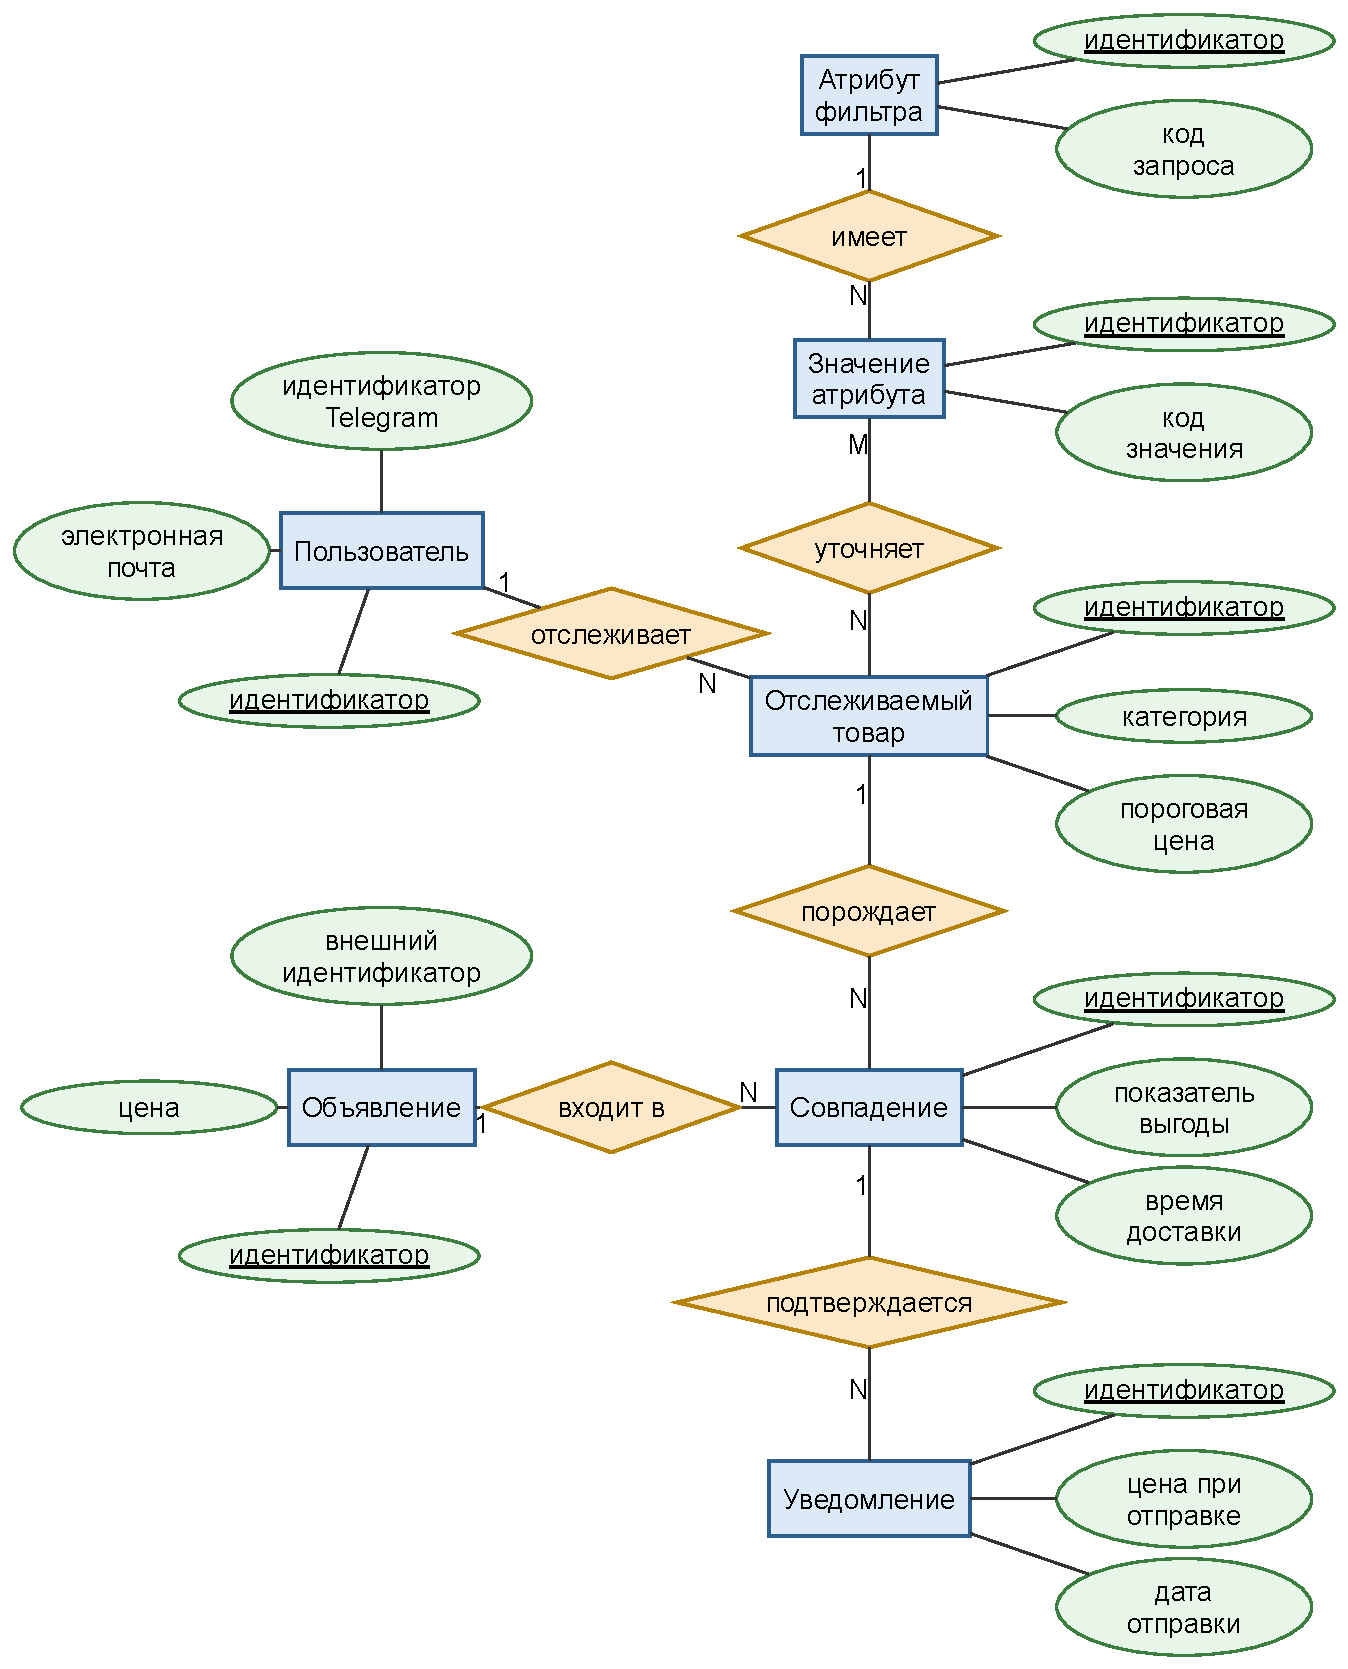
\includegraphics[width=\linewidth]{kufar/er_chen}
	\caption{\textit{ER}-диаграмма базы данных в нотации Питера Чена}
	\label{fig:design:er}
\end{figure}

Сущность «Пользователь»
\begin{itemize}
	\item идентификатор~-- первичный ключ, внутренний номер пользователя в системе;
	\item идентификатор \textit{Telegram}~-- номер учётной записи, по которому бот узнаёт пользователя; должен быть уникальным;
	\item имя учётной записи~-- публичное имя в \textit{Telegram} (может отсутствовать);
	\item имя из профиля~-- имя, которое бот использует в обращениях;
	\item язык интерфейса~-- язык меню и уведомлений (русский или английский);
	\item признак активности~-- снимается, если пользователь заблокировал бота, чтобы система не пыталась отправлять ему сообщения;
	\item признак уведомлений~-- включена ли отправка уведомлений в \textit{Telegram};
	\item электронная почта~-- адрес для копий уведомлений и отчётов (может отсутствовать);
	\item признак подтверждения почты~-- подтверждён ли адрес кодом; без подтверждения письма на адрес не отправляются;
	\item признак почтовых копий~-- отправлять ли копии уведомлений на подтверждённый адрес;
	\item хеш кода подтверждения~-- \textit{HMAC}-свёртка шестизначного кода; сам код в базе данных не хранится;
	\item срок действия кода~-- момент, после которого код подтверждения становится недействительным;
	\item время отправки кода~-- момент последней отправки; ограничивает частоту повторных запросов;
	\item число попыток ввода кода~-- после пятой неудачной попытки код нужно запросить заново;
	\item дата регистрации~-- момент первого обращения пользователя к боту;
	\item дата изменения~-- момент последнего изменения записи.
\end{itemize}

Сущность «Отслеживаемый товар»
\begin{itemize}
	\item идентификатор~-- первичный ключ, уникальный номер товара;
	\item владелец~-- ссылка на пользователя, который добавил товар;
	\item название~-- название товара, по которому ведётся текстовый отбор; в категориях с фильтрами площадки может быть пустым;
	\item категория~-- одна из категорий фиксированного перечня (велосипеды, ноутбуки, аренда квартир, электроника, инструменты и другие);
	\item пороговая цена~-- цена в белорусских рублях, ниже которой объявление считается выгодным;
	\item слова поиска~-- список слов, каждое из которых должно встретиться в заголовке или описании объявления;
	\item слова-исключения~-- список слов, при наличии которых объявление отклоняется;
	\item фильтры площадки~-- набор кодов характеристик и выбранных значений (бренд, размер рамы, число комнат, диапазон площади), которые передаются площадке в поисковом запросе;
	\item признак активности~-- снимается, когда пользователь приостанавливает отслеживание;
	\item дата добавления~-- момент добавления товара; объявления, опубликованные позже этого момента, считаются новыми.
\end{itemize}

Сущность «Объявление»
\begin{itemize}
	\item идентификатор~-- первичный ключ, внутренний номер объявления;
	\item площадка~-- источник объявления; в текущей версии системы это \textit{Kufar.by};
	\item внешний идентификатор~-- номер объявления на площадке; вместе с площадкой однозначно определяет объявление;
	\item заголовок~-- заголовок объявления, заданный продавцом;
	\item описание~-- текст объявления, а при его отсутствии перечень характеристик товара;
	\item цена~-- цена в белорусских рублях (может отсутствовать, если цена договорная);
	\item валюта~-- валюта, в которой указана цена;
	\item ссылка~-- адрес страницы объявления на площадке;
	\item изображения~-- список адресов фотографий товара;
	\item местоположение~-- регион и город или район;
	\item сведения о продавце~-- имя и номер учётной записи продавца на площадке;
	\item состояние~-- состояние товара, указанное продавцом (новое, бывшее в употреблении);
	\item исходный ответ площадки~-- полный ответ по объявлению в формате \textit{JSON};
	\item дата публикации~-- момент размещения объявления на площадке;
	\item первое появление~-- момент, когда система впервые получила объявление;
	\item последнее появление~-- момент последнего получения объявления; по нему удаляются устаревшие записи.
\end{itemize}

Сущность «Совпадение»
\begin{itemize}
	\item идентификатор~-- первичный ключ, уникальный номер совпадения;
	\item отслеживаемый товар~-- ссылка на товар, критериям которого удовлетворило объявление;
	\item объявление~-- ссылка на подошедшее объявление;
	\item показатель выгоды~-- доля, на которую цена объявления ниже пороговой (от нуля до единицы);
	\item подробности отбора~-- тип события (новое объявление или снижение цены), прежняя цена и порог на момент отбора;
	\item время доставки~-- момент успешной отправки уведомления в \textit{Telegram}; пустое значение означает, что совпадение ждёт в очереди;
	\item число попыток~-- количество неудачных отправок; после пятой попытки совпадение исключается из очереди;
	\item текст ошибки~-- причина последней неудачной отправки;
	\item время почтовой копии~-- момент отправки копии уведомления на электронную почту;
	\item число почтовых попыток~-- счётчик неудачных попыток для отдельной почтовой очереди;
	\item оценка пользователя~-- оценка предложения кнопкой под уведомлением («Интересно», «Не то», «Куплю»);
	\item дата создания~-- момент, когда объявление прошло отбор.
\end{itemize}

Сущность «Уведомление»
\begin{itemize}
	\item идентификатор~-- первичный ключ, уникальный номер записи журнала;
	\item получатель~-- ссылка на пользователя, которому отправлено сообщение;
	\item отслеживаемый товар~-- ссылка на товар, по которому пришло уведомление;
	\item объявление~-- ссылка на объявление из уведомления;
	\item совпадение~-- ссылка на совпадение, по которому отправлено сообщение (может отсутствовать);
	\item площадка и внешний идентификатор~-- копия идентификации объявления, по которой проверяется, получал ли пользователь это объявление раньше;
	\item цена при отправке~-- цена объявления на момент отправки; повторно объявление отправляется только по более низкой цене;
	\item показатель выгоды~-- показатель выгоды совпадения на момент отправки;
	\item дата отправки~-- используется для часового и суточного ограничений и для удаления записей старше 90 дней.
\end{itemize}

Сущность «Атрибут фильтра»
\begin{itemize}
	\item идентификатор~-- первичный ключ, уникальный номер характеристики;
	\item категория~-- код категории \textit{Kufar.by}, к которой относится характеристика;
	\item внутреннее имя~-- имя характеристики на площадке; вместе с категорией должно быть уникальным;
	\item код запроса~-- короткий код, под которым площадка принимает характеристику в поисковом запросе;
	\item название~-- название характеристики для меню бота (например, «Производитель»);
	\item частота~-- число объявлений выборки, в которых встретилась характеристика;
	\item дата обновления~-- момент последнего сбора справочника.
\end{itemize}

Сущность «Значение атрибута»
\begin{itemize}
	\item идентификатор~-- первичный ключ, уникальный номер значения;
	\item атрибут~-- ссылка на характеристику, которой принадлежит значение;
	\item код значения~-- код, который передаётся площадке в запросе; вместе с атрибутом должен быть уникальным;
	\item название значения~-- название для кнопки меню (например, «\textit{Trek}»);
	\item родительский регион~-- код региона для значений «город» и «район» (может отсутствовать);
	\item частота~-- число объявлений выборки с этим значением; определяет порядок значений в меню;
	\item дата обновления~-- момент последнего сбора справочника.
\end{itemize}

Связи между сущностями имеют разную мощность. Сущности «Пользователь» и «Отслеживаемый товар» связаны отношением «один ко многим»: один пользователь отслеживает несколько товаров, а каждый товар принадлежит одному пользователю. Между сущностями «Отслеживаемый товар» и «Объявление» существует отношение «многие ко многим»: одно объявление может подойти под товары разных пользователей, а по одному товару находится много объявлений. Это отношение реализовано через сущность «Совпадение», которая связана с товаром и с объявлением отношениями «один ко многим». Для каждой пары товара и объявления хранится одно совпадение: при снижении цены система обновляет его, а не создаёт новое.

Сущности «Совпадение» и «Уведомление» связаны отношением «один ко многим». Если объявление подешевело после первой отправки, пользователь должен получить по тому же совпадению ещё одно уведомление с новой ценой, и в журнале появится вторая запись. В журнале уведомлений получатель хранится напрямую, чтобы часовое и суточное ограничения подсчитывались без обращения к таблицам товаров и совпадений. На концептуальной схеме эта связь не показана: пользователь однозначно определяется через совпадение и отслеживаемый товар.

В справочной части сущности «Атрибут фильтра» и «Значение атрибута» связаны отношением «один ко многим». Сущности «Значение атрибута» и «Отслеживаемый товар» образуют отношение «многие ко многим»: товар уточняется несколькими значениями, а одно значение (например, бренд) выбрано в товарах разных пользователей. В отдельную таблицу эта связь не вынесена. Выбранные коды значений хранятся в самом товаре как набор в формате \textit{JSON}, поскольку в таком же виде они подставляются в поисковый запрос к площадке, а справочник пересобирается каждую неделю и не должен каскадно менять товары пользователей.

Логическая схема базы данных приведена на рисунке~\ref{fig:design:logical}. Каждая сущность стала таблицей с суррогатным первичным ключом \textit{id}, а связи «один ко многим» выражены внешними ключами. Сущности «Пользователь», «Отслеживаемый товар», «Объявление», «Совпадение» и «Уведомление» соответствуют таблицам \textit{users}, \textit{tracked\_products}, \textit{listings}, \textit{matches} и \textit{sent\_notifications}, справочная часть~-- таблицам \textit{kufar\_attributes} и \textit{kufar\_attribute\_values}. Кроме таблиц, соответствующих сущностям модели, в схему входит резервная таблица пользовательских атрибутов товара \textit{custom\_attributes}. Она создана для будущего расширения системы, в текущей версии не заполняется и в концептуальную модель не включена.

\begin{figure}[H]
	\centering
	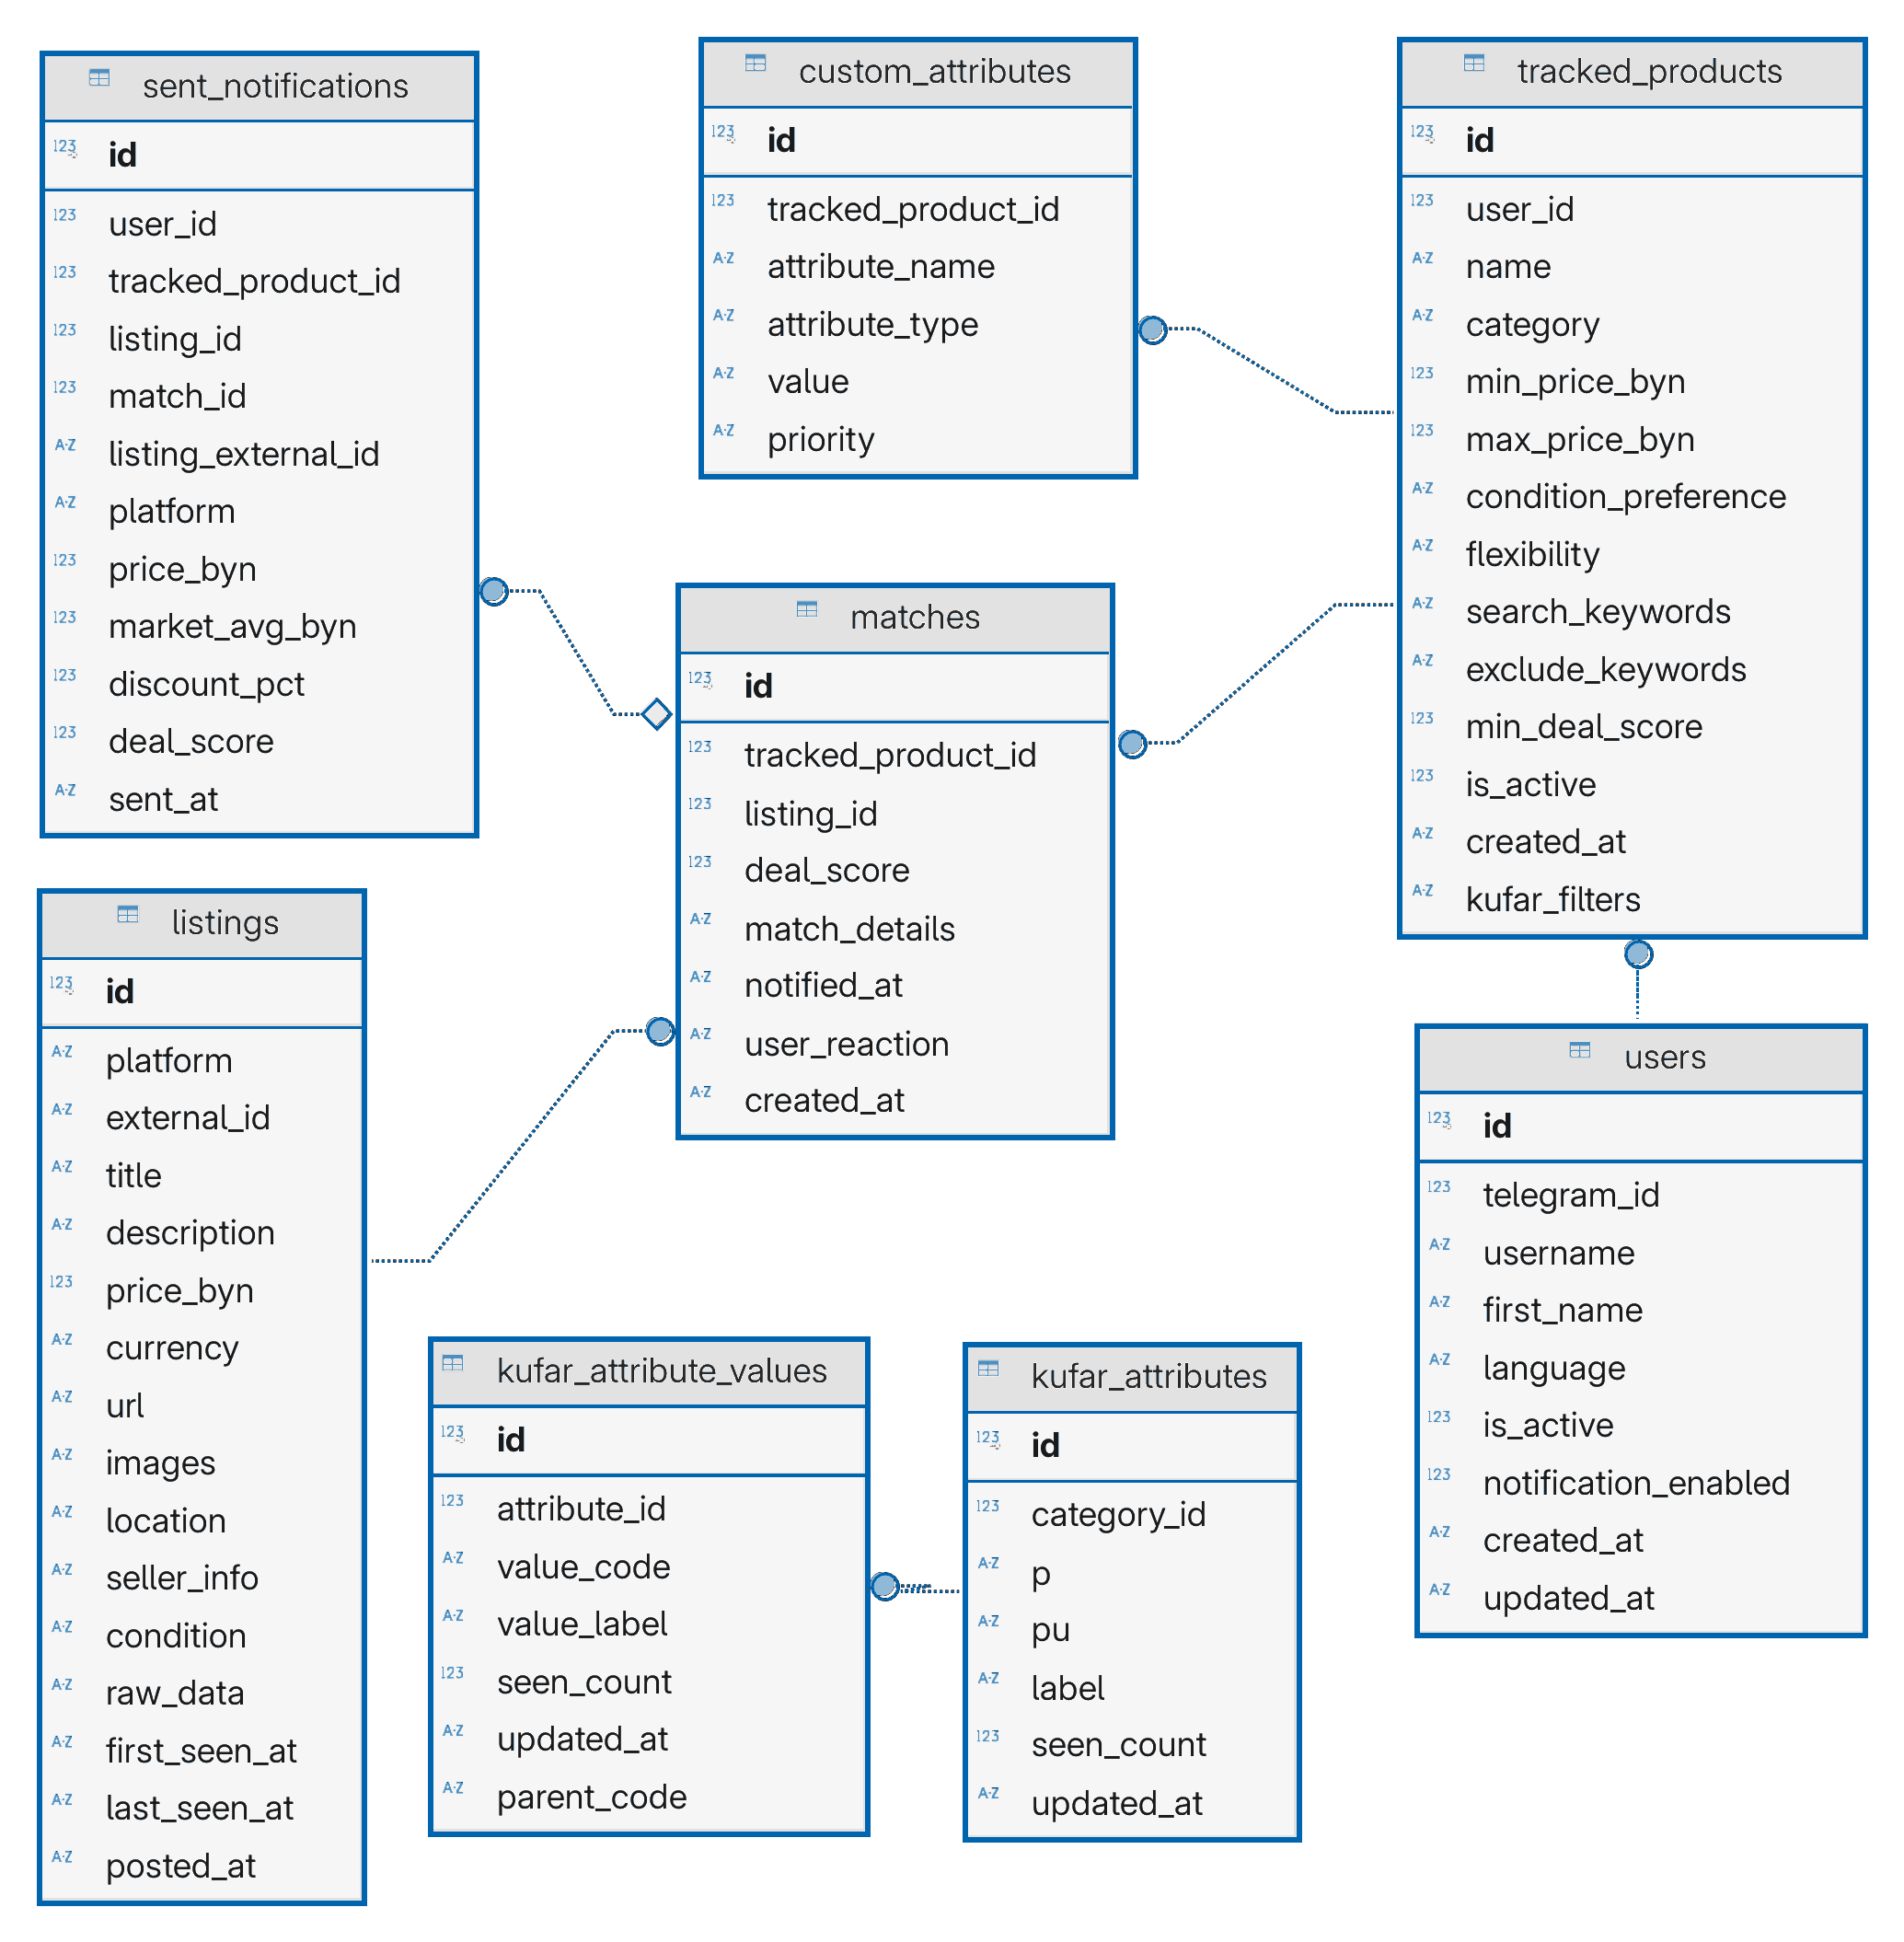
\includegraphics[width=\linewidth]{kufar/physical}
	\caption{Логическая схема базы данных}
	\label{fig:design:logical}
\end{figure}

Разделение данных на пользовательские, рабочие и справочные определяет дальнейшую работу со схемой. Пользовательские таблицы меняются только по командам пользователя и невелики. Рабочие таблицы растут с каждым циклом опроса, поэтому для них предусмотрено удаление устаревших записей и индексы под запросы цикла. Справочные таблицы перезаписываются по расписанию и на пользовательские данные не ссылаются.


\subsection{Проектирование системы}
\label{sec:design:system}

До начала реализации нужно определить границы системы: какие действия выполняет пользователь, что система делает сама по расписанию и с какими внешними сервисами обменивается данными. Эти границы описаны диаграммами вариантов использования и контекста. Поведение системы во время работы показано диаграммой последовательности и схемой алгоритма мониторинга. Диаграммы строились как рабочий материал для реализации: по ним определялось, какие данные читает и записывает каждая часть системы и в каком порядке.

\subsubsection{Диаграмма вариантов использования}

Диаграмма вариантов использования (\textit{Use Case Diagram}) описывает функциональные требования к системе с точки зрения тех, кто с ней взаимодействует. На ней показано, что система делает для пользователя, без деталей реализации. Диаграмма приведена на рисунке~\ref{fig:design:usecase}.

\begin{figure}[H]
	\centering
	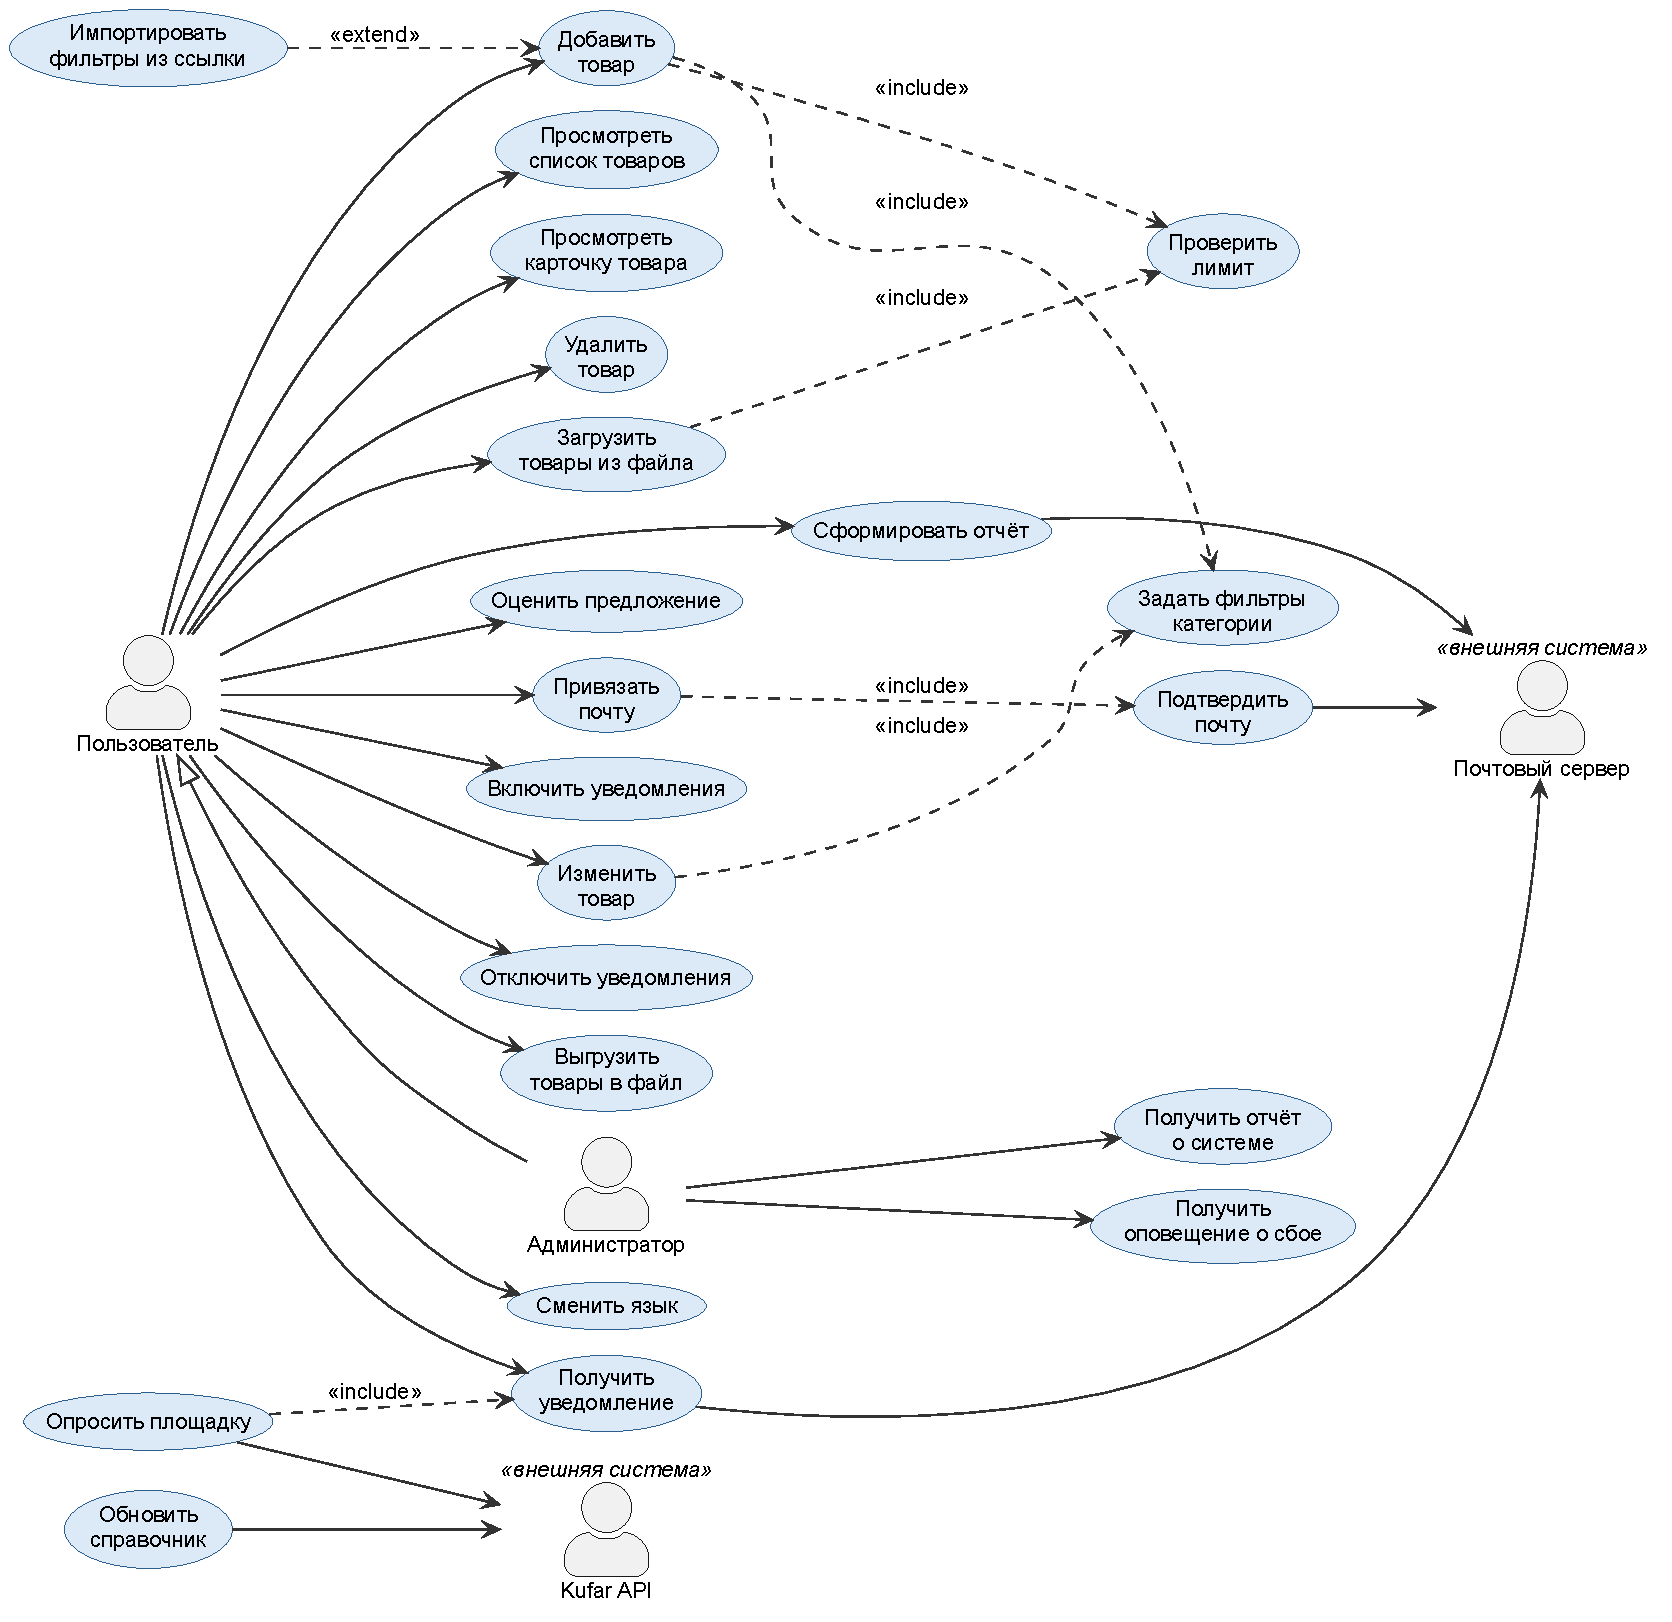
\includegraphics[width=0.95\linewidth]{kufar/usecase}
	\caption{Диаграмма вариантов использования}
	\label{fig:design:usecase}
\end{figure}

На диаграмме выделены следующие действующие лица:
\begin{itemize}
	\item «Пользователь»~-- человек, который работает с ботом в \textit{Telegram}: добавляет, просматривает, изменяет и удаляет отслеживаемые товары, получает уведомления о выгодных предложениях и оценивает их, выгружает и загружает список товаров файлом, формирует отчёты, меняет язык интерфейса и привязывает электронную почту;
	\item «Администратор»~-- пользователь, идентификатор которого указан в конфигурации системы; наследует все возможности «Пользователя», получает повышенный лимит отслеживаемых товаров, отчёт о состоянии системы и служебные оповещения о сбоях;
	\item «\textit{Kufar API}»~-- внешняя система, поисковый интерфейс площадки. Из него система получает объявления при мониторинге и образцы объявлений при обновлении справочника фильтров;
	\item «Почтовый сервер»~-- внешняя система, через которую отправляются коды подтверждения, копии уведомлений и отчёты.
\end{itemize}

Названия вариантов использования заданы глаголами, поскольку вариант описывает действие, а не объект. Операции над отслеживаемым товаром образуют полный набор: «Добавить товар», «Просмотреть список товаров», «Просмотреть карточку товара», «Изменить товар» и «Удалить товар». Такой набор из пяти операций принято обозначать сокращением \textit{CRUDL} по первым буквам английских названий создания, чтения, изменения, удаления и получения списка.

Варианты «Опросить площадку» и «Обновить справочник» запускаются не человеком, а планировщиком системы по расписанию. Добавление товара включает выбор фильтров категории и проверку лимита, изменение товара включает тот же выбор фильтров, а импорт фильтров из ссылки \textit{Kufar.by} расширяет добавление как альтернативный способ задать критерии. Привязка электронной почты включает её подтверждение кодом, без которого письма на адрес не отправляются.

Модель вариантов использования разграничивает функции системы между двумя ролями. Пользователю доступна вся работа с отслеживаемыми товарами, уведомлениями, отчётами и почтой. Администратор получает эти же функции и, кроме них, средства контроля: отчёт о состоянии системы и оповещения о сбоях. Большинство вариантов использования заканчивается записью в базу данных, а получение уведомлений целиком построено на данных, накопленных предыдущими циклами опроса.

\subsubsection{Диаграмма контекста}

Диаграмма контекста первого уровня модели \textit{C4} показывает систему как единое целое вместе с людьми и внешними системами, с которыми происходит обмен данными. Внутреннее устройство на этом уровне не раскрывается [5]. Диаграмма приведена на рисунке~\ref{fig:design:context}.

\begin{figure}[H]
	\centering
	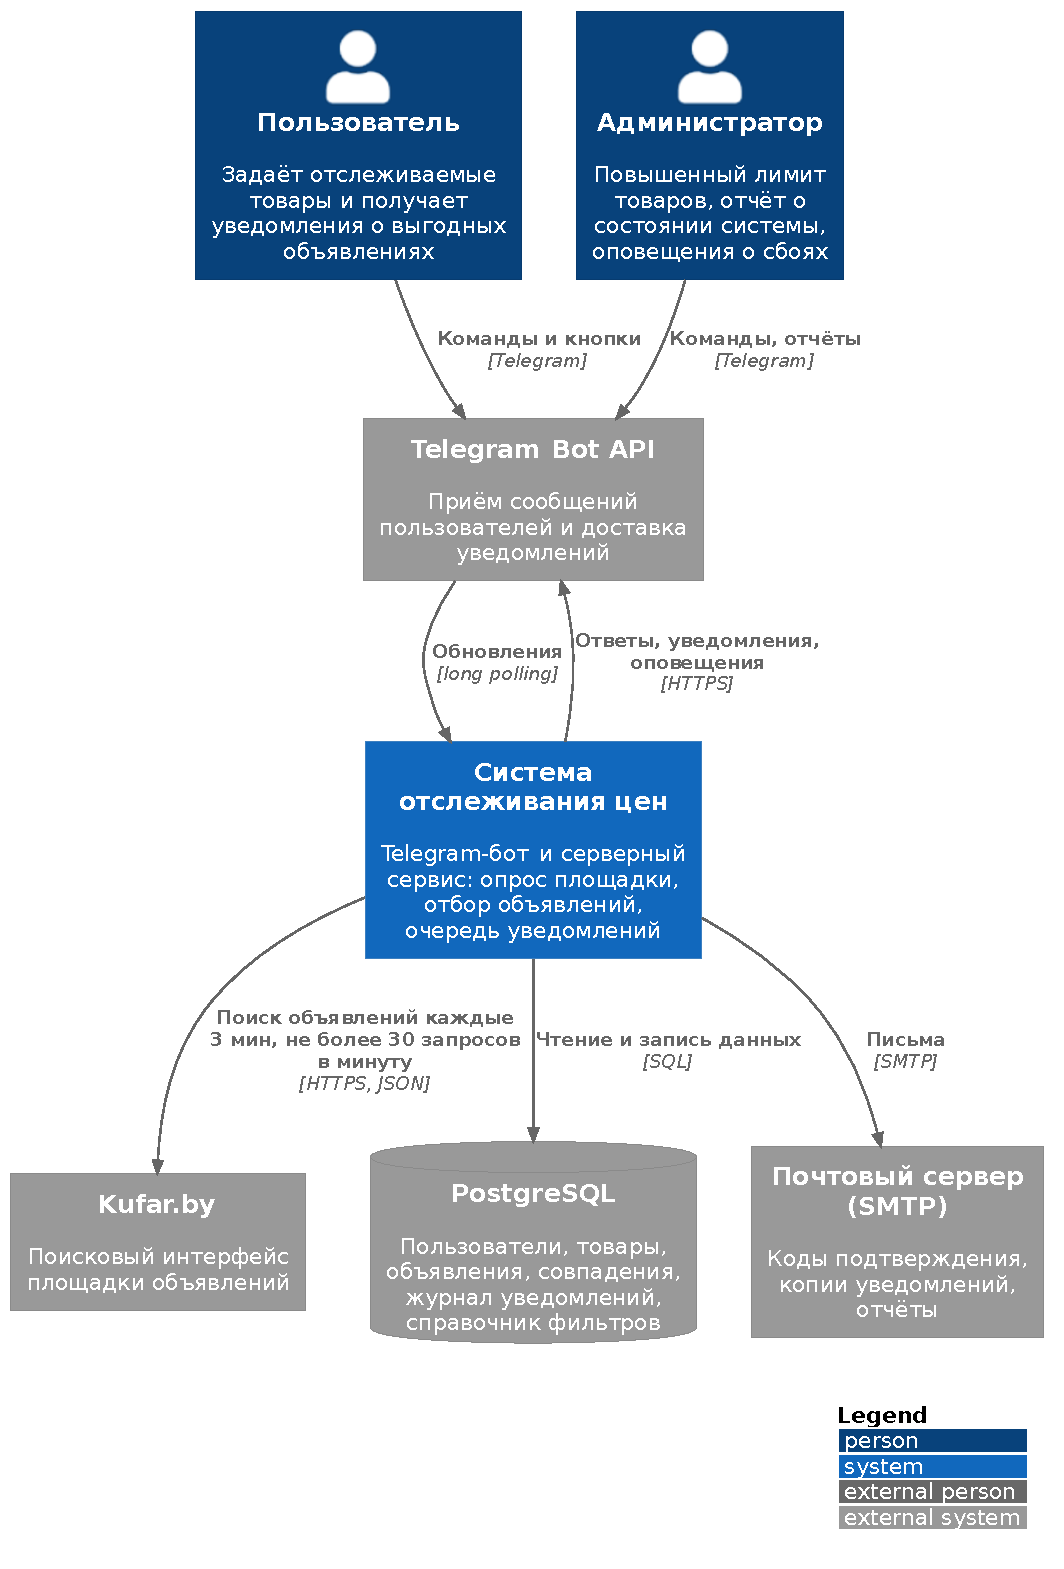
\includegraphics[width=0.6\linewidth]{kufar/context}
	\caption{Диаграмма контекста системы (\textit{C4}, уровень 1)}
	\label{fig:design:context}
\end{figure}

В центре диаграммы находится система отслеживания цен. Пользователь и администратор обращаются к ней не напрямую, а через \textit{Telegram}: команды и нажатия кнопок попадают в \textit{Telegram Bot API}, откуда система забирает их методом длинного опроса (\textit{long polling}). Тем же каналом система отправляет ответы, уведомления и служебные оповещения [6].

Площадка \textit{Kufar.by} выступает источником данных. Система обращается к её поисковому интерфейсу по \textit{HTTPS} и получает объявления в формате \textit{JSON}. Обращения ограничены: опрос выполняется раз в 3 минуты, и за минуту отправляется не более 30 запросов.

Все данные системы хранит СУБД \textit{PostgreSQL}. Система обращается к ней SQL-запросами. Почтовый сервер получает от системы письма с кодами подтверждения, копиями уведомлений и отчётами по протоколу \textit{SMTP}.

Граница системы проходит так, что ни одна внешняя система не обращается к ней сама по себе. Система опрашивает \textit{Telegram} и площадку по своей инициативе и в своём темпе. Это упрощает защиту: снаружи доступен только программный интерфейс для бота, закрытый секретным ключом.

\subsubsection{Диаграмма последовательности}

Диаграмма последовательности (\textit{Sequence Diagram}) показывает порядок обмена сообщениями между участниками во времени. Работа системы разделена на две независимые части, которые запускает планировщик: цикл опроса площадки и доставку уведомлений. Каждая часть показана отдельной диаграммой на рисунках~\ref{fig:design:sequence:scrape} и~\ref{fig:design:sequence:deliver}.

\begin{figure}[H]
	\centering
	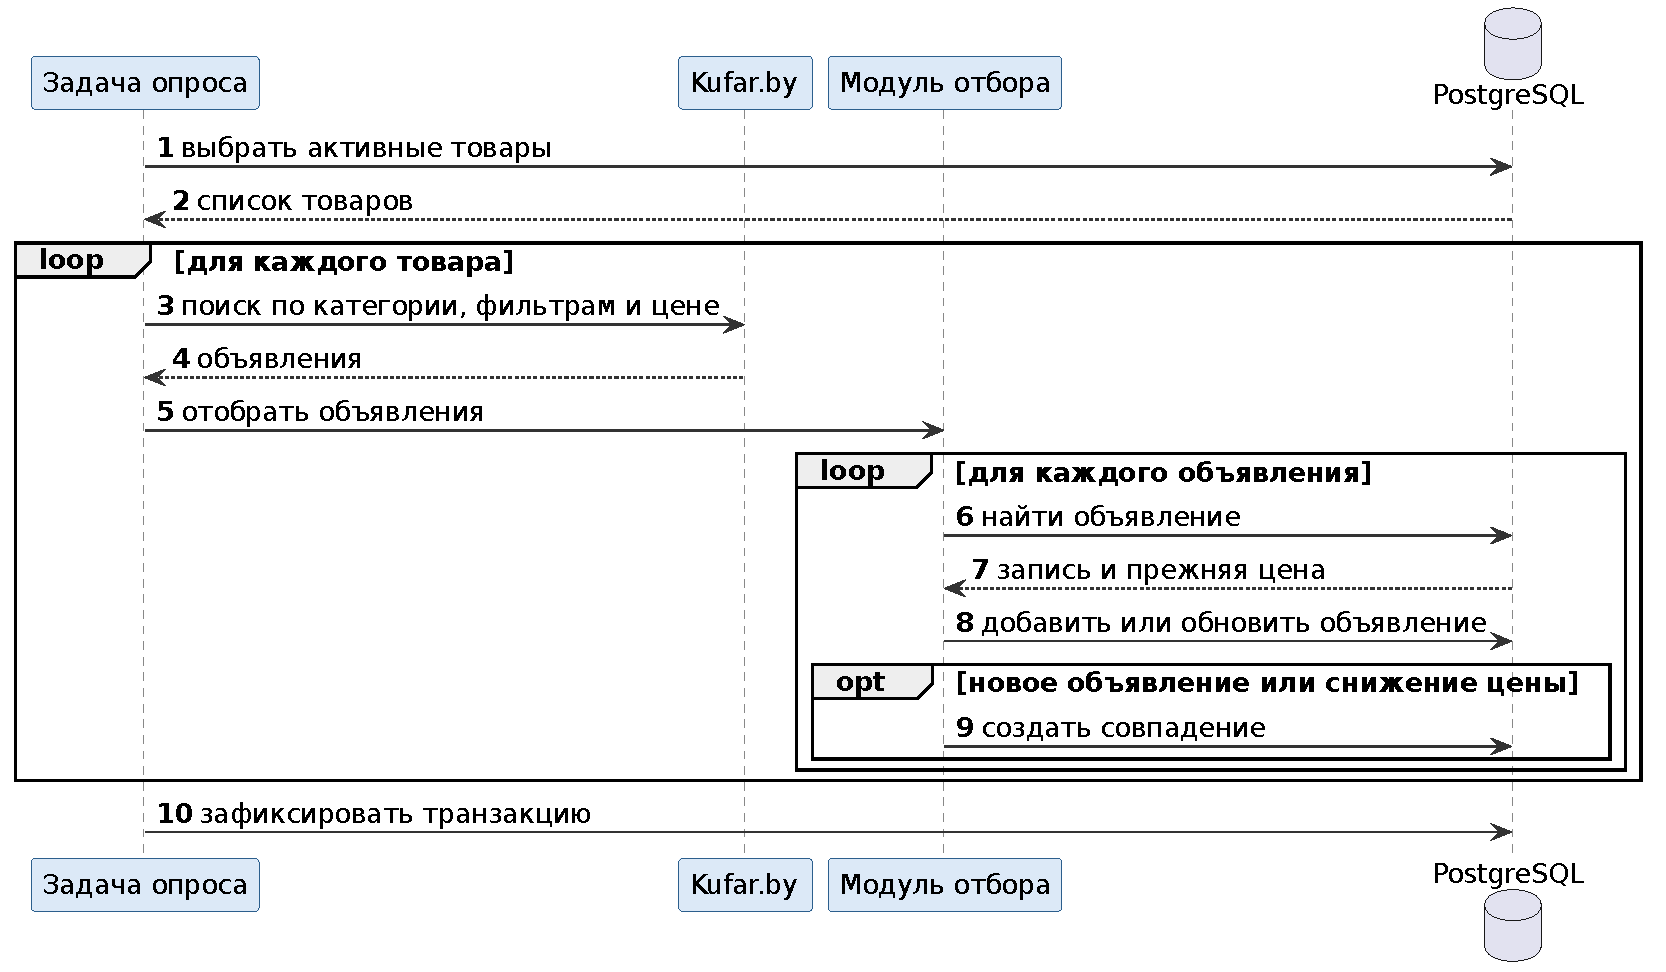
\includegraphics[width=\linewidth]{kufar/sequence_scrape}
	\caption{Диаграмма последовательности цикла опроса площадки}
	\label{fig:design:sequence:scrape}
\end{figure}

Цикл опроса выполняется каждые 3 минуты. Задача опроса выбирает из базы данных активные отслеживаемые товары и для каждого отправляет площадке поисковый запрос с категорией, фильтрами и ограничением цены сверху, равным порогу товара. При отказе площадки с кодом 403 или 429 цикл прерывается сразу, не дожидаясь ответа по остальным товарам, и задача увеличивает паузу до следующего опроса.

При успешном ответе объявления передаются модулю отбора. Для каждого объявления модуль ищет в базе данных запись по паре «площадка~-- внешний идентификатор». Если записи нет, объявление добавляется, если есть, обновляется, и модуль получает прежнюю цену. Затем объявление проверяется по цене, словам-исключениям и названию. Совпадение создаётся, только если объявление опубликовано после добавления товара или его цена снизилась. Изменения всего цикла фиксируются одной транзакцией.

\begin{figure}[H]
	\centering
	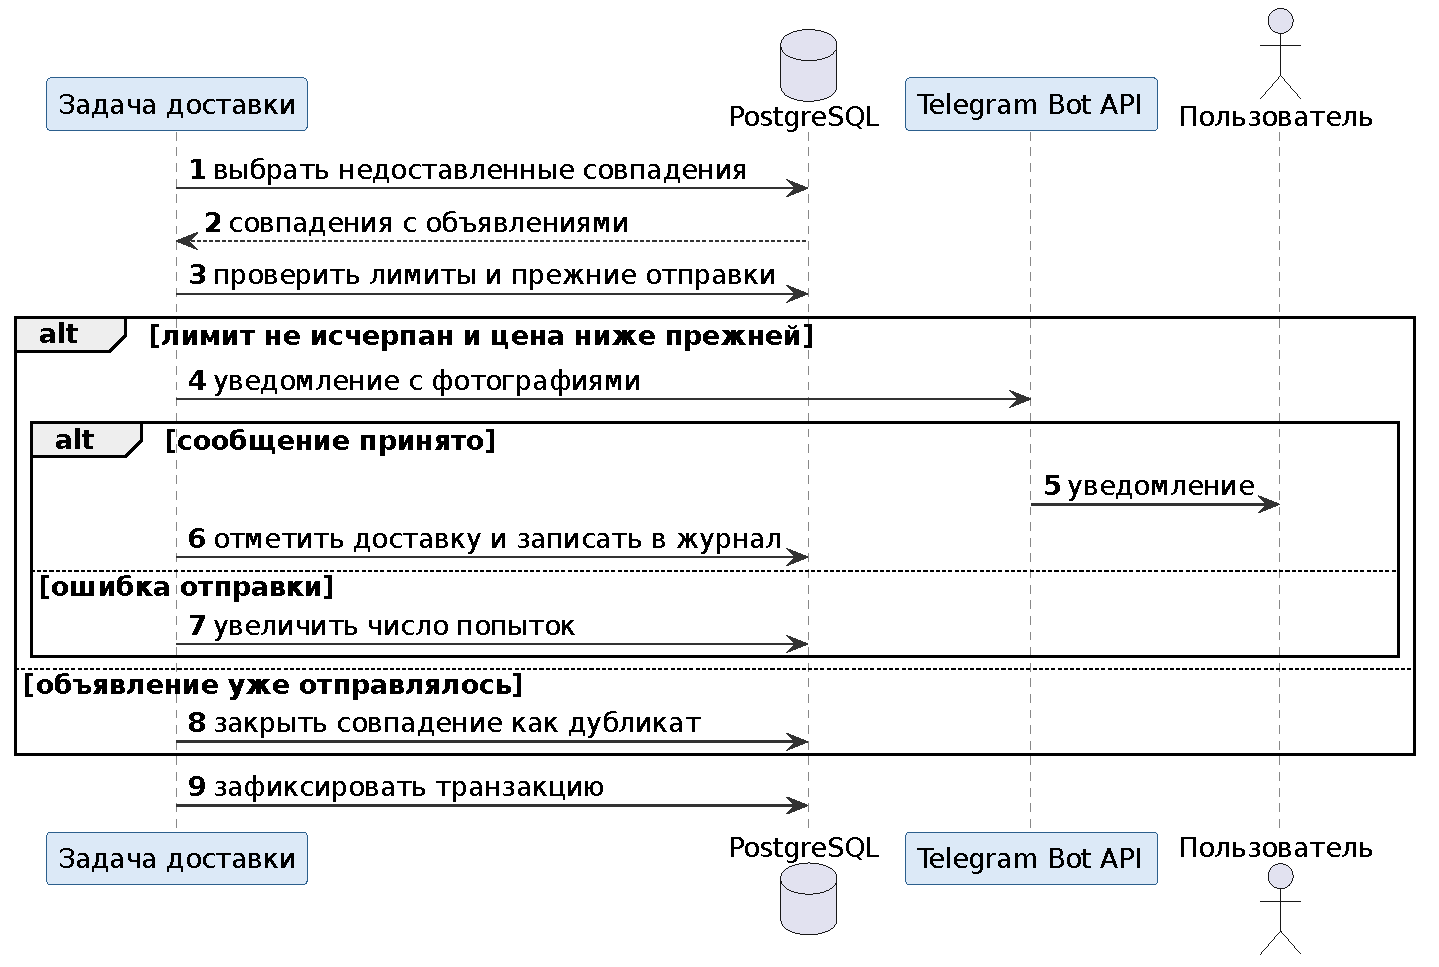
\includegraphics[width=\linewidth]{kufar/sequence_deliver}
	\caption{Диаграмма последовательности доставки уведомлений}
	\label{fig:design:sequence:deliver}
\end{figure}

Доставка выполняется каждую минуту отдельной задачей. Задача выбирает недоставленные совпадения, у которых меньше пяти неудачных попыток и возраст не больше трёх суток, проверяет часовой и суточный лимиты и цену прежних отправок этого объявления. Если объявление уже приходило пользователю по такой же или меньшей цене, совпадение закрывается как дубликат. Иначе сообщение уходит через \textit{Telegram Bot API}. При успехе совпадение отмечается доставленным и в журнал уведомлений добавляется запись, при ошибке увеличивается счётчик попыток и сохраняется текст ошибки.

Опрос и доставка разделены намеренно. Медленный ответ \textit{Telegram} не задерживает опрос площадки, а совпадение, которое не удалось отправить, остаётся в базе данных и не теряется вместе с циклом. Очередью уведомлений в этой схеме служит обычная таблица совпадений, в которой недоставленные записи отличаются пустым временем доставки.

\subsubsection{Схемы алгоритмов мониторинга и доставки уведомлений}

Схемы алгоритмов детализируют логику, которая на диаграммах последовательности показана сообщениями. Схемы выполнены по ГОСТ~19.701–90: действие обозначено прямоугольником, условие~-- ромбом, начало и конец~-- прямоугольником со скруглёнными углами, ввод и вывод данных~-- параллелограммом. Символ «Начало» стоит вверху по центру, символ «Конец» на каждой схеме один и стоит внизу по центру. Линии потока проведены только по горизонтали и вертикали; стрелка поставлена там, где поток идёт не сверху вниз и не слева направо, то есть на возвратах к началу цикла и на боковых ветвях. Схема алгоритма цикла опроса приведена на рисунке~\ref{fig:design:algorithm:scrape}.

\begin{figure}[H]
	\centering
	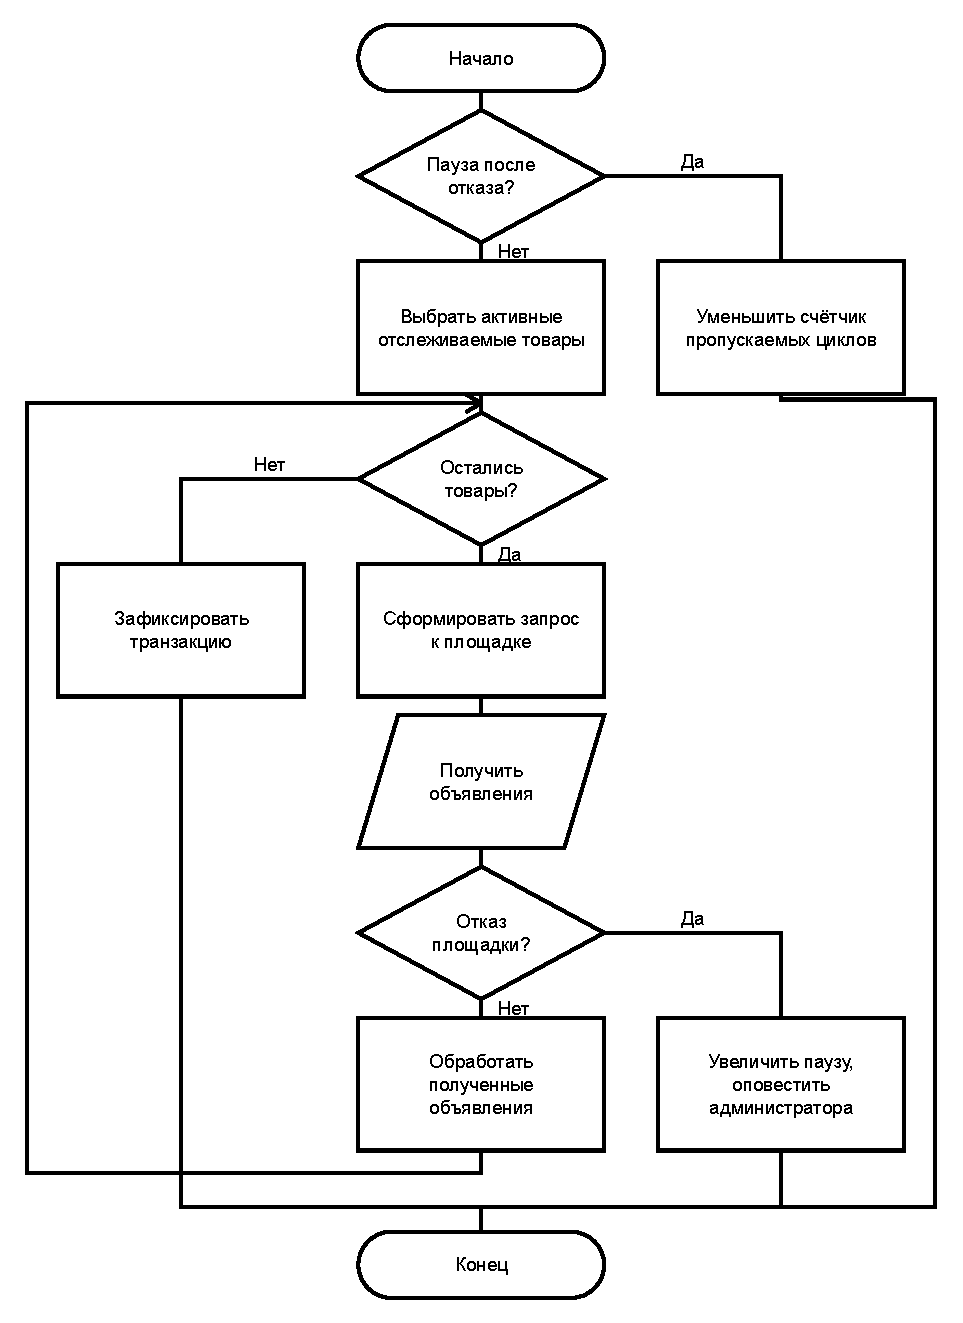
\includegraphics{kufar/algorithm_scrape}
	\caption{Схема алгоритма цикла опроса площадки}
	\label{fig:design:algorithm:scrape}
\end{figure}

Алгоритм начинается с проверки паузы. Если на одном из предыдущих циклов площадка отказала в обслуживании, текущий цикл пропускается и счётчик пропускаемых циклов уменьшается на единицу. Пауза растёт при каждом отказе подряд: 1, 2, 4, 8 и не более 16 циклов. Первый успешный цикл после блокировки сбрасывает её. При интервале в 3 минуты самая длинная пауза составляет 48 минут.

Затем выбираются активные отслеживаемые товары, и для каждого формируется запрос к площадке. Товары обрабатываются строго по очереди, и нагрузка на площадку остаётся в пределах 30 запросов в минуту. Отказ площадки на любом товаре завершает весь цикл с оповещением администратора. Продолжать запросы в прежнем темпе после отказа означало бы превратить временное ограничение в длительную блокировку.

Обработка каждого полученного объявления вынесена в отдельную схему на рисунке~\ref{fig:design:algorithm:listing}. Объявление сначала сохраняется в базе данных, даже если потом будет отклонено: сохранённая цена нужна следующим циклам, потому что только сравнение с ней показывает снижение цены. Проверка релевантности состоит из трёх условий: цена ниже порога, в тексте нет слов-исключений, в заголовке или описании есть все слова названия товара. Прошедшее проверку объявление становится совпадением, только если оно опубликовано после добавления товара или подешевело. Объявления, которые были на площадке до добавления товара и с тех пор не подешевели, пользователь мог просмотреть сам при настройке поиска, а самые дешёвые из них получил при мгновенном поиске, поэтому о них система не сообщает.

\begin{figure}[H]
	\centering
	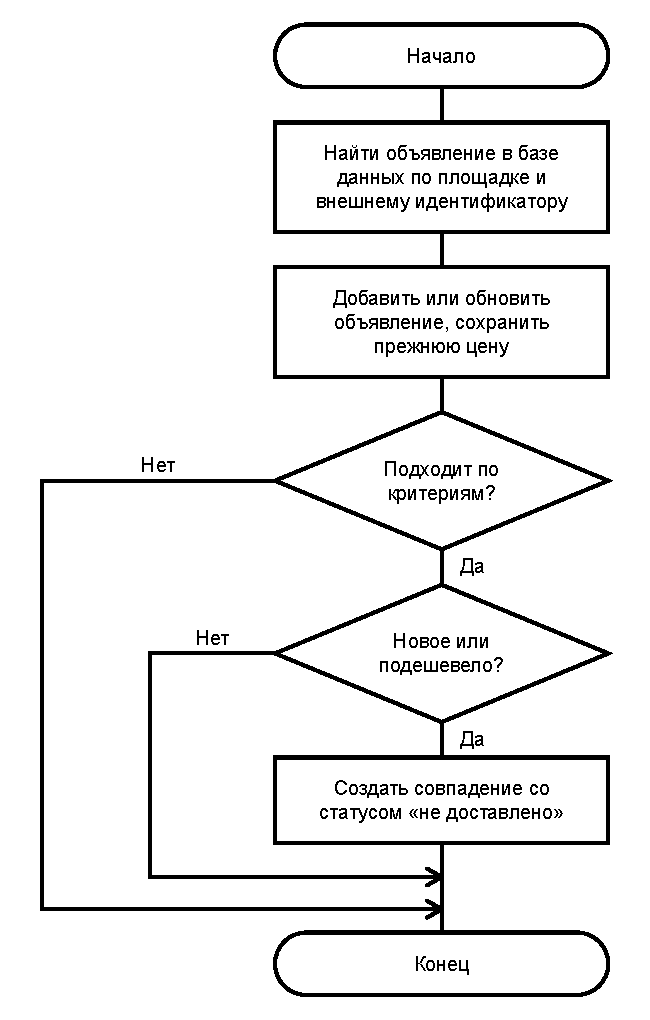
\includegraphics{kufar/algorithm_listing}
	\caption{Схема алгоритма обработки полученного объявления}
	\label{fig:design:algorithm:listing}
\end{figure}

Очередь доставки обрабатывает схема на рисунке~\ref{fig:design:algorithm:deliver}. Для каждого совпадения проверяются три условия по порядку: не исчерпан ли лимит уведомлений, не отправлялось ли объявление по такой же или меньшей цене и принял ли \textit{Telegram} сообщение. Первое условие оставляет совпадение в очереди до следующего часа или дня, второе закрывает его как дубликат, третье определяет, будет ли совпадение отмечено доставленным или получит ещё одну попытку. Изменения каждого запуска доставки фиксируются транзакцией, поэтому отметка о доставке и запись в журнале уведомлений сохраняются вместе.

\begin{figure}[H]
	\centering
	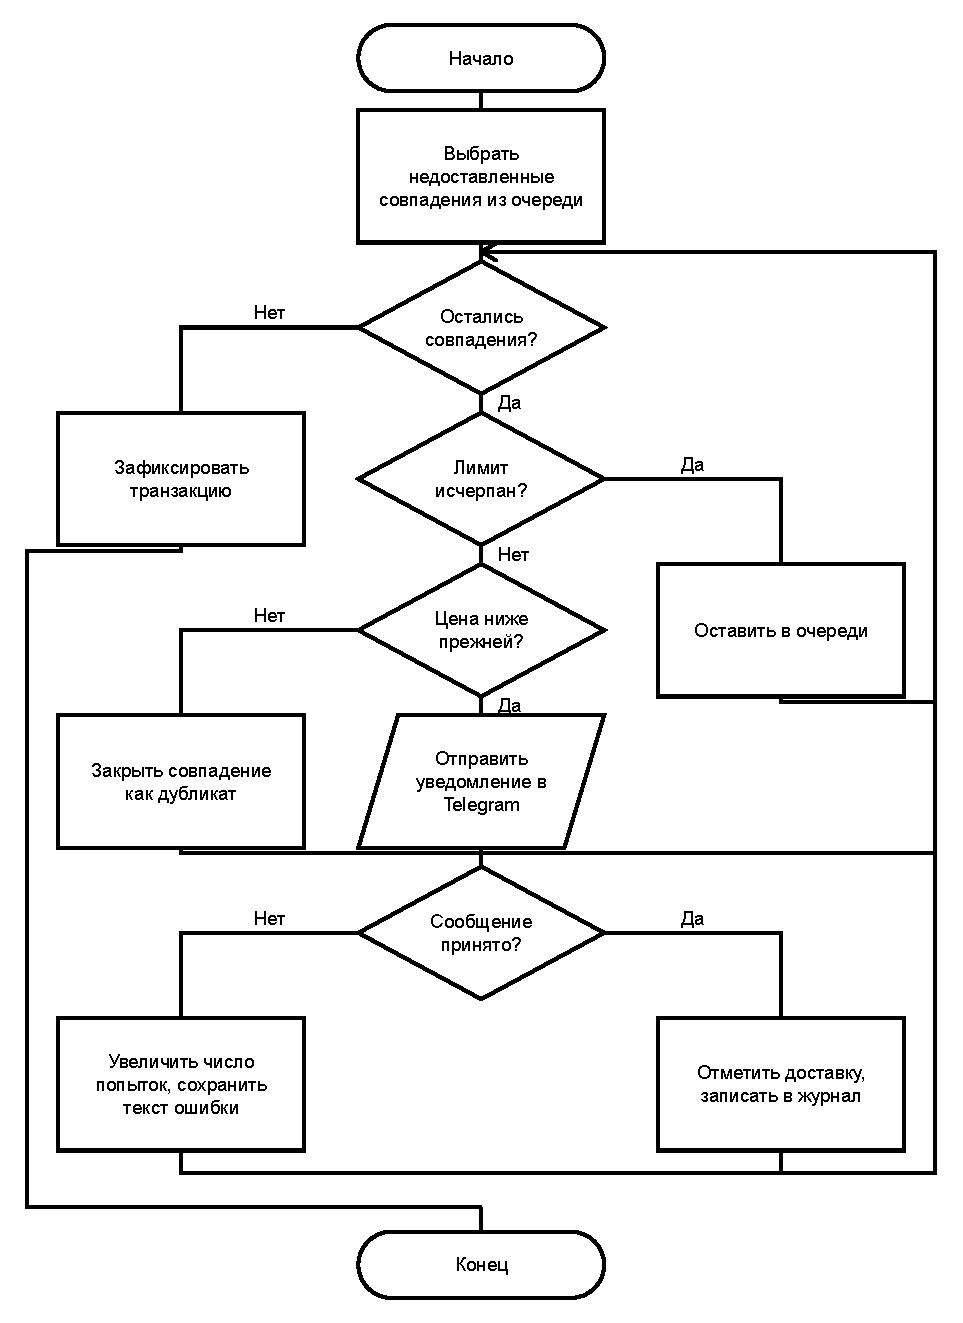
\includegraphics{kufar/algorithm_deliver}
	\caption{Схема алгоритма доставки уведомлений}
	\label{fig:design:algorithm:deliver}
\end{figure}



	\section{Разработка системы}
\label{sec:development}

\subsection{Выбор средств реализации}
\label{sec:development:tools}

Средства реализации выбирались под три особенности задачи. Данные изменяются одновременно несколькими процессами. Большую часть времени система ждёт ответов от внешних сервисов: площадки, \textit{Telegram}, почтового сервера. Система работает круглосуточно на одном сервере и должна переживать перезапуски без потери данных.

\subsubsection{Язык программирования}

Система написана на \textit{Python}~3.11. В языке есть встроенная поддержка асинхронного выполнения, при котором один процесс обслуживает множество одновременных операций ввода-вывода, не создавая поток на каждую из них. Пока система ждёт ответа площадки на один запрос, параллельно обрабатываются команды пользователей и отправляются уведомления. Для \textit{Python} существуют зрелые асинхронные библиотеки для всех внешних сервисов системы: \textit{Telegram}, \textit{HTTP}, \textit{PostgreSQL}.

\subsubsection{Выбор СУБД}

В качестве СУБД выбрана \textit{PostgreSQL}~16. Наряду с ней рассматривались \textit{MySQL}, встраиваемая \textit{SQLite} и документоориентированная \textit{MongoDB}. Сравнение по свойствам, значимым для задачи, приведено в таблице~\ref{table:development:dbms} [7].

\begin{table}[ht]
\caption{Сравнение СУБД по требованиям системы}
\label{table:development:dbms}
\centering
	\begin{tabular}{|>{\raggedright}m{0.32\textwidth}
	                |>{\centering}m{0.13\textwidth}
	                |>{\centering}m{0.13\textwidth}
	                |>{\centering}m{0.13\textwidth}
	                |>{\centering\arraybackslash}m{0.13\textwidth}|}
	\hline
	\centering Свойство & \textit{Post\-greSQL} & \textit{MySQL} & \textit{SQLite} & \textit{Mongo\-DB} \\
	\hline Работа как отдельный сетевой сервер & $+$ & $+$ & $-$ & $+$ \\
	\hline Одновременная запись несколькими процессами & $+$ & $+$ & $-$ & $+$ \\
	\hline Внешние ключи & $+$ & $+$ & $+$ & $-$ \\
	\hline Откат изменений схемы в транзакции & $+$ & $-$ & $+$ & не требуется \\
	\hline Хранение \textit{JSON}-документов & $+$ & $+$ & частично & $+$ \\
	\hline Рекомендательные блокировки & $+$ & $+$ & $-$ & $-$ \\
	\hline
	\end{tabular}
\end{table}

\textit{SQLite} хранит базу в одном файле и в каждый момент допускает только одну пишущую транзакцию. Первая версия бота работала на ней в одном процессе. Когда система была разделена на несколько сервисов, работающих с общими данными, от встраиваемой базы пришлось отказаться в пользу сетевой СУБД. \textit{MongoDB} не поддерживает внешние ключи, а связи между пользователем, товаром, совпадением и уведомлением составляют основу модели данных, и их целостность пришлось бы контролировать вручную. \textit{MySQL} подошла бы по большинству свойств, однако изменение схемы в ней не откатывается вместе с транзакцией: миграция, прерванная на середине, оставляет базу в промежуточном состоянии.

\textit{PostgreSQL} закрывает все требования. Внешние ключи и транзакции обеспечивают целостность цепочки от пользователя до уведомления. Тип \textit{JSON} хранит данные переменной структуры: фильтры площадки, у которых набор характеристик свой для каждой категории, списки слов, адреса фотографий, исходный ответ площадки. Выделять под них отдельные таблицы не нужно. Рекомендательная блокировка (\textit{advisory lock}) защищает от одновременного применения миграций несколькими экземплярами сервиса при запуске.

\subsubsection{Доступ к базе данных и миграции}

Запросы к базе данных записываются на SQL и выполняются через асинхронный драйвер \textit{asyncpg}, который работает с сетевым протоколом \textit{PostgreSQL} напрямую. Структура базы данных описывается версионированными миграциями под управлением \textit{Alembic}. Каждая миграция описывается SQL-скриптом перехода между двумя версиями схемы и содержит обратный переход. Миграции применяются автоматически при запуске серверного сервиса, поэтому схема рабочей базы всегда соответствует версии кода [8, 9].

\subsubsection{Серверный интерфейс}

Программный интерфейс, через который бот получает и изменяет данные, построен на веб-фреймворке \textit{FastAPI} и запускается сервером \textit{uvicorn}. \textit{FastAPI} асинхронный и проверяет входные данные по объявленным схемам \textit{pydantic}: запрос с отрицательной ценой или слишком длинным названием отклоняется до обращения к базе данных. Описание интерфейса формируется автоматически по коду. \textit{Flask} требует для тех же возможностей набора расширений, а \textit{Django} рассчитан на веб-приложения с шаблонами страниц и административной панелью, которые системе не нужны [10].

\subsubsection{Работа с \textit{Telegram}}

Бот построен на библиотеке \textit{aiogram}~3. Библиотека асинхронная и поддерживает конечные автоматы для многошаговых диалогов: добавление товара проходит до восьми шагов, и на каждом шаге сохраняется состояние диалога пользователя. Обработчики разделяются по маршрутизаторам, а общая логика, например определение пользователя по каждому входящему сообщению, выносится в промежуточный слой [11].

\subsubsection{Периодические задачи}

Опрос площадки, доставка уведомлений, рассылка почтовых копий, очистка устаревших данных и обновление справочника фильтров запускаются планировщиком \textit{APScheduler} внутри серверного сервиса. Отдельный брокер сообщений, как у \textit{Celery}, для пяти задач на одном сервере не требуется, а системный \textit{cron} не даёт запретить повторный запуск задачи, пока предыдущий ещё не завершился [12].

\subsubsection{Вспомогательные библиотеки}

Запросы к площадке выполняет асинхронный клиент \textit{aiohttp}, бот обращается к серверному интерфейсу через \textit{httpx}. Нечёткое сравнение строк при проверке названия товара выполняет \textit{rapidfuzz}. Отчёты в формате \textit{Excel} формирует \textit{openpyxl}. Журнал работы с ротацией файлов ведёт \textit{loguru}. Тесты написаны на \textit{pytest}.

\subsubsection{Развёртывание}

Все компоненты запускаются в контейнерах \textit{Docker} и описаны одним файлом \textit{Docker Compose}: СУБД, серверный сервис, бот, резервное копирование, служба мониторинга контейнеров и почтовый сервер для проверки писем. Такой способ воспроизводит окружение на любом сервере одной командой, автоматически перезапускает упавшие контейнеры и хранит данные базы в отдельном томе, который не пропадает при пересборке [13].


\subsection{Реализация базы данных}
\label{sec:development:database}

\subsubsection{Физическая схема}

Физическая схема получена из логической (рисунок~\ref{fig:design:logical}) по обычным правилам: каждая сущность стала таблицей, каждый атрибут~-- столбцом, связи «один ко многим» выражены внешними ключами в таблице на стороне «многие». Физическая схема базы данных приведена на рисунке~\ref{fig:development:physical}, назначение таблиц и характер их роста~-- в таблице~\ref{table:development:tables}.

\begin{figure}[H]
	\centering
	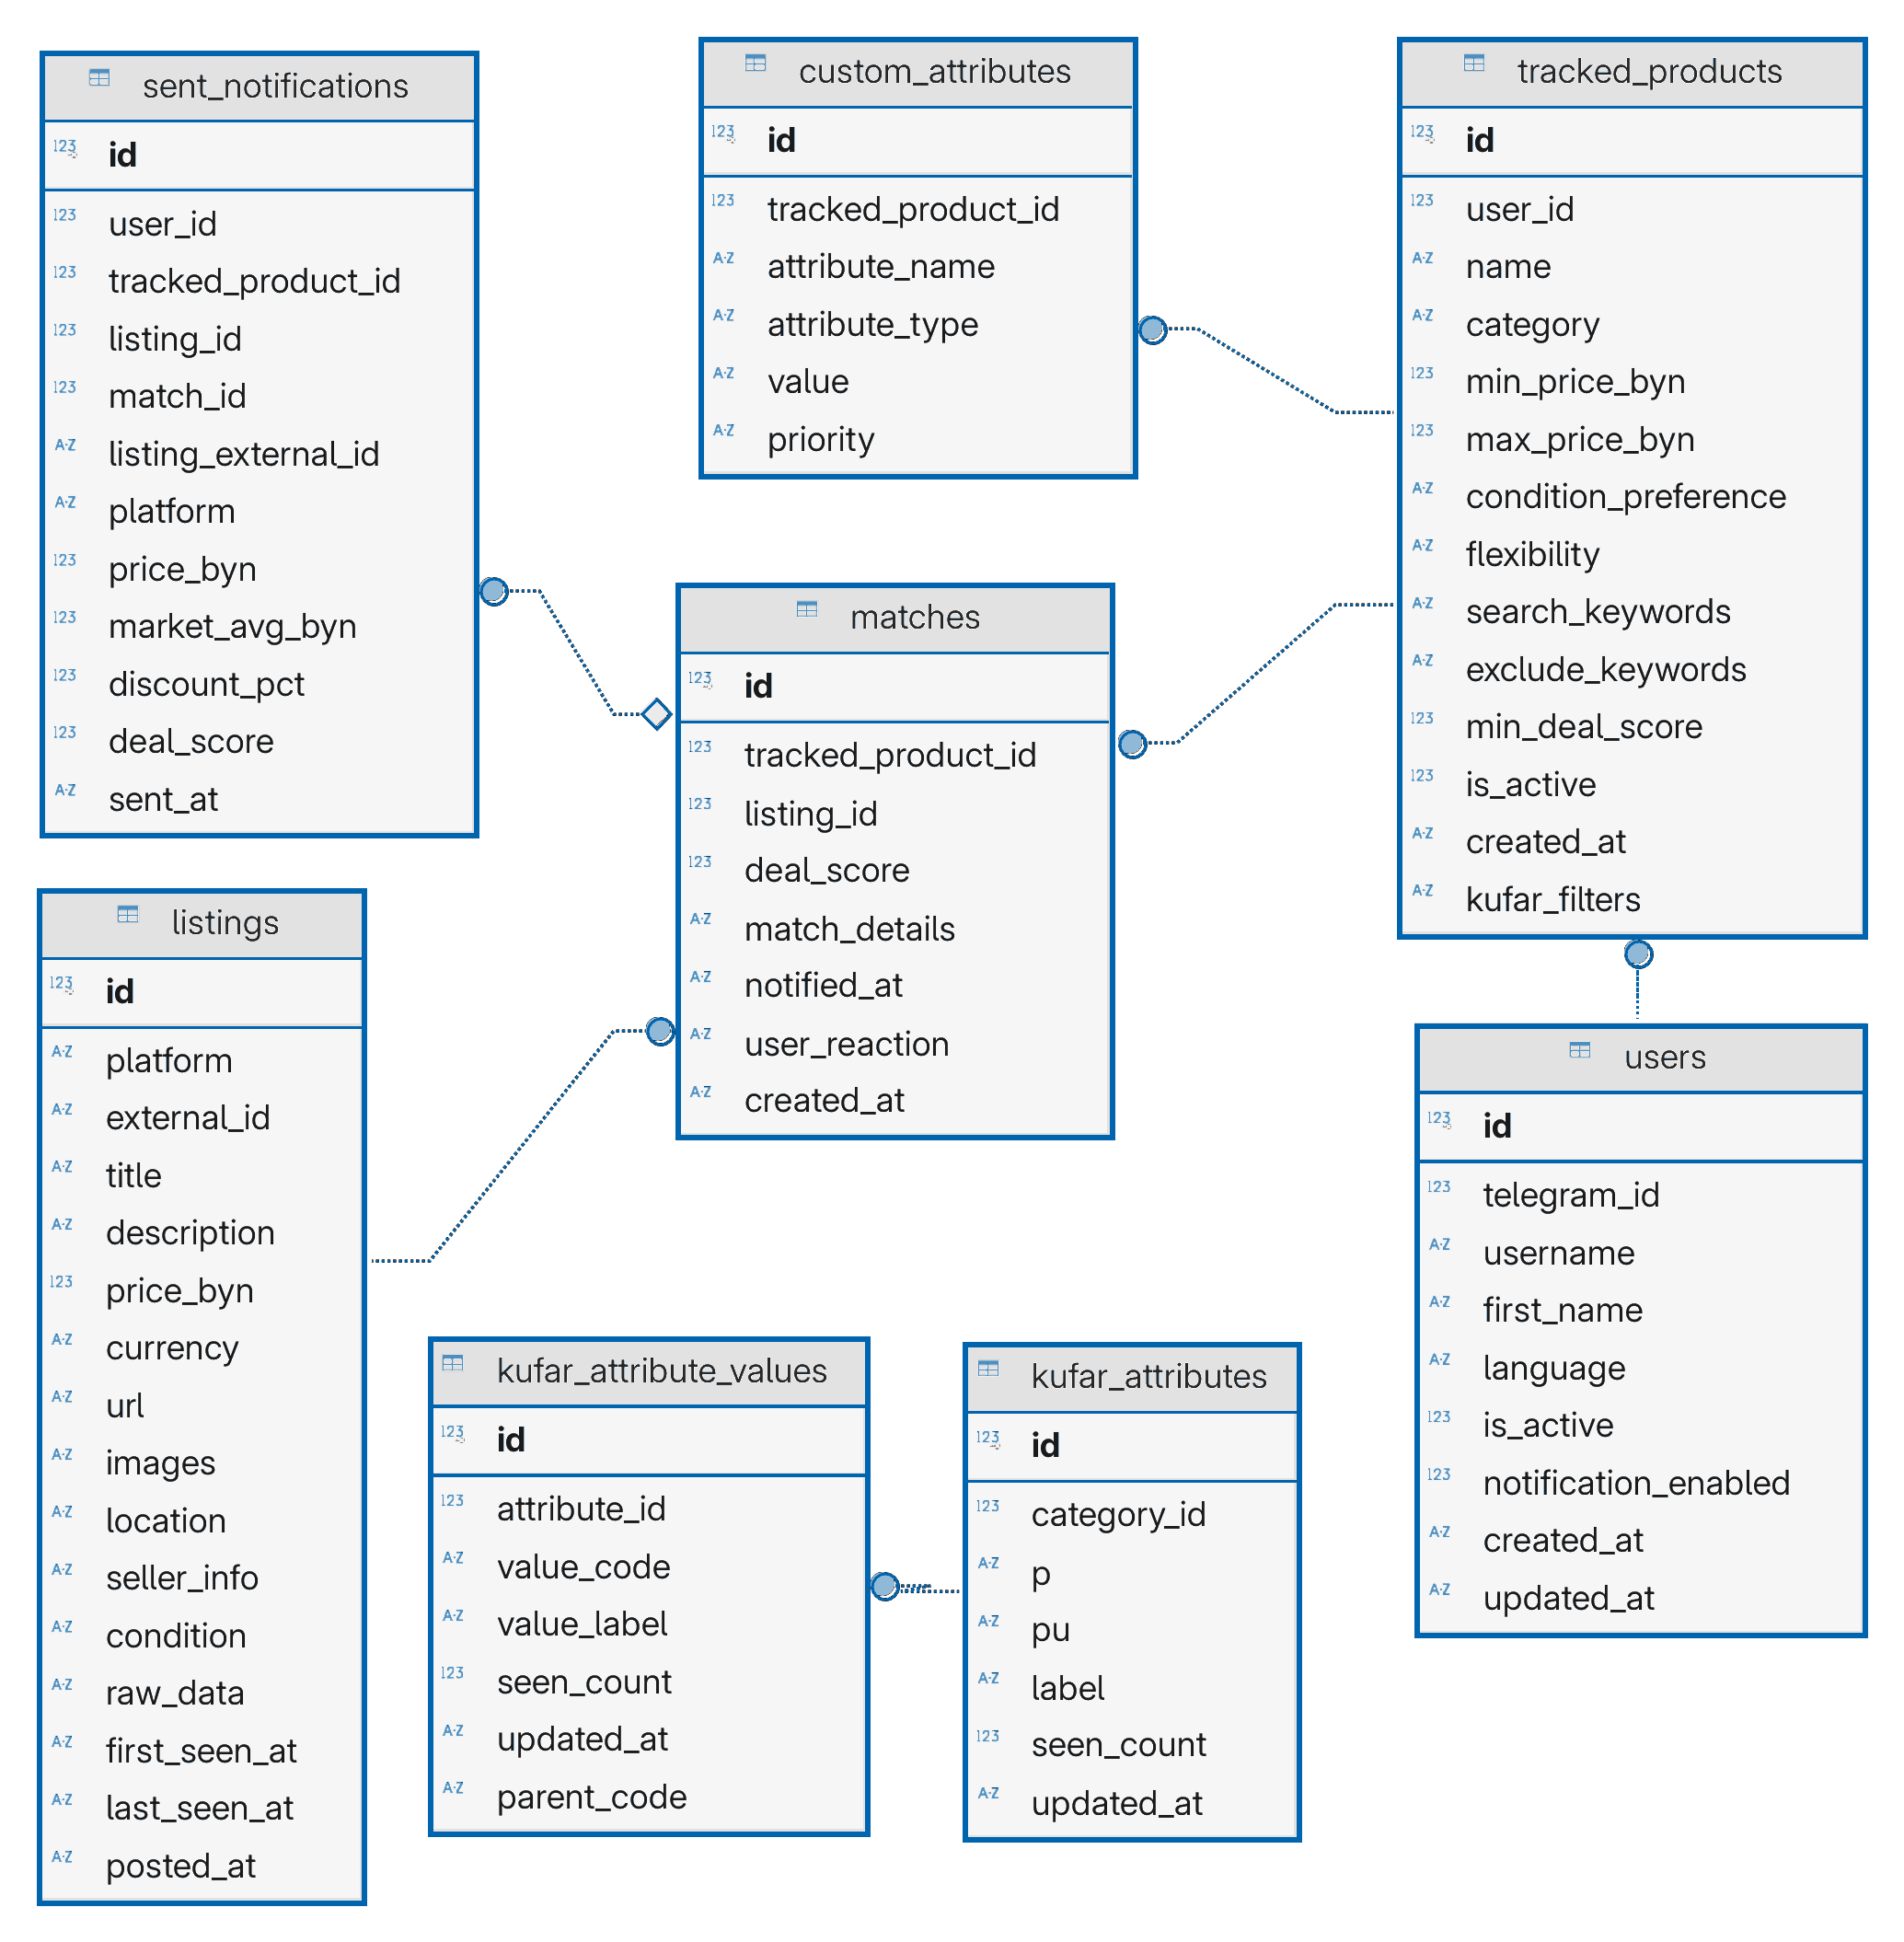
\includegraphics[width=\linewidth]{kufar/physical}
	\caption{Физическая схема базы данных}
	\label{fig:development:physical}
\end{figure}

\begin{table}[ht]
\caption{Таблицы базы данных}
\label{table:development:tables}
\centering
	\begin{tabular}{|>{\raggedright}m{0.27\textwidth}
	                |>{\raggedright}m{0.38\textwidth}
	                |>{\raggedright\arraybackslash}m{0.25\textwidth}|}
	\hline
	\centering Таблица & \centering Назначение & \centering\arraybackslash Рост \\
	\hline Пользователи & Учётные записи, настройки, электронная почта & По одной строке на пользователя \\
	\hline Отслеживаемые товары & Критерии поиска пользователей & Не более 25 строк \\
	\hline Объявления & Сведения, полученные с площадки & С каждым циклом опроса, очищается через 30 дней \\
	\hline Совпадения & Подошедшие объявления и очередь доставки & По мере отбора \\
	\hline Журнал уведомлений & Факты отправки с ценой & С каждой отправкой, очищается через 90 дней \\
	\hline Атрибуты фильтров & Характеристики категорий площадки & Пересобирается раз в неделю \\
	\hline Значения атрибутов & Возможные значения характеристик & Пересобирается раз в неделю \\
	\hline Пользовательские атрибуты & Резерв для расширения системы & Не заполняется \\
	\hline
	\end{tabular}
\end{table}

Типы данных выбраны по смыслу атрибутов. Первичными ключами всех таблиц служат целые числа с автоматическим приращением. Идентификатор пользователя \textit{Telegram} хранится 64-битным целым: значения таких идентификаторов уже выходят за пределы 32-битного типа. Строки с известной верхней границей длины, например имя, код характеристики или адрес электронной почты, хранятся в строковых полях ограниченной длины, до 255 символов. Заголовок, описание и ссылка объявления не имеют разумного предела и хранятся в текстовых полях без ограничения длины. Хеш кода подтверждения занимает ровно 64 символа, по длине шестнадцатеричной записи результата \textit{SHA-256}.

Цены хранятся числами с плавающей точкой двойной точности. В системе цены только сравниваются с порогом и между собой, а доля выгоды округляется до четырёх знаков, поэтому погрешность представления на результат не влияет. Если в систему будут добавлены суммирование или денежные расчёты, цены следует перевести в десятичный тип с фиксированной точностью.

Моменты времени хранятся без часового пояса и всегда в \textit{UTC}. Время публикации, которое площадка передаёт с указанием пояса, система приводит к \textit{UTC} перед записью. Благодаря этому сравнение «объявление опубликовано после добавления товара» корректно при любой настройке часового пояса сервера. Для дат создания и изменения записей значение по умолчанию задаёт сама СУБД текущим временем.

Поля с фиксированным набором значений (категория товара, площадка, реакция пользователя) объявлены перечислимыми типами \textit{PostgreSQL}. СУБД отклоняет любое значение вне перечня, и опечатка в коде не может записать в базу несуществующую категорию. Признаки хранятся логическим типом, а счётчики попыток целыми числами.

Тип \textit{JSON} использован в семи столбцах: обязательные слова, слова-исключения и фильтры площадки у товара, фотографии, продавец и исходный ответ у объявления, детали события у совпадения. У этих данных общее свойство: их всегда читают и записывают целиком и никогда не ищут в базе по отдельному элементу. Фильтры площадки, например, подставляются в запрос к \textit{Kufar.by} в неизменном виде.

\subsubsection{Нормализация}

Схема приведена к третьей нормальной форме с несколькими осознанными отступлениями.

Первая нормальная форма требует атомарности значений. Формально её нарушают \textit{JSON}-столбцы: список слов-исключений или набор фильтров хранится в одной ячейке. Вынесение их в отдельные таблицы дало бы одну-две лишние таблицы на каждый список и соединение при каждом чтении товара, но ни одного нового запроса, которому такая структура была бы нужна. Система не ищет товары по слову-исключению и не считает, сколько пользователей выбрали бренд. Когда такие запросы появятся, фильтры можно будет перенести в отдельную таблицу связи между товаром и значением атрибута без изменения остальной схемы.

Вторая нормальная форма выполняется автоматически: все таблицы имеют простой суррогатный первичный ключ, и частичной зависимости от части ключа возникнуть не может.

Третья нормальная форма требует, чтобы неключевые атрибуты не зависели друг от друга. Это требование намеренно нарушено в журнале уведомлений. Площадка, внешний идентификатор объявления и цена в нём дублируют данные таблицы объявлений. Дублирование сделано по двум причинам. Проверка повтора (отправлялось ли это объявление пользователю и по какой цене) выполняется для каждого уведомления, и без копии каждая такая проверка требовала бы соединения с таблицей объявлений. Кроме того, в журнале записана цена на момент отправки, а в таблице объявлений хранится текущая цена, которая со временем меняется. Это разные факты, поэтому формально зависимость отсутствует, хотя названия столбцов совпадают.

Данные подтверждения электронной почты (хеш кода, срок, число попыток) хранятся в таблице пользователей, хотя по смыслу образуют отдельный объект. Пользователь связан с ними отношением один к одному, данные невелики и всегда читаются вместе с пользователем, поэтому отдельная таблица только добавила бы соединение.

\subsubsection{Индексы}

Каждый индекс ускоряет чтение и замедляет запись: при вставке и обновлении строки СУБД перестраивает все индексы таблицы. Таблица объявлений обновляется на каждом цикле опроса, поэтому индексы подбирались не по столбцам, а по запросам, которые система действительно выполняет. Все индексы~-- сбалансированные деревья (\textit{B-tree}), принятые в \textit{PostgreSQL} по умолчанию: они обслуживают и поиск по равенству, и сравнение по диапазону, которое нужно при подсчёте уведомлений за период. Соответствие индексов запросам приведено в таблице~\ref{table:development:indexes}.

\begin{table}[ht]
\caption{Индексы и обслуживаемые ими запросы}
\label{table:development:indexes}
\centering
	\begin{tabular}{|>{\raggedright}m{0.3\textwidth}
	                |>{\raggedright}m{0.37\textwidth}
	                |>{\raggedright\arraybackslash}m{0.23\textwidth}|}
	\hline
	\centering Индекс & \centering Запрос & \centering\arraybackslash Частота \\
	\hline Объявления: площадка и внешний идентификатор (составной) & Поиск сохранённого объявления при обработке ответа площадки & До 1\,050 раз за цикл \\
	\hline Пользователи: идентификатор \textit{Telegram} (уникальный) & Определение пользователя по входящему сообщению & Каждое сообщение \\
	\hline Товары: владелец & Список товаров пользователя, подсчёт занятости личного лимита & Каждый диалог и каждое добавление \\
	\hline Совпадения: товар & Выборка очереди доставки, отчёт за период & Каждую минуту \\
	\hline Совпадения: объявление & Проверка, есть ли у объявления совпадения, при очистке & Раз в сутки \\
	\hline Журнал: получатель & Подсчёт уведомлений пользователя за сутки & Каждая отправка \\
	\hline Журнал: товар & Подсчёт уведомлений по товару за час & Каждая отправка \\
	\hline Журнал: внешний идентификатор объявления & Проверка, отправлялось ли объявление и по какой цене & Каждая отправка \\
	\hline Справочник: категория площадки, атрибут & Построение меню фильтров, обновление справочника & Каждое открытие фильтров \\
	\hline
	\end{tabular}
\end{table}

Самый частый запрос~-- поиск объявления по паре «площадка~-- внешний идентификатор». Поиск выполняется для каждого объявления в каждом цикле: при 25 товарах и 42 объявлениях на запрос это до 1\,050 поисков за цикл и более 500\,000 в сутки. Для него создан составной индекс по двум столбцам. До его появления на этих столбцах были только отдельные индексы, и планировщику запросов приходилось объединять их результаты. Порядок столбцов в составном индексе выбран так, чтобы индекс годился и для запросов по одной площадке: ведущим стоит столбец площадки, а внешний идентификатор уточняет запись внутри неё. Поскольку площадка в системе пока одна, отдельный индекс по ней стал избыточным: выборка не сужается, а запись замедляется, поэтому такой индекс можно удалить.

Уникальный индекс по идентификатору \textit{Telegram} решает две задачи сразу. Индекс поддерживает ограничение уникальности и обслуживает запрос, который выполняется чаще всех остальных запросов бота: на каждое входящее сообщение система находит пользователя по идентификатору его учётной записи. Без индекса этот поиск был бы последовательным просмотром всей таблицы пользователей.

Индекс по владельцу в таблице товаров обслуживает два запроса: вывод списка товаров пользователя и подсчёт занятости личного лимита перед добавлением нового товара. Оба выполняются с условием равенства по владельцу, и выборка по индексу возвращает сразу нужные несколько строк.

В таблице совпадений проиндексированы оба внешних ключа, но обслуживают они разные запросы. Индекс по товару соединяет совпадения с товарами при выборке очереди доставки и при формировании отчёта за период. Индекс по объявлению нужен задаче очистки: перед удалением устаревшего объявления система проверяет, не ссылается ли на него хотя бы одно совпадение, и без индекса такая проверка означала бы просмотр всей таблицы совпадений для каждого удаляемого объявления.

Три индекса журнала уведомлений поддерживают антиспам. По получателю считаются уведомления пользователя за текущие сутки, по товару~-- уведомления за последний час, по внешнему идентификатору объявления проверяется, отправлялось ли объявление этому пользователю и по какой цене. Все три запроса выполняются перед каждой отправкой, поэтому их стоимость напрямую влияет на длительность цикла доставки. Запрос проверки повтора отбирает строки по получателю, площадке и внешнему идентификатору одновременно; сейчас планировщик использует один из индексов и проверяет остальные условия по найденным строкам, а при росте журнала выгоднее станет составной индекс по получателю и внешнему идентификатору.

Справочник фильтров индексируется по категории площадки в таблице атрибутов и по атрибуту в таблице значений. Эти индексы обслуживают построение меню фильтров в боте, а уникальные ограничения на пару «категория~-- системное имя» и пару «атрибут~-- код значения» дополнительно ускоряют еженедельное обновление справочника: при повторном сборе система ищет существующую запись именно по этим парам.

Индексов по цене и категории в таблицах объявлений и товаров нет, и это сделано сознательно. Отбор объявлений по цене и категории выполняет сама площадка: система передаёт порог и категорию в поисковом запросе и получает только подходящие объявления. В базе данных по цене объявления не ищут. Таблица товаров содержит не более 25 строк, и последовательный просмотр такой таблицы быстрее обращения к индексу.

При росте нагрузки естественным улучшением станет частичный индекс по совпадениям, ещё не доставленным пользователю. Очередь доставки выбирает только их, а таких записей в любой момент единицы, тогда как в таблице совпадений хранится вся история. Частичный индекс занимает место, пропорциональное числу недоставленных совпадений, и не растёт вместе с историей.

\subsubsection{Ограничения целостности}

Целостность данных обеспечивается ограничениями на уровне СУБД и проверками на входе в серверный интерфейс.

На уровне СУБД действуют:
\begin{itemize}
	\item первичные ключи во всех таблицах;
	\item внешние ключи с явно заданными правилами удаления: товар ссылается на пользователя, совпадение на товар и объявление, запись журнала на пользователя, товар, объявление и совпадение, значение атрибута на атрибут;
	\item ограничения уникальности: идентификатор \textit{Telegram} пользователя, пара «категория~-- системное имя» у атрибута фильтра, пара «атрибут~-- код значения» у значения;
	\item ограничения \textit{NOT NULL} на всех обязательных столбцах; необязательными оставлены только данные, которых действительно может не быть: цена договорного объявления, адрес почты, время доставки недоставленного совпадения;
	\item перечислимые типы для категорий, площадок и реакций;
	\item значения по умолчанию на стороне СУБД для дат создания и изменения записей и для столбцов, добавленных миграциями; начальные значения признаков задаёт приложение при вставке записи.
\end{itemize}

Ограничения уникальности справочника позволяют пересобирать его без дублей: при повторном сборе существующее значение обновляется, а не добавляется второй раз. Совпадение для пары «товар~-- объявление» создаётся только после проверки, что такого совпадения ещё нет. Проверка и вставка выполняются в одной транзакции цикла опроса.

Удаление товара затрагивает зависимые записи, поэтому правило удаления задано в схеме для каждого внешнего ключа. Совпадения, пользовательские атрибуты и записи журнала уведомлений по товару удаляются вместе с ним (\textit{ON DELETE CASCADE}). Ссылка журнала на совпадение обнуляется (\textit{ON DELETE SET NULL}): запись журнала хранит собственную копию цены и внешнего идентификатора объявления и без совпадения не теряет смысла. По тому же правилу вместе с пользователем удаляются его товары и журнал, а вместе с атрибутом фильтра~-- его значения. У ссылки журнала на объявление правила удаления нет: очистка удаляет только объявления без совпадений, а на них журнал не ссылается. Правила выполняет сама СУБД, поэтому одного запроса \textit{DELETE} к таблице товаров достаточно, чтобы удалить товар со всеми зависимыми записями в одной транзакции.

Проверки, которые неудобно выразить ограничениями СУБД, выполняются при приёме данных серверным интерфейсом: пороговая цена больше нуля и не больше 10~000~000 рублей, название не длиннее 255 символов, не более 20 слов в каждом списке и не более 100 символов в слове, коды фильтров принадлежат категории товара. Файл \textit{CSV} при импорте ограничен 256~КБ и 100 строками. Некорректный запрос отклоняется с понятным сообщением до обращения к базе данных.

Каждый запрос к серверному интерфейсу выполняется в одной транзакции: при успехе изменения фиксируются, при любой ошибке транзакция откатывается целиком. Цикл опроса площадки записывает объявления и совпадения всех товаров одной транзакцией. Доставка уведомлений отмечает совпадение доставленным и добавляет запись в журнал в одной транзакции, поэтому отметка без записи или запись без отметки появиться не могут.

\subsubsection{Миграции и обслуживание данных}

Схема базы данных изменялась пятью миграциями. Первая создаёт все таблицы и индексы. Вторая добавляет в таблицу совпадений счётчик попыток доставки и текст ошибки, на которых построена повторная отправка. Третья добавляет составной индекс по площадке и внешнему идентификатору объявления. Четвёртая добавляет поля электронной почты в таблицу пользователей и отдельную почтовую очередь в таблицу совпадений. Пятая задаёт правила удаления для внешних ключей и удаляет избыточный индекс по площадке. Новые обязательные столбцы добавлялись со значением по умолчанию на стороне СУБД, поэтому миграции применялись к таблицам, уже содержащим данные, без их пересоздания.

Миграции применяет серверный сервис при запуске. Перед применением сервис берёт рекомендательную блокировку \textit{PostgreSQL}: если одновременно запускаются два экземпляра сервиса, второй дожидается, пока первый закончит миграцию, и находит схему уже в актуальном состоянии.

Объявления сохраняются на каждом цикле опроса, и без очистки их таблица росла бы всё время работы системы. Раз в сутки удаляются объявления, которые не появлялись в выдаче 30 дней и не участвуют ни в одном совпадении. Объявления с совпадениями сохраняются, потому что на них ссылается история уведомлений и отчёты пользователя. Записи журнала уведомлений старше 90 дней удаляются по тому же расписанию.

\subsubsection{Резервное копирование}

Резервное копирование выполняет отдельный контейнер. Раз в сутки контейнер создаёт полный логический дамп базы данных утилитой \textit{pg\_dump}, сжимает его и сохраняет в каталог на сервере вне тома СУБД. Хранятся семь последних копий, более старые удаляются автоматически.

Резервная копия, которую ни разу не восстанавливали, не даёт гарантии, что данные удастся вернуть. Поэтому в систему входит сценарий проверки восстановления. Сценарий создаёт временную базу данных, загружает в неё последний дамп, подсчитывает строки в основных таблицах и удаляет временную базу. Проверка запускается вручную одной командой и не затрагивает рабочую базу.

Данные СУБД хранятся в именованном томе \textit{Docker}. Пересборка и перезапуск контейнеров их не затрагивают, а резервные копии в отдельном каталоге защищают от повреждения самого тома.


\subsection{Применение интеллектуальных инструментов в инженерном проектировании}
\label{sec:development:ai}

Под интеллектуальными инструментами здесь понимаются большие языковые модели, которые принимают постановку задачи на естественном языке и возвращают текст, код или описание схемы. При разработке системы применялась модель \textit{Claude} в среде \textit{Claude Code}, работающая с файлами проекта. Инструмент использовался как помощник на трёх этапах: при проектировании модели данных, при написании кода и при подготовке графического материала. Решение о применении каждого предложенного варианта принимал разработчик после проверки.

\subsubsection{Порядок работы с инструментом}

Работа строилась по одной схеме. Задача формулировалась вместе с контекстом: фрагментом схемы базы данных, текстом запроса или сообщением об ошибке. Полученный ответ не принимался как готовый результат, а проверялся: код~-- запуском тестов, запросы~-- планом выполнения, схема данных~-- сверкой с требованиями подраздела~\ref{sec:analysis:specification}. Ответы, которые не удавалось воспроизвести или обосновать, отбрасывались.

Такой порядок выбран из-за особенности инструмента: модель порождает синтаксически верный и правдоподобный результат, но не проверяет его на данных системы. Ошибка в ответе выглядит так же убедительно, как верное решение, поэтому проверка обязательна для каждого предложения.

\subsubsection{Решённые задачи}

Задачи, при решении которых применялся инструмент, сведены в таблицу~\ref{table:development:ai}.

\begin{table}[ht]
\caption{Задачи, решённые с применением интеллектуальных инструментов}
\label{table:development:ai}
\centering
	\begin{tabular}{|>{\raggedright}m{0.26\textwidth}
	                |>{\raggedright}m{0.31\textwidth}
	                |>{\raggedright\arraybackslash}m{0.31\textwidth}|}
	\hline
	\centering Задача & \centering Результат работы инструмента & \centering\arraybackslash Что потребовало проверки \\
	\hline Проектирование модели данных & Черновой состав сущностей и связей по словесному описанию предметной области & Мощность связей, состав ключей, выделение совпадения в отдельную сущность \\
	\hline Подбор индексов & Перечень индексов под запросы цикла опроса & Соответствие плану выполнения запроса, поиск избыточных индексов \\
	\hline Разбор ответа площадки & Черновой код разбора полей объявления и характеристик категории & Поведение на объявлениях без цены и без описания \\
	\hline Миграции схемы & Заготовки миграций с прямым и обратным переходом & Правила удаления связанных записей, порядок применения \\
	\hline Тесты & Наборы проверок для отбора объявлений и лимитов уведомлений & Полнота граничных случаев \\
	\hline Графический материал & Исходные описания схем и диаграмм для \textit{Graphviz} и \textit{PlantUML} & Соответствие ГОСТ~19.701–90 и фактическому коду \\
	\hline
	\end{tabular}
\end{table}

\subsubsection{Ошибки, найденные при проверке}

Проверка результатов выявила два дефекта, которые относятся непосредственно к базе данных и были исправлены отдельными миграциями.

1. Правила удаления связанных записей существовали только в коде приложения, а в схеме базы данных отсутствовали. Удаление товара, по которому уже отправлено уведомление, завершалось нарушением ссылочной целостности. Миграция добавила правила в саму схему: для товаров, совпадений и значений справочника задано каскадное удаление, а ссылка журнала на совпадение обнуляется, поскольку запись журнала хранит собственную копию цены и идентификатора объявления и должна пережить удаление совпадения.

2. Среди индексов таблицы объявлений оказался избыточный: отдельный индекс по площадке дублировал составной индекс по паре «площадка~-- внешний идентификатор», который начинается с того же столбца и обслуживает те же запросы. Избыточный индекс удалён, потому что он замедлял вставку объявлений и занимал место, не ускоряя ни один запрос.

Оба дефекта не были обнаружены ни тестами, ни разбором кода: первый проявляется только при удалении товара с историей уведомлений, второй вообще не влияет на правильность результата. Нашла их сверка схемы с перечнем запросов цикла, выполненная вручную.

\subsubsection{Оценка применимости}

Инструмент даёт выигрыш на задачах, где ответ проверяется быстро и однозначно: черновик кода разбора ответа площадки, заготовка миграции, набор тестов, описание диаграммы для \textit{Graphviz}. Время на такие задачи сокращается заметно, потому что проверка занимает меньше времени, чем написание с нуля.

На задачах, где решение зависит от особенностей площадки и характера нагрузки, выигрыш оказался небольшим. Ограничение частоты запросов, стратегия пауз после отказа площадки, порог выгодности и правила повторной отправки уведомления подбирались по наблюдениям за работой системы, а не по предложенному варианту. Модель не располагает сведениями о поведении конкретной площадки и о распределении цен в категориях, поэтому её предложения в этой части оставались общими.

Отсюда следует правило, которого придерживались при разработке: интеллектуальный инструмент применим там, где результат проверяем формально, и не применим там, где решение опирается на данные, которых у инструмента нет. Ответственность за принятое решение остаётся на разработчике в обоих случаях.


\subsection{Программная реализация системы}
\label{sec:development:implementation}

\subsubsection{Архитектура системы}

Система состоит из нескольких сервисов, каждый из которых запущен в отдельном контейнере на одном сервере. Архитектура развёртывания приведена на рисунке~\ref{fig:development:architecture}.

\begin{figure}[H]
	\centering
	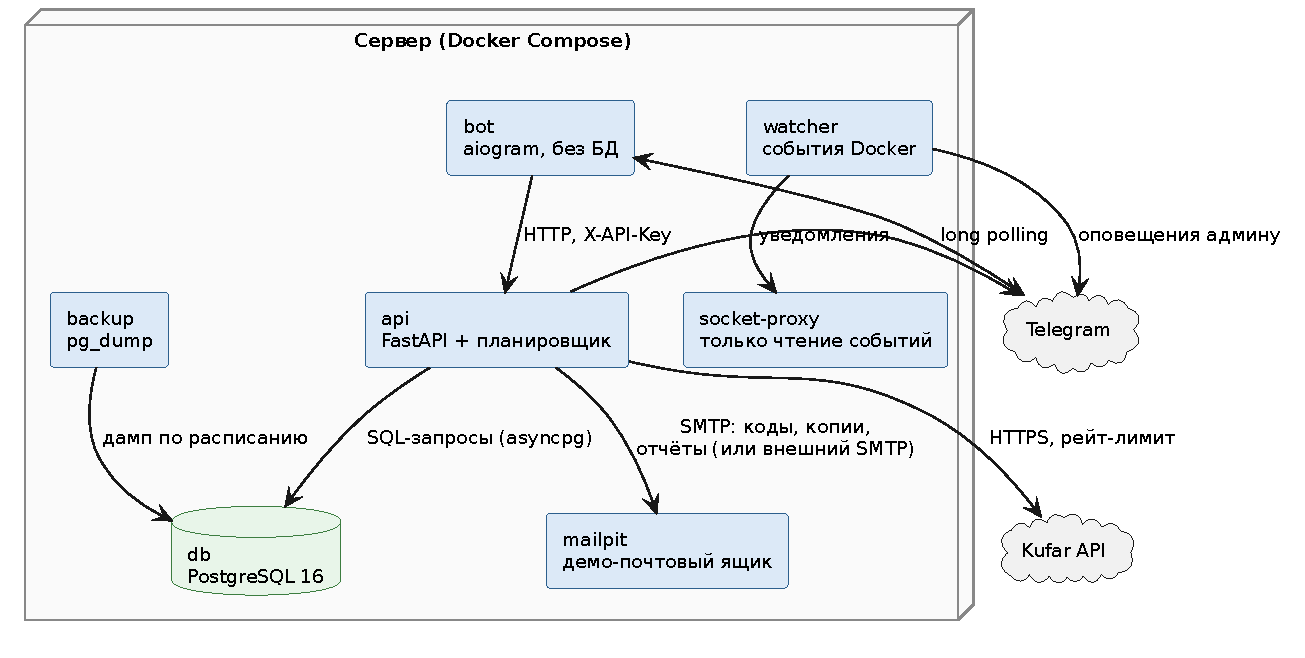
\includegraphics[width=\linewidth]{kufar/architecture}
	\caption{Архитектура развёртывания системы}
	\label{fig:development:architecture}
\end{figure}

Основную работу выполняют три сервиса. СУБД \textit{PostgreSQL} хранит все данные. Серверный сервис владеет базой данных: только этот сервис выполняет SQL-запросы, применяет миграции и запускает периодические задачи. Бот отвечает только за диалог с пользователем в \textit{Telegram}. Собственного доступа к базе данных у бота нет: все данные для показа и изменения бот получает от серверного сервиса по \textit{HTTP}, прикладывая к каждому запросу общий секретный ключ.

Такое разделение выбрано ради данных. Когда в базу пишет только один сервис, все правила записи собраны в одном месте. Лимит отслеживаемых товаров, например, проверяется в серверном сервисе, и обойти его нельзя ни через бот, ни через импорт файла, ни прямым запросом к интерфейсу. Схемой базы данных управляет тот же сервис, поэтому несогласованных изменений структуры не бывает.

Уведомления серверный сервис отправляет в \textit{Telegram} сам, не через бота. Для отправки сообщений достаточно токена бота, а получать входящие сообщения продолжает сервис бота. Поэтому остановка бота, например при обновлении, не прерывает доставку уведомлений.

Вспомогательные сервисы обеспечивают надёжность. Сервис резервного копирования раз в сутки выгружает дамп базы. Служба мониторинга следит за событиями контейнеров и сообщает администратору о запуске, падении и потере работоспособности любого из них. События \textit{Docker} служба читает через отдельный посредник, который открывает к ним доступ только на чтение: прямой доступ к управляющему сокету \textit{Docker} равносилен правам администратора сервера. Почтовый сервер-ловушка принимает все письма системы и показывает их в веб-интерфейсе, что упрощает проверку почтовых функций без настоящего почтового ящика.

Внутри серверного сервиса код разделён на слои. Модули обработки и их связи с сущностями данных показаны на рисунке~\ref{fig:development:classes:logic}.

Сущности данных описывают содержимое таблиц базы данных:
\begin{itemize}
	\item \textit{User}~-- пользователь: номер учётной записи \textit{Telegram}, язык интерфейса, признаки активности и уведомлений, адрес электронной почты и признак его подтверждения;
	\item \textit{TrackedProduct}~-- отслеживаемый товар: название, категория, границы цены, списки слов поиска и исключений, фильтры площадки в поле \textit{kufar\_filters} и порог выгодности \textit{min\_deal\_score};
	\item \textit{Listing}~-- объявление, полученное с площадки: площадка, внешний идентификатор, заголовок, описание, цена, ссылка, время публикации, время первого и последнего появления в выдаче;
	\item \textit{Match}~-- совпадение объявления с отслеживаемым товаром: показатель выгоды, подробности отбора, время доставки \textit{notified\_at}, число попыток \textit{notify\_attempts} и текст ошибки;
	\item \textit{SentNotification}~-- запись журнала отправленных уведомлений с ценой объявления на момент отправки;
	\item \textit{KufarAttribute} и \textit{KufarAttributeValue}~-- справочник характеристик категорий площадки и их допустимых значений.
\end{itemize}

Доступ к площадке построен на наследовании. Абстрактный класс \textit{BaseScraper} хранит сетевую сессию, удерживает частоту запросов методом \textit{\_rate\_limit} и выполняет запрос методом \textit{\_get}, а поиск и загрузку отдельного объявления объявляет, но не реализует. Класс \textit{KufarScraper} реализует их для \textit{Kufar.by}: метод \textit{\_build\_params} собирает параметры запроса по стратегии категории, методы \textit{\_parse\_search\_response} и \textit{\_parse\_ad} превращают ответ площадки в структуры \textit{ScrapedListing}. Добавление второй площадки сводится к новому наследнику \textit{BaseScraper}, потому что остальной код работает со структурой \textit{ScrapedListing} и об устройстве площадки ничего не знает.

Обработка данных вынесена в отдельные модули и классы, показанные на рисунке~\ref{fig:development:classes:logic}.

\begin{figure}[H]
	\centering
	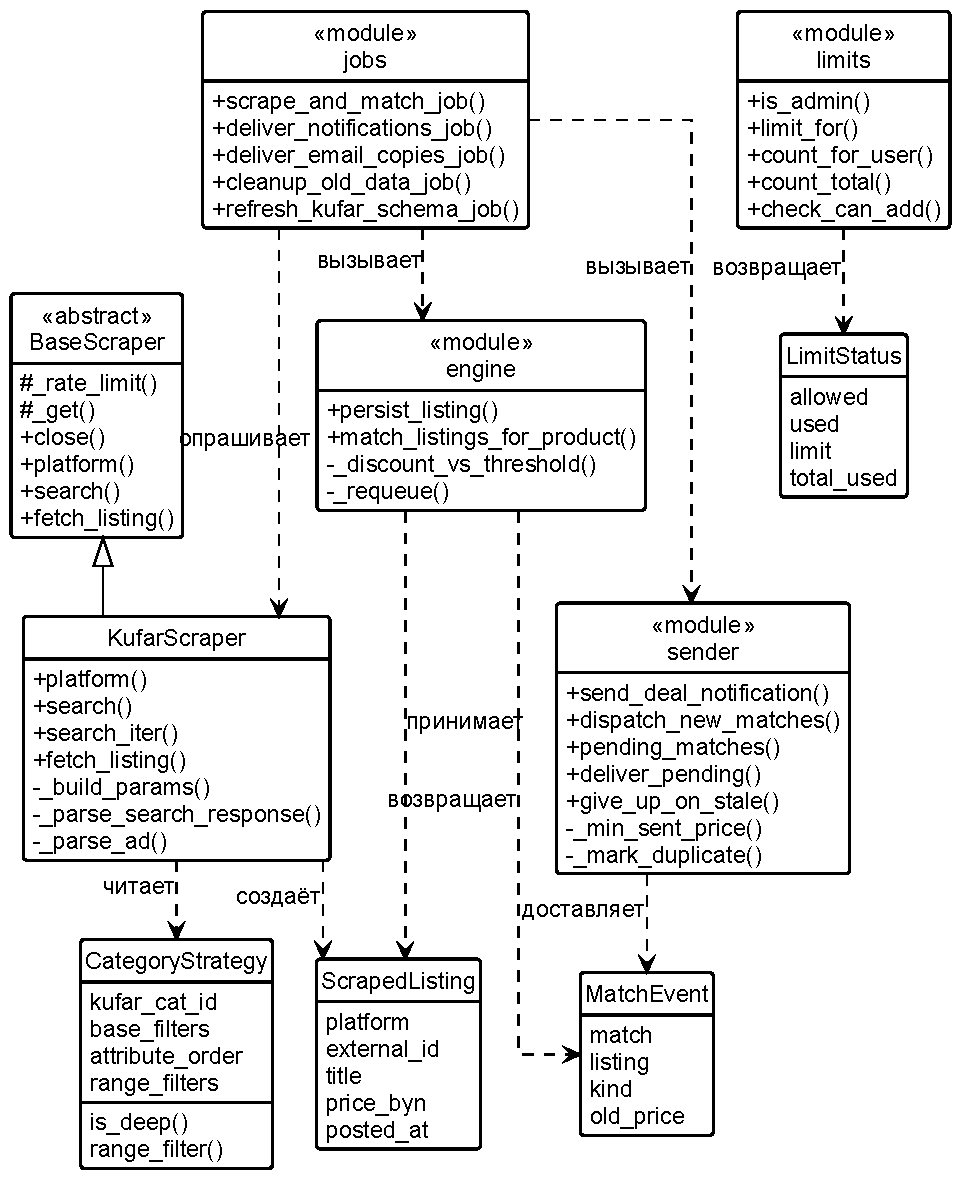
\includegraphics[width=\linewidth]{kufar/classes_logic}
	\caption{Диаграмма классов модулей обработки}
	\label{fig:development:classes:logic}
\end{figure}

Назначение модулей:
\begin{itemize}
	\item \textit{engine}~-- функция \textit{persist\_listing} добавляет или обновляет объявление и возвращает прежнюю цену, функция \textit{match\_listings\_for\_product} отбирает объявления по критериям товара, создаёт совпадения и возвращает список событий \textit{MatchEvent};
	\item \textit{sender}~-- функция \textit{deliver\_pending} разбирает очередь недоставленных совпадений, функция \textit{send\_deal\_notification} отправляет одно уведомление, функция \textit{\_min\_sent\_price} проверяет журнал на повтор, функция \textit{give\_up\_on\_stale} закрывает совпадения старше трёх суток;
	\item \textit{limits}~-- функция \textit{check\_can\_add} проверяет лимит отслеживаемых товаров и возвращает структуру \textit{LimitStatus}, функции \textit{is\_admin} и \textit{limit\_for} определяют потолок для конкретного пользователя;
	\item \textit{jobs}~-- периодические задачи планировщика: опрос площадки \textit{scrape\_and\_match\_job}, доставка уведомлений \textit{deliver\_notifications\_job}, почтовые копии \textit{deliver\_email\_copies\_job}, очистка устаревших данных \textit{cleanup\_old\_data\_job} и обновление справочника \textit{refresh\_kufar\_schema\_job}.
\end{itemize}

В структуре \textit{CategoryStrategy} собраны правила отбора для каждой категории: код категории площадки, обязательные фильтры, порядок характеристик и их числовые диапазоны. Результаты работы модули передают друг другу структурами: \textit{ScrapedListing}~-- разобранное объявление площадки, \textit{MatchEvent}~-- найденное совпадение вместе с прежней ценой и типом события, \textit{LimitStatus}~-- результат проверки лимита. На диаграммах не показаны части системы, которые не работают с данными напрямую: обработчики бота, маршруты программного интерфейса, словари локализации и формирование книг \textit{Excel}.

Слои обращаются друг к другу сверху вниз. Маршрут программного интерфейса проверяет входные данные и вызывает сервис бизнес-логики. Сервис выполняет SQL-запросы к базе данных и возвращает результат. Модуль \textit{jobs} обращается к тем же модулям \textit{engine}, \textit{sender} и \textit{limits}, что и маршруты, поэтому одно и то же правило, например проверка повтора уведомления, реализовано один раз. Класс \textit{KufarScraper} о базе данных ничего не знает и возвращает объявления структурами \textit{ScrapedListing}, а сохраняет их функция \textit{persist\_listing}.

\subsubsection{Цикл опроса площадки и обработка объявлений}

Цикл опроса запускается планировщиком каждые 3 минуты. Одновременно может выполняться только один цикл: если предыдущий ещё не завершился, следующий запуск пропускается. Цикл выполняет следующие шаги:
\begin{enumerate}
	\item Проверить паузу. Если после отказа площадки ещё остались пропускаемые циклы, уменьшить их счётчик и завершить цикл.
	\item Выбрать из базы данных все активные отслеживаемые товары.
	\item Для каждого товара по очереди:
	\begin{itemize}[itemindent=2.2ex,leftmargin=2\parindent,label=--]
		\item пропустить товар, если у него не задана пороговая цена;
		\item по стратегии категории сформировать запрос: код категории площадки, тип сделки, обязательные фильтры, фильтры пользователя, название и ограничение цены сверху, равное порогу;
		\item дождаться разрешения ограничителя частоты и отправить запрос;
		\item если площадка ответила кодом 403 или 429, прервать цикл целиком;
		\item передать полученные объявления модулю отбора.
	\end{itemize}
	\item Зафиксировать транзакцию.
	\item Если цикл занял больше 80\,\% интервала, записать предупреждение в журнал работы.
\end{enumerate}

Ограничитель частоты работает в два слоя. Перед каждым запросом выдерживается пауза около 2 секунд со случайной добавкой от 0,5 до 1,5 секунды, чтобы запросы не шли с одинаковым интервалом. Кроме того, ограничитель помнит время запросов за последнюю минуту и, если их уже 30, ждёт, пока самый старый выйдет из этого окна. При отказе площадки пауза до следующего опроса удваивается с каждым отказом подряд: 1, 2, 4, 8, 16 циклов. Администратор получает одно оповещение, а повторные оповещения того же вида в течение 30 минут подавляются.

Модуль отбора обрабатывает каждое полученное объявление так:
\begin{enumerate}
	\item Найти объявление в базе данных по паре «площадка~-- внешний идентификатор».
	\item Если объявление найдено, запомнить его прежнюю цену и обновить запись новыми данными, иначе добавить новую запись.
	\item Проверить релевантность. Объявление отклоняется, если выполняется хотя бы одно условие:
	\begin{itemize}[itemindent=2.2ex,leftmargin=2\parindent,label=--]
		\item цена отсутствует, не ниже порога или ниже минимальной правдоподобной цены категории;
		\item заголовок содержит стоп-слово категории (для электроники это «чехол», «защитное стекло» и подобные);
		\item заголовок или описание содержат слово-исключение пользователя;
		\item в заголовке или описании нет какого-либо слова из названия товара (в категориях с фильтрами площадки проверка названия не выполняется);
		\item нет какого-либо обязательного слова.
	\end{itemize}
	\item Если совпадение для этой пары «товар~-- объявление» уже есть, обновить его только при снижении цены.
	\item Иначе определить тип события: «новое», если объявление опубликовано после добавления товара, «снижение цены», если цена упала с прошлого опроса. Если ни то ни другое, объявление пропускается.
	\item Создать совпадение с показателем выгоды и пустым временем доставки.
\end{enumerate}

Проверка названия допускает расхождения в написании. Слово из названия ищется в три этапа: сначала как подстрока текста объявления, затем по словарю известных вариантов записи (латиница и кириллица, распространённые сокращения), затем нечётким сравнением с каждым словом текста. На последнем этапе слово длиной от трёх символов считается найденным, если мера сходства на основе редакционного расстояния составляет не менее 85\,\%.

Отдельно работает мгновенный поиск. Сразу после добавления товара система выполняет тот же запрос к площадке и те же проверки релевантности, сортирует прошедшие объявления по цене и показывает пользователю пять самых дешёвых. В базу данных эти объявления не записываются: мгновенный поиск показывает состояние рынка, а отслеживание начинается с момента добавления товара.

\subsubsection{Механизм доставки уведомлений}

Уведомления доставляются по схеме исходящей очереди (\textit{outbox}). Цикл опроса только записывает совпадения в базу данных, а отправляет их отдельная задача, которую планировщик запускает каждую минуту. Очередью служит сама таблица совпадений: в очереди находятся записи с пустым временем доставки. Отдельной таблицы или брокера сообщений для этого не нужно: запись совпадения и постановка в очередь выполняются одной операцией в одной транзакции.

Задача доставки выполняет следующие шаги:
\begin{enumerate}
	\item Выбрать до 50 совпадений в порядке создания, для которых одновременно:
	\begin{itemize}[itemindent=2.2ex,leftmargin=2\parindent,label=--]
		\item время доставки пусто;
		\item неудачных попыток меньше пяти;
		\item совпадение создано не раньше трёх суток назад;
		\item товар активен, пользователь активен и не отключил уведомления.
	\end{itemize}
	\item Сгруппировать совпадения по товарам.
	\item Для каждого товара посчитать, сколько уведомлений ещё можно отправить: не больше пяти за последний час по этому товару и не больше 30 за текущие сутки пользователю. Если лимит исчерпан, оставить совпадения в очереди.
	\item Отсортировать совпадения товара по цене, чтобы при ограниченном лимите первыми ушли самые выгодные.
	\item Для каждого совпадения найти в журнале минимальную цену, по которой это объявление уже отправлялось пользователю:
	\begin{itemize}[itemindent=2.2ex,leftmargin=2\parindent,label=--]
		\item если такой отправки не было, отправить уведомление;
		\item если новая цена ниже минимальной, отправить уведомление с пометкой о снижении цены;
		\item иначе закрыть совпадение как дубликат.
	\end{itemize}
	\item После успешной отправки заполнить время доставки и добавить запись в журнал уведомлений.
	\item Зафиксировать транзакцию.
\end{enumerate}

Ошибки отправки обрабатываются по-разному. Если \textit{Telegram} просит снизить частоту запросов, доставка прекращается до следующего запуска: это ограничение действует на бота целиком, и продолжать отправку другим пользователям бессмысленно. Пользователь, заблокировавший бота, помечается неактивным, и его совпадения перестают выбираться из очереди. При любой другой ошибке у совпадения увеличивается счётчик попыток и сохраняется текст ошибки, а само совпадение остаётся в очереди до следующего запуска. После пятой неудачной попытки совпадение из очереди исключается, а число таких совпадений записывается в журнал работы.

Почтовые копии ведут отдельную очередь в той же таблице совпадений, со своим временем отправки и счётчиком попыток. Копия отправляется только для совпадения, уже доставленного в \textit{Telegram}, поэтому все проверки лимитов и повторов действуют и для почты. Раз в 5 минут задача собирает все новые доставленные совпадения пользователя, у которого подтверждён адрес и включены копии, и отправляет одно сводное письмо со списком до 20 объявлений. Сбой почтового сервера не задерживает доставку в \textit{Telegram}, потому что две очереди обрабатываются разными задачами.

\subsubsection{Лимиты отслеживания и права администратора}

Каждый отслеживаемый товар добавляет один запрос к площадке за цикл опроса, поэтому число товаров ограничено двумя пределами:
\begin{itemize}
	\item личный лимит: 3 товара для пользователя и 10 для администратора;
	\item общий лимит: не более 25 товаров на всю систему.
\end{itemize}

Личный лимит защищает от ситуации, когда один пользователь занимает всю систему. Общий лимит защищает площадку и саму систему: при интервале опроса 180 секунд и примерно 3 секундах на запрос с учётом паузы за цикл можно обработать около 60 товаров. Предел в 25 товаров оставляет запас, чтобы цикл гарантированно завершался до начала следующего. При запуске серверный сервис сравнивает общий лимит с этой расчётной ёмкостью и предупреждает в журнале работы, если лимит задан больше, чем цикл успевает обработать.

Проверка лимитов выполняется дважды: перед началом диалога добавления товара и в момент сохранения. Вторая проверка нужна потому, что за время диалога другой пользователь мог занять последнее свободное место. Логика проверки такова:
\begin{enumerate}
	\item Посчитать товары пользователя и товары всех пользователей.
	\item Если товаров пользователя не меньше его личного лимита, отказать с пояснением «достигнут личный лимит».
	\item Если товаров в системе не меньше 25, отказать с пояснением «достигнут общий лимит системы».
	\item Иначе разрешить добавление.
\end{enumerate}

Все пути добавления товара проходят через одну и ту же операцию сервиса товаров: пошаговый диалог, импорт из ссылки и импорт файла \textit{CSV}. При импорте файла товары добавляются по строкам, пока лимит не исчерпан. В отчёте об импорте пользователь видит число добавленных товаров, ошибки по номерам строк и сообщение о том, какой лимит остановил импорт.

Права администратора определяются списком идентификаторов \textit{Telegram} в конфигурации системы, отдельной таблицы ролей нет. Администраторов в системе единицы, и назначает их владелец сервера, изменяя конфигурацию. Администратор отличается от пользователя тремя возможностями: личным лимитом в 10 товаров, отчётом о состоянии системы и служебными оповещениями о блокировке со стороны площадки и о событиях контейнеров. Остальные функции у него те же, что у пользователя, и доступа к чужим товарам администратор не получает: любая операция с товаром выполняется только в пределах товаров владельца.



	\section{Руководство пользователя}
\label{sec:manual}

Для работы с системой не нужно устанавливать отдельное приложение: достаточно клиента \textit{Telegram} на смартфоне, компьютере или в браузере. Пользователь находит бота по имени и отправляет команду /\textit{start}. Отдельной регистрации нет. При первом сообщении система сама создаёт учётную запись по идентификатору \textit{Telegram}, а язык интерфейса выбирает по языку приложения \textit{Telegram}: русский или английский.

В ответ на команду /\textit{start} бот присылает приветствие с кратким описанием работы и кнопки главного меню: «Мои товары», «Добавить товар», «Настройки» и «Помощь». Те же четыре кнопки закрепляются под полем ввода сообщения, так что главное меню доступно на любом экране. Главное меню показано на рисунке~\ref{fig:manual:start}.

\begin{figure}[H]
	\centering
	
\includegraphics[scale=0.6]{kufar/screens/start.png}
	\caption{Приветствие и главное меню бота}
	\label{fig:manual:start}
\end{figure}

Кроме кнопок, бот понимает команды: /\textit{start}~-- главное меню, /\textit{add}~-- добавить товар, /\textit{my}~-- мои товары, /\textit{report}~-- отчёт в \textit{Excel}, /\textit{settings}~-- настройки, /\textit{language}~-- язык интерфейса, /\textit{profile}~-- профиль, /\textit{help}~-- справка. Список команд продублирован в меню \textit{Telegram} слева от поля ввода.

\subsection{Роль администратора}
\label{sec:manual:admin}

Администратор~-- пользователь, идентификатор \textit{Telegram} которого указан в конфигурации системы. Отдельного входа или пароля у администратора нет: бот распознаёт его по учётной записи \textit{Telegram}. Чтобы назначить администратора, владелец сервера добавляет его идентификатор в список администраторов в файле окружения и перезапускает сервисы. Узнать свой идентификатор можно в разделе профиля бота.

Администратор пользуется всеми функциями пользователя, описанными в подразделе~\ref{sec:manual:user}. Возможности администратора отличаются в трёх местах.

\subsubsection{Повышенный лимит отслеживания}

Администратор может отслеживать до 10 товаров вместо 3. В профиле (команда /\textit{profile}) в строке «Статус» указано «администратор», а в строке «Лимит отслеживания» видно, сколько товаров занято у него самого и во всей системе. Общий предел в 25 товаров действует и для администратора и защищает площадку от перегрузки запросами. Профиль администратора показан на рисунке~\ref{fig:manual:admin_profile}.

\begin{figure}[H]
	\centering
	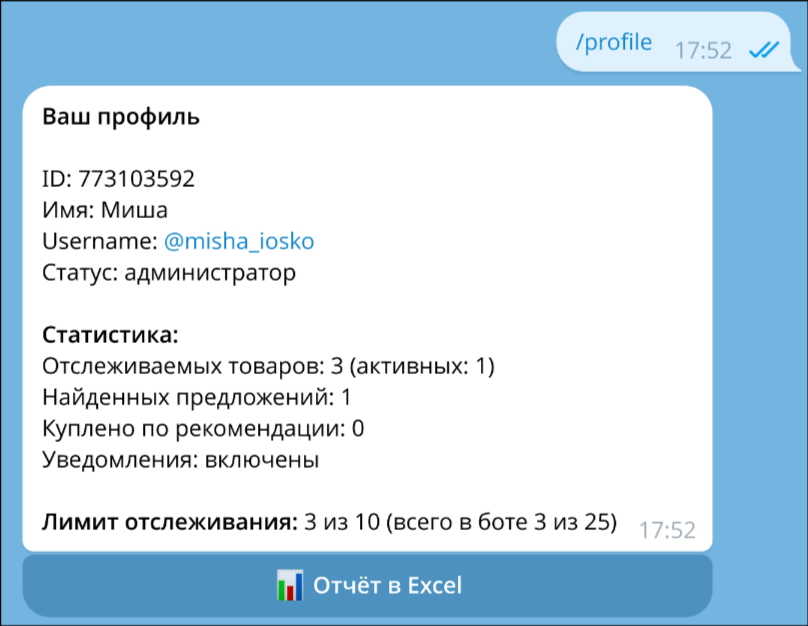
\includegraphics[scale=0.6]{kufar/screens/admin_profile.png}
	\caption{Профиль администратора}
	\label{fig:manual:admin_profile}
\end{figure}

\subsubsection{Отчёт о состоянии системы}

Под профилем расположена кнопка «Отчёт в \textit{Excel}». В меню отчётов администратор, помимо кнопок периода, видит кнопку «Состояние системы (30 дн.)». По ней бот присылает книгу \textit{Excel}, в которой собраны показатели за последние 30 дней:
\begin{itemize}
	\item число пользователей всего и активных;
	\item число отслеживаемых товаров и из них активных;
	\item число совпадений, найденных за период, и доставленных уведомлений;
	\item число совпадений, ожидающих доставки, и не доставленных после всех попыток;
	\item распределение отслеживаемых товаров по категориям.
\end{itemize}

По этому отчёту администратор видит, справляется ли система с нагрузкой. Растущее число ожидающих доставки совпадений означает, что уведомления не успевают уходить, а ненулевое число недоставленных говорит о том, что часть пользователей не получает сообщения. Пример отчёта приведён на рисунке~\ref{fig:manual:system_report}.

\begin{figure}[H]
	\centering
	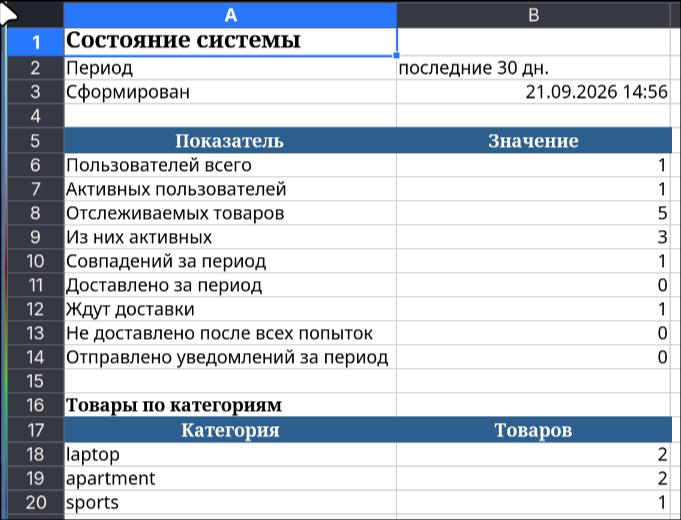
\includegraphics[scale=0.6]{kufar/screens/system_report.png}
	\caption{Отчёт о состоянии системы}
	\label{fig:manual:system_report}
\end{figure}

\subsubsection{Служебные оповещения}

Администратор получает от бота сообщения о событиях, которые требуют внимания человека:
\begin{itemize}
	\item площадка ответила отказом (код 403 или 429)~-- в сообщении указано, на сколько циклов приостановлена проверка, и что делать, если отказ повторяется: снизить общий лимит товаров или увеличить интервал опроса;
	\item контейнер системы запущен, остановлен штатно или упал с ненулевым кодом выхода;
	\item контейнер перестал проходить проверку работоспособности.
\end{itemize}

Одно и то же оповещение не повторяется подряд. Сообщение о блокировке площадкой приходит не чаще раза в 30 минут, о событиях контейнера не чаще раза в 5 минут. Если контейнер перезапускается чаще, в оповещении отдельно указано, что это похоже на цикл перезапусков. Пример оповещения показан на рисунке~\ref{fig:manual:admin_alert}.

\begin{figure}[H]
	\centering
	
\includegraphics[scale=0.6]{kufar/screens/admin_alert.png}
	\caption{Служебное оповещение администратору}
	\label{fig:manual:admin_alert}
\end{figure}

\subsubsection{Обслуживание сервера}

Часть задач администратор выполняет не в \textit{Telegram}, а на сервере. Все сервисы запускаются и обновляются одной командой \textit{Docker Compose}, журналы работы доступны там же. Резервные копии базы данных создаются автоматически раз в сутки в отдельном каталоге сервера. Пригодность последней копии проверяется сценарием восстановления, который загружает её во временную базу и выводит число строк в основных таблицах. Письма системы при стандартной настройке попадают в почтовый сервер-ловушку, который доступен в браузере на сервере; для доставки настоящим адресатам в файле окружения указываются параметры внешнего почтового сервера.

\subsection{Роль пользователя}
\label{sec:manual:user}

\subsubsection{Добавление отслеживаемого товара}

Добавление начинается с кнопки «Добавить товар» или команды /\textit{add}. Бот предлагает выбрать категорию из 13 вариантов. Первыми в списке стоят «Велосипед», «Ноутбук» и «Квартира (аренда)»: в них отбор ведётся по фильтрам самого \textit{Kufar.by} и получается заметно точнее. Над списком категорий находится кнопка «Вставить ссылку с \textit{Kufar}»; работа с ней описана далее. Экран выбора категории показан на рисунке~\ref{fig:manual:category}.

\begin{figure}[H]
	\centering
	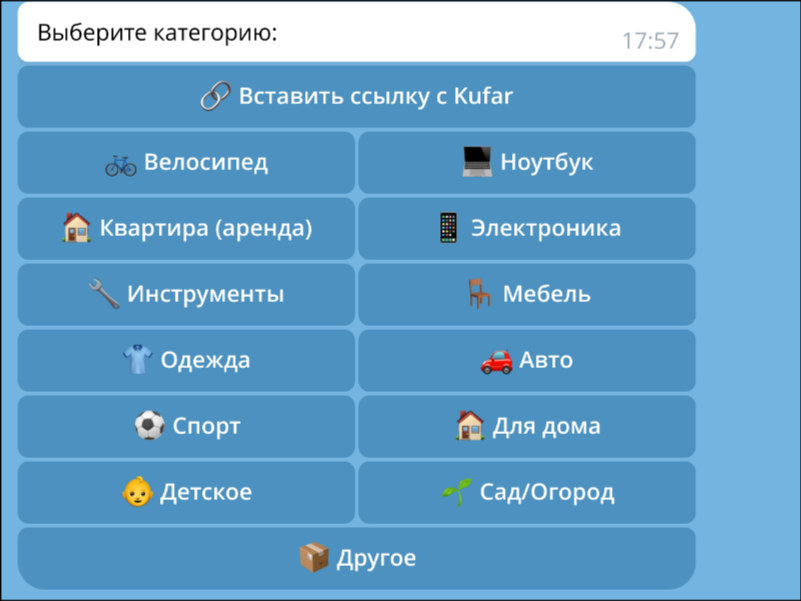
\includegraphics[scale=0.6]{kufar/screens/category.png}
	\caption{Выбор категории товара}
	\label{fig:manual:category}
\end{figure}

На следующем шаге вводится название товара: бренд и модель, например «\textit{Trek Marlin}» или «\textit{Pixel} 7\textit{a}». Лишних слов писать не стоит: бот требует, чтобы в объявлении встретилось каждое слово названия. В категориях с фильтрами площадки название можно пропустить кнопкой «Пропустить», тогда отбор выполнят фильтры.

Для велосипедов, ноутбуков и квартир бот открывает меню фильтров. В нём перечислены характеристики категории: для велосипеда это производитель, класс, размер рамы, диаметр колёс, материал рамы, для кого, состояние, регион и город. Пользователь открывает характеристику и отмечает одно или несколько значений; объявление подойдёт, если в нём есть любое из отмеченных. Длинные списки, например бренды или процессоры, разбиты на страницы по восемь значений. Кнопка «Сбросить» снимает выбор, «Назад» возвращает к списку характеристик, «Готово» завершает настройку. Сначала лучше выбрать регион: после этого список городов и районов сократится до выбранного региона. Меню фильтров показано на рисунке~\ref{fig:manual:filters}.

\begin{figure}[H]
	\centering
	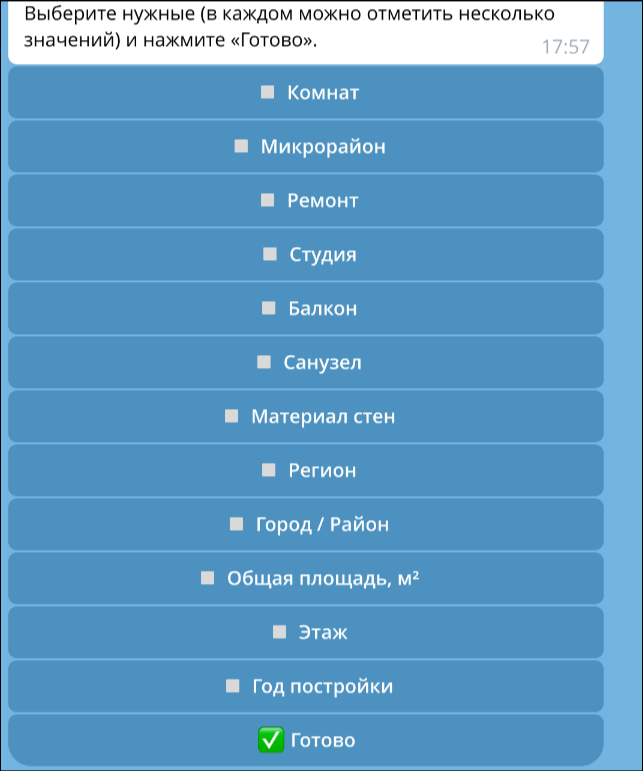
\includegraphics[scale=0.6]{kufar/screens/filters.png}
	\caption{Выбор значений фильтра}
	\label{fig:manual:filters}
\end{figure}

У квартир есть числовые фильтры: общая площадь, этаж и год постройки. Их значения вводятся сообщением в виде диапазона («45-70»), нижней границы («от 2015») или одного числа. Символ «-» сбрасывает фильтр.

Затем бот просит указать цену в белорусских рублях. Это минимальная цена, по которой товар сейчас продаётся на рынке: бот будет присылать объявления дешевле неё. На следующем шаге бот показывает стоп-слова, по которым объявления отсеиваются автоматически (например, «чехол» для электроники), и предлагает добавить свои слова-исключения через запятую, например «на запчасти, разбит». Шаг можно пропустить.

В конце бот показывает сводку: название, категорию, фильтры, цену и исключения. После подтверждения товар сохраняется, и бот сразу ищет на площадке объявления дешевле указанной цены. До пяти самых дешёвых из них приходят отдельным сообщением. Если таких объявлений нет, бот сообщает об этом и продолжает следить за площадкой. Результат мгновенного поиска показан на рисунке~\ref{fig:manual:instant}.

\begin{figure}[H]
	\centering
	
\includegraphics[scale=0.6]{kufar/screens/instant.png}
	\caption{Сохранение товара и мгновенный поиск}
	\label{fig:manual:instant}
\end{figure}

Добавить товар не получится, если занят личный лимит (3 товара) или общий лимит системы (25 товаров). Бот объясняет, какой из них достигнут. В первом случае нужно удалить ненужный товар в разделе «Мои товары», во втором остаётся подождать, пока место освободится.

На любом шаге диалог можно прервать кнопкой «Отмена», введённые данные при этом не сохраняются.

\subsubsection{Импорт фильтров из ссылки}

Если поиск уже настроен на сайте \textit{Kufar.by}, его не нужно повторять в боте. Пользователь настраивает фильтры на сайте или открывает свой сохранённый поиск, копирует ссылку из адресной строки и отправляет её боту после нажатия «Вставить ссылку с \textit{Kufar}». Бот переносит категорию, фильтры и цену и перечисляет неподдерживаемые параметры, например фильтр по станции метро. Цену из ссылки можно оставить одной кнопкой или ввести другую. Ссылку на страницу сохранённого поиска в личном кабинете бот принять не может, потому что её содержимое видно только владельцу, и подсказывает, какую ссылку прислать вместо неё.

\subsubsection{Получение уведомлений}

Когда на площадке появляется подходящее объявление, бот присылает сообщение. В заголовке указан тип события: «Новое предложение» или «Цена упала». В сообщении приведены цена (при снижении~-- старая зачёркнутая и новая), на сколько процентов цена ниже порога пользователя, состояние товара, местоположение, время публикации и ссылка «Открыть объявление». Первая фотография объявления идёт вместе с текстом, ещё до четырёх приходят следом альбомом. Пример уведомления показан на рисунке~\ref{fig:manual:notification}.

\begin{figure}[H]
	\centering
	
\includegraphics[scale=0.6]{kufar/screens/notification.png}
	\caption{Уведомление о выгодном предложении}
	\label{fig:manual:notification}
\end{figure}

Под уведомлением расположены кнопки «Интересно», «Не то» и «Куплю». Оценка сохраняется и попадает в отчёт, а число покупок по рекомендации бота видно в профиле. Одно и то же объявление повторно приходит только в том случае, если его цена стала ниже, чем в прошлом уведомлении. Чтобы уведомлений не было слишком много, по одному товару приходит не более 5 сообщений в час и не более 30 в сутки на пользователя; при большом числе находок первыми приходят самые дешёвые.

\subsubsection{Управление списком товаров}

Кнопка «Мои товары» или команда /\textit{my} открывает список отслеживаемых товаров. Над списком указано, сколько товаров отслеживается из личного лимита и сколько занято во всей системе. Под списком находятся кнопки «Экспорт \textit{CSV}» и «Импорт \textit{CSV}». Нажатие на товар открывает его карточку с категорией, ценой, фильтрами, статусом, словами-исключениями и автоматическими стоп-словами. Карточка товара показана на рисунке~\ref{fig:manual:product}.

\begin{figure}[H]
	\centering
	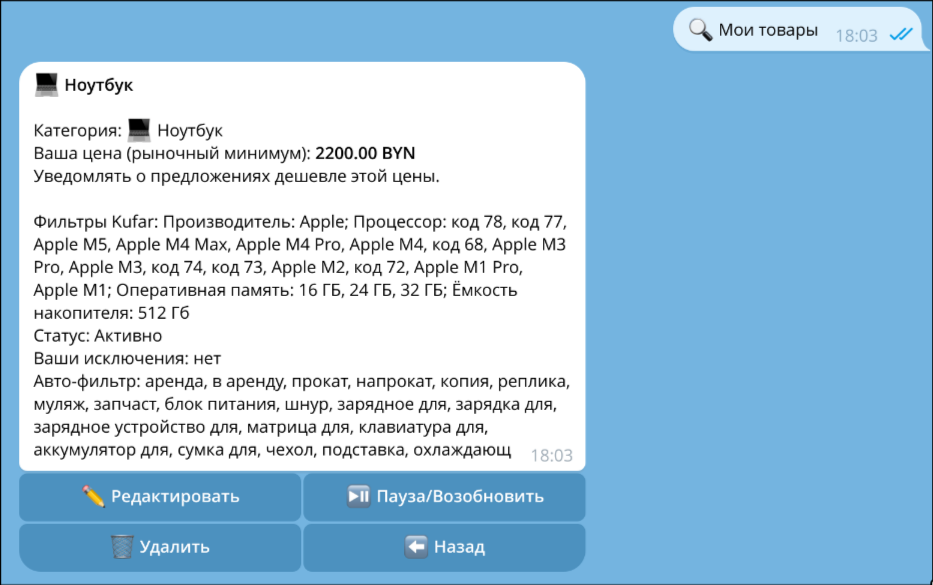
\includegraphics[scale=0.6]{kufar/screens/product.png}
	\caption{Карточка отслеживаемого товара}
	\label{fig:manual:product}
\end{figure}

В карточке доступны действия:
\begin{itemize}
	\item «Редактировать»~-- изменить название, цену, слова-исключения, а в категориях с фильтрами площадки и сами фильтры;
	\item «Пауза/Возобновить»~-- временно остановить отслеживание без удаления товара;
	\item «Удалить»~-- прекратить отслеживание и удалить товар;
	\item «Назад»~-- вернуться к списку.
\end{itemize}

Кнопка «Экспорт \textit{CSV}» присылает файл со списком товаров, который сразу открывается в \textit{Excel} по столбцам. Файл можно отредактировать и загрузить обратно кнопкой «Импорт \textit{CSV}», например чтобы перенести список на другую учётную запись. При импорте бот проверяет каждую строку так же, как при ручном вводе, и сообщает, сколько товаров добавлено, какие строки пропущены и почему.

\subsubsection{Настройки и электронная почта}

Кнопка «Настройки» или команда /\textit{settings} показывает, включены ли уведомления, выбранный язык и состояние электронной почты. Здесь можно отключить и снова включить уведомления, сменить язык интерфейса и перейти в раздел «Почта».

В разделе «Почта» пользователь нажимает «Привязать адрес» и вводит адрес электронной почты. На него приходит шестизначный код, который действует 15 минут; его нужно ввести в бота. Если письмо не пришло, код можно запросить снова, но не чаще раза в минуту. После подтверждения копии уведомлений раз в 5 минут приходят на почту сводным письмом, а отчёты можно получать вложением. Копии отключаются кнопкой в том же разделе, там же адрес можно сменить или отвязать.

\subsubsection{Профиль и отчёты}

Команда /\textit{profile} показывает идентификатор, имя, статус, число отслеживаемых и активных товаров, найденных предложений, покупок по рекомендации и занятость лимита. Кнопка «Отчёт в \textit{Excel}» под профилем или команда /\textit{report} предлагает выбрать период: 7, 30 или 90 дней. При подтверждённой почте появляются такие же кнопки для отправки отчёта письмом.

Отчёт состоит из двух листов. На листе «Находки» по одной строке на каждое найденное предложение: дата, товар, объявление, цена, порог, выгода в процентах, тип события, статус доставки, оценка и ссылка. Цены записаны числами, поэтому таблицу можно сортировать и фильтровать средствами \textit{Excel}. На листе «Итоги» указаны период, число находок и доставленных уведомлений, средняя выгода и лучшая находка. Пример отчёта приведён на рисунке~\ref{fig:manual:report}.

\begin{figure}[H]
	\centering
	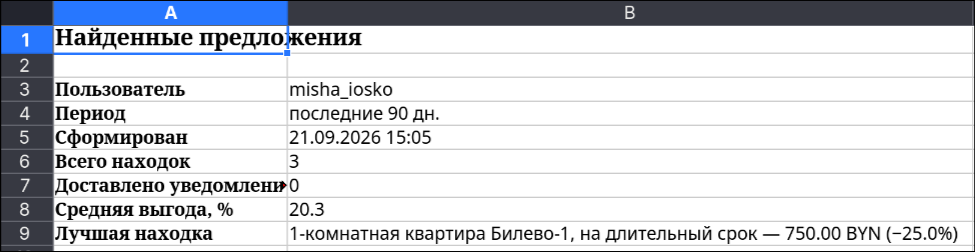
\includegraphics[scale=0.6]{kufar/screens/report.png}
	\caption{Отчёт о найденных предложениях}
	\label{fig:manual:report}
\end{figure}

\subsubsection{Действия при ошибках}

Бот отвечает на каждое действие. Если сервис временно недоступен, пользователь получает сообщение с просьбой повторить попытку через минуту. Если бот не понял сообщение, например диалог добавления прервался после перезапуска, пользователю предлагается начать заново кнопкой «Добавить». Команда /\textit{help} в любой момент показывает список команд и краткое описание работы бота.


	\sectioncentered*{Заключение}
\addcontentsline{toc}{section}{Заключение}

Цель курсового проекта достигнута: спроектирована и реализована автоматизированная информационная система отслеживания цен на товары в виде \textit{Telegram}-бота. Система каждые 3 минуты опрашивает площадку \textit{Kufar.by}, отбирает объявления дешевле заданной пользователем цены и уведомляет о новых предложениях и о снижении цены без повторов.

Анализ предметной области показывает, что ручной мониторинг не успевает за круглосуточным появлением объявлений, а существующие средства решают лишь часть задачи: сохранённые поиски площадки не отслеживают цену во времени, зарубежные трекеры рассчитаны на новые товары с артикулом, открытые боты ограничиваются текстовым поиском.

Ядро работы~-- база данных под управлением \textit{PostgreSQL}. \textit{ER}-модель в нотации Питера Чена из семи сущностей переходит в логическую и физическую схемы. Схема отвечает третьей нормальной форме, а отступления сделаны осознанно: \textit{JSON}-поля хранят фильтры категорий, журнал уведомлений~-- цену на момент отправки для проверки повторов. Индексы подобраны под запросы цикла опроса и доставки, прежде всего под поиск объявления по внешнему идентификатору~-- более 500 тысяч раз в сутки. Целостность поддерживают внешние ключи, ограничения уникальности и перечислимые типы.

Программная часть разделена на серверный сервис на \textit{FastAPI}, который выполняет SQL-запросы и периодические задачи, и бота на \textit{aiogram} для диалога с пользователем. Отбор по бренду, размеру рамы или числу комнат выполняет сама площадка. Система реализует весь функционал из постановки задачи: импорт фильтров из ссылки, мгновенный поиск, обмен списком товаров через \textit{CSV}, отчёты в \textit{Excel}, два языка интерфейса и копии уведомлений на почту.

Надёжность опирается на свойства СУБД. Найденное совпадение сначала фиксируется в базе данных, а отправляет его отдельная задача с повтором до пяти попыток; отметка о доставке и запись в журнал сохраняются одной транзакцией. Работу системы подтверждают более 280 автоматических тестов.

Система допускает развитие: модель данных предусматривает несколько площадок, поэтому к \textit{Kufar.by} добавляются \textit{Onliner}, \textit{av.by} и другие площадки. Система решает реальную задачу покупателей и перекупщиков: внешне это бот с кнопками, по существу~-- система обработки потока данных, качество которой определяет проектирование базы данных.


	% Зачем: Изменение надписи для списка литературы
% Почему: Пункт 2.8.1 Требований по оформлению пояснительной записки.
\renewcommand{\bibsection}{\sectioncentered*{Список использованных источников}}
\phantomsection\pagebreak % исправляет нумерацию в документе и исправляет гиперссылки в pdf
\addcontentsline{toc}{section}{Список использованных источников}

\sectioncentered*{Список использованных источников}

[1] \textit{Kufar.by}~-- площадка объявлений [Электронный ресурс].~-- Режим доступа: \textit{https://www.\allowbreak kufar.\allowbreak by}.~-- Дата доступа: 19.09.2026.

[2] \textit{CamelCamelCamel}~-- \textit{Amazon price tracker} [Электронный ресурс].~-- Режим доступа: \textit{https://camelcamelcamel.\allowbreak com}.~-- Дата доступа: 19.09.2026.

[3] \textit{Keepa}~-- \textit{Amazon price tracker} [Электронный ресурс].~-- Режим доступа: \textit{https://keepa.\allowbreak com}.~-- Дата доступа: 19.09.2026.

[4] \textit{Chen, P. P.} \textit{The Entity-Relationship Model~-- Toward a Unified View of Data} / \textit{P. P. Chen} // \textit{ACM Transactions on Database Systems}.~-- 1976.~-- \textit{Vol}.~1, \textit{No}.~1.~-- \textit{P}.~9--36.

[5] \textit{Brown, S. The C4 model for visualising software architecture} [Электронный ресурс].~-- Режим доступа: \textit{https://c4model.\allowbreak com}.~-- Дата доступа: 19.09.2026.

[6] \textit{Telegram Bot API} [Электронный ресурс].~-- Режим доступа: \textit{https://core.\allowbreak telegram.\allowbreak org/\allowbreak bots/\allowbreak api}.~-- Дата доступа: 19.09.2026.

[7] Документация к \textit{PostgreSQL}~16 [Электронный ресурс].~-- Режим доступа: \textit{https://postgrespro.\allowbreak ru/\allowbreak docs/\allowbreak postgresql/\allowbreak 16}.~-- Дата доступа: 19.09.2026.

[8] \textit{asyncpg Documentation} [Электронный ресурс].~-- Режим доступа: \textit{https://magicstack.\allowbreak github.\allowbreak io/\allowbreak asyncpg/}.~-- Дата доступа: 19.09.2026.

[9] \textit{Alembic Documentation} [Электронный ресурс].~-- Режим доступа: \textit{https://pypi.\allowbreak org/\allowbreak project/\allowbreak alembic}.~-- Дата доступа: 19.09.2026.

[10] \textit{FastAPI Documentation} [Электронный ресурс].~-- Режим доступа: \textit{https://fastapi.\allowbreak tiangolo.\allowbreak com}.~-- Дата доступа: 19.09.2026.

[11] \textit{aiogram~3 Documentation} [Электронный ресурс].~-- Режим доступа: \textit{https://docs.\allowbreak aiogram.\allowbreak dev}.~-- Дата доступа: 19.09.2026.

[12] \textit{APScheduler Documentation} [Электронный ресурс].~-- Режим доступа: \textit{https://apscheduler.\allowbreak readthedocs.\allowbreak io}.~-- Дата доступа: 19.09.2026.

[13] \textit{Docker Compose Documentation} [Электронный ресурс].~-- Режим доступа: \textit{https://docs.\allowbreak docker.\allowbreak com/\allowbreak compose/}.~-- Дата доступа: 19.09.2026.

[14] СТП 01-2024. Стандарт предприятия. Дипломные проекты (работы). Общие требования.~-- Минск: БГУИР, 2024.~-- 169 с.


	\clearpage
\phantomsection
\begin{center}
	\textbf{ПРИЛОЖЕНИЕ А}\\
	(обязательное)\\
	\textbf{Листинг основных функций программного модуля}
\end{center}
\appendixtocline{Приложение А (обязательное) Листинг основных функций программного модуля}

\lstset{
  language=SQL,
  showstringspaces=false,
  breaklines=true,
  breakatwhitespace=true,
  tabsize=4,
  columns=fullflexible,
  keepspaces=true,
}

\lstinputlisting{attachments/kufar/schema.sql}


	\renewcommand{\bibsection}{\sectioncentered*{Ведомость курсового проекта}}
\phantomsection\pagebreak % исправляет нумерацию в документе и исправляет гиперссылки в pdf

\IfFileExists{vedomost.pdf}{
\includepdf[pages = 1]{vedomost.pdf}
}{
  \centering \textit{Файл vedomost.pdf не найден. Пожалуйста, добавьте его для включения ведомости в документ.}
}
\end{document}
